\documentclass[12pt]{amsart}
\usepackage[utf8]{inputenc}
% Packages
\RequirePackage{amsmath,amssymb,amsthm}
\RequirePackage{amsfonts}
%\RequirePackage{geometry}
\RequirePackage{color}
\RequirePackage{mathtools}
\RequirePackage{bbm}
\RequirePackage{amsfonts}
\RequirePackage{mathrsfs}
\RequirePackage{tikz}
\usepackage[shortlabels]{enumitem}
\usetikzlibrary{shapes.geometric, arrows}
\usetikzlibrary{decorations.pathmorphing}
\usetikzlibrary{cd}
\tikzstyle{arrow} = [thick,->,>=stealth]

% Arrows
\providecommand{\po}{\arrow[ul,phantom,"\ulcorner" very near start]}
\providecommand{\pb}{\arrow[dr,phantom,"\lrcorner" very near start]}
\providecommand{\xto}[1]{\xrightarrow{#1}}
\providecommand{\from}{\leftarrow}
\providecommand{\xfrom}[1]{\overset{#1}{\leftarrow}}

\providecommand{\mapsfrom}{\mathrel{\reflectbox{\ensuremath{\mapsto}}}}
\providecommand{\longmapsfrom}{\mathrel{\reflectbox{\ensuremath{\longmapsto}}}}

\providecommand{\hookto}{\xhookrightarrow{}}
\providecommand{\xhookto}[1]{\overset{#1}{\hookrightarrow}}

\providecommand{\hookfrom}{\xhookleftarrow{}}
\providecommand{\xhookfrom}[1]{\xhookleftarrow{#1}}

\providecommand{\tto}{\twoheadrightarrow}
\providecommand{\xtto}[1]{\overset{#1}{\twoheadrightarrow}}
\providecommand{\ffrom}{\twoheadleftarrow}
\providecommand{\xffrom}[1]{\overset{#1}{\ffrom}}

\providecommand{\ladjoint}[2]{ #1\rightleftarrows #2 }
\makeatletter
\providecommand{\superimpose}[2]{%
  {\ooalign{$#1\@firstoftwo#2$\cr\hfil$#1\@secondoftwo#2$\hfil\cr}}}
\makeatother
\providecommand{\smallslash}{\mbox{\tiny/}}

\providecommand{\clhookto}{\mathrel{\raisebox{0.1em}{$\mathrel{\mathpalette\superimpose{{\hspace{0.1cm}\vspace{0.1em}\smallslash}{\hookrightarrow}}}$}}}
\providecommand{\xclhook}[1]{\overset{#1}{\clhook}}

\providecommand{\clhookfrom}{\mathrel{\raisebox{0.1em}{$\mathrel{\mathpalette\superimpose{{\hspace{0.1cm}\vspace{0.1em}\smallslash}{\hookleftarrow}}}$}}}

\providecommand{\ohookto}{\mathrel{\raisebox{0.03em}{$\mathrel{\mathpalette\superimpose{{\hspace{0.1cm}\vspace{0.03em}\mbox{\small$\circ$}}{\hookrightarrow}}}$}}}

\providecommand{\ohookfrom}{\mathrel{\raisebox{0.03em}{$\mathrel{\mathpalette\superimpose{{\hspace{0.1cm}\vspace{0.03em}\mbox{\small$\circ$}}{\hookleftarrow}}}$}}}

\providecommand{\cofto}{\rightarrowtail}
\providecommand{\coffrom}{\leftarrowtail}
\providecommand{\xcofto}[1]{\overset{#1}{\cofto}}
\providecommand{\xcoffrom}[1]{\overset{#1}{\coffrom}}

% Common Text Commands
\providecommand{\ab}{\text{ab}}
\providecommand{\ann}{\text{ann}}
\providecommand{\Aut}{\text{Aut}}
\providecommand{\char}{\text{char}}
\providecommand{\cl}{\text{cl}}
\providecommand{\codim}{\text{codim}}
\providecommand{\coev}{\text{coev}}
\providecommand{\colim}{\text{colim}}
\providecommand{\conj}{\text{conj}}
\providecommand{\const}{\text{const}}
\providecommand{\Disc}{\text{Disc}}
\providecommand{\End}{\text{End}}
\providecommand{\EKL}{\text{EKL}}
\providecommand{\ev}{\text{ev}}
\providecommand{\Fix}{\text{Fix}}
\providecommand{\Frac}{\text{Frac}}
\providecommand{\Frob}{\text{Frob}}
\providecommand{\Fun}{\text{Fun}}
\providecommand{\Gal}{\text{Gal}}
\providecommand{\GL}{\text{GL}}
\providecommand{\gr}{\text{gr}}
\newcommand{\GW}{\text{GW}}
\providecommand{\Hom}{\text{Hom}}
\providecommand{\id}{\text{id}}
\providecommand{\im}{\text{im}}
\renewcommand{\Im}{\text{Im}}
\providecommand{\incl}{\text{incl}}
\providecommand{\Ind}{\text{Ind}}
\providecommand{\Inn}{\text{Inn}}
\providecommand{\Jac}{\text{Jac}}
\providecommand{\Map}{\text{Map}}
\providecommand{\mult}{\text{mult}}
\providecommand{\op}{\text{op}}
\providecommand{\Orb}{\text{Orb}}
\providecommand{\ord}{\text{ord}}
\providecommand{\Out}{\text{Out}}
\providecommand{\Perm}{\text{Perm}}
\providecommand{\pr}{\text{pr}}
\providecommand{\pre}{\text{pre}}
\providecommand{\PSL}{\text{PSL}}
\providecommand{\quot}{\text{quot}}
\providecommand{\rank}{\text{rank}}
\renewcommand{\Re}{\text{Re}}
\providecommand{\Res}{\text{Res}}
\providecommand{\sgn}{\text{sgn}}
\providecommand{\sig}{\text{sig}}
\providecommand{\SL}{\text{SL}}
\providecommand{\soc}{\text{soc}}
\providecommand{\spn}{\text{span}}
\providecommand{\Spec}{\text{Spec}\hspace{0.1em}}
\providecommand{\Stab}{\text{Stab}}
\providecommand{\supp}{\text{supp}}
\providecommand{\Syl}{\text{Syl}}
\providecommand{\syl}{\text{syl}}
\providecommand{\Sym}{\text{Sym}}
\providecommand{\Tor}{\text{Tor}}
\providecommand{\Tr}{\text{Tr}}

% BB Sets
\providecommand{\A}{\mathbb{A}}
\providecommand{\C}{\mathbb{C}}
\providecommand{\F}{\mathbb{F}}
\providecommand{\N}{\mathbb{N}}
\providecommand{\P}{\mathbb{P}}
\providecommand{\Q}{\mathbb{Q}}
\providecommand{\R}{\mathbb{R}}
\providecommand{\Z}{\mathbb{Z}}

% Commands
\providecommand{\lrangle}[1]{\left\langle #1 \right\rangle}
\providecommand{\nsubgp}{\trianglelefteq}
\providecommand{\p}{\mathfrak{p}}
\renewcommand{\H}{\textbf{H}}
\newcommand{\gw}[1]{\left\langle #1 \right\rangle}
\newcommand{\ovl}[1]{\overline{#1}}

\let\minus\smallsetminus
\let\bar\overline
\let\smsh\wedge

\providecommand{\SH}{\mathcal{SH}}


% Colors
\providecommand{\green}[1]{\textcolor{green}{#1}}
\providecommand{\red}[1]{\textcolor{red}{#1}}
\providecommand{\orange}[1]{\textcolor{orange}{#1}}
\providecommand{\green}[1]{\textcolor{green}{#1}}
\providecommand{\blue}[1]{\textcolor{blue}{#1}}
\providecommand{\purple}[1]{\textcolor{purple}{#1}}

\RequirePackage{amsmath,amssymb}
\RequirePackage{geometry}

% AT commands
\providecommand{\BG}{\text{BG}}
\providecommand{\BO}{\text{BO}}
\providecommand{\BP}{\text{BP}}
\providecommand{\BU}{\text{BU}}
\providecommand{\BSO}{\text{BSO}}
\providecommand{\BSU}{\text{BSU}}
\providecommand{\BGL}{\text{BGL}}
\providecommand{\coeq}{\text{coeq}}
\providecommand{\cof}{\text{cof}}
\providecommand{\cone}{\text{cone}}
\providecommand{\eq}{\text{eq}}
\providecommand{\EU}{\text{EU}}
\providecommand{\Ex}{\text{Ex}}
\providecommand{\Ext}{\text{Ext}}
\providecommand{\Gr}{\text{Gr}}
\providecommand{\Ho}{\text{Ho}}
\providecommand{\hocofib}{\text{hocofib}}
\providecommand{\hocolim}{\text{hocolim}}
\providecommand{\holim}{\text{holim}}
\providecommand{\KGL}{\text{KGL}}
\providecommand{\ko}{\text{ko}}
\providecommand{\KO}{\text{KO}}
\providecommand{\kq}{\text{kq}}
\providecommand{\KQ}{\text{KQ}}
\providecommand{\KR}{\text{KR}}
\providecommand{\ku}{\text{ku}}
\providecommand{\KU}{\text{KU}}
\providecommand{\Lan}{\text{Lan}}
\providecommand{\MGL}{\text{MGL}}
\providecommand{\MO}{\text{MO}}
\providecommand{\MSL}{\text{MSL}}
\providecommand{\MSO}{\text{MSO}}
\providecommand{\MSp}{\text{MSp}}
\providecommand{\MU}{\text{MU}}
\providecommand{\Out}{\text{Out}}
\providecommand{\pre}{\text{pre}}
\providecommand{\Ran}{\text{Ran}}
\providecommand{\RO}{\text{RO}}
\providecommand{\Sing}{\text{Sing}}
\providecommand{\SO}{\text{SO}}
\providecommand{\Spin}{\text{Spin}}
\providecommand{\Sq}{\text{Sq}}
\providecommand{\SU}{\text{SU}}
\providecommand{\Sym}{\text{Sym}}
\providecommand{\TC}{\text{TC}}
\providecommand{\Th}{\text{Th}}
\providecommand{\THH}{\text{THH}}
\providecommand{\TP}{\text{TP}}
\providecommand{\TR}{\text{TR}}
\providecommand{\SH}{\mathcal{SH}}
\providecommand{\Sp}{\textit{Sp}}

% Chromatic
\providecommand{\Prin}{\text{Prin}}
\providecommand{\FGL}{\texttt{FGL}}
\providecommand{\SI}{\texttt{SI}}
\providecommand{\FG}{\text{FG}}
\providecommand{\fg}{\text{fg}}




% Spaces
\providecommand{\CP}{\mathbb{C}\text{P}}
\providecommand{\HP}{\mathbb{H}\text{P}}
\providecommand{\RP}{\mathbb{R}\text{P}}

% Other
\providecommand{\Cech}{\check{C}}
\let\adj\dashv
\let\smashprod\wedge


% Custom Arrows
% 
% (c) Thomas Brazelton
%
%% This program can be redistributed and/or modified under the terms
%% of the LaTeX Project Public License Distributed from CTAN archives
%% in directory macros/latex/base/lppl.txt.
% 

% Packages
\RequirePackage{amsmath,amssymb}
\RequirePackage{amsfonts}
\RequirePackage{geometry}
%\RequirePackage{hyperref}
\RequirePackage{color}
\RequirePackage{mathtools}		% used for arrows
%\RequirePackage{ bbold }
\RequirePackage{bbm}
\RequirePackage{amsfonts}
\RequirePackage{mathrsfs}
\RequirePackage{tikz}
%\usepackage[shortlabels]{enumitem}
\usetikzlibrary{shapes.geometric, arrows}
\usetikzlibrary{decorations.pathmorphing}
\usetikzlibrary{cd}
\tikzstyle{arrow} = [thick,->,>=stealth]


% Arrows
\providecommand{\po}{\arrow[ul,phantom,"\ulcorner" very near start]}
\providecommand{\pb}{\arrow[dr,phantom,"\lrcorner" very near start]}
\providecommand{\pol}{\arrow[ur,phantom,"\urcorner" very near start]}
\providecommand{\pbr}{\arrow[dl,phantom,"\llcorner" very near start]}
\providecommand{\xto}[1]{\xrightarrow{#1}}
\providecommand{\from}{\leftarrow}
\providecommand{\xfrom}[1]{\overset{#1}{\leftarrow}}

\providecommand{\mapsfrom}{\mathrel{\reflectbox{\ensuremath{\mapsto}}}}
\providecommand{\longmapsfrom}{\mathrel{\reflectbox{\ensuremath{\longmapsto}}}}

\providecommand{\hookto}{\xhookrightarrow{}}
\providecommand{\xhookto}[1]{\overset{#1}{\hookrightarrow}}

\providecommand{\hookfrom}{\xhookleftarrow{}}
\providecommand{\xhookfrom}[1]{\xhookleftarrow{#1}}

\providecommand{\tto}{\twoheadrightarrow}
\providecommand{\xtto}[1]{\overset{#1}{\twoheadrightarrow}}
\providecommand{\ffrom}{\twoheadleftarrow}
\providecommand{\xffrom}[1]{\overset{#1}{\ffrom}}

\providecommand{\ladjoint}[2]{ #1\rightleftarrows #2 }
\makeatletter
\providecommand{\superimpose}[2]{%
  {\ooalign{$#1\@firstoftwo#2$\cr\hfil$#1\@secondoftwo#2$\hfil\cr}}}
\makeatother
\providecommand{\smallslash}{\mbox{\tiny/}}

\providecommand{\clhookto}{\mathrel{\raisebox{0.1em}{$\mathrel{\mathpalette\superimpose{{\hspace{0.1cm}\vspace{0.1em}\smallslash}{\hookrightarrow}}}$}}}
\providecommand{\xclhook}[1]{\overset{#1}{\clhook}}

\providecommand{\clhookfrom}{\mathrel{\raisebox{0.1em}{$\mathrel{\mathpalette\superimpose{{\hspace{0.1cm}\vspace{0.1em}\smallslash}{\hookleftarrow}}}$}}}

\providecommand{\ohookto}{\mathrel{\raisebox{0.03em}{$\mathrel{\mathpalette\superimpose{{\hspace{0.1cm}\vspace{0.03em}\mbox{\small$\circ$}}{\hookrightarrow}}}$}}}

\providecommand{\ohookfrom}{\mathrel{\raisebox{0.03em}{$\mathrel{\mathpalette\superimpose{{\hspace{0.1cm}\vspace{0.03em}\mbox{\small$\circ$}}{\hookleftarrow}}}$}}}

\providecommand{\cofto}{\rightarrowtail}
\providecommand{\coffrom}{\leftarrowtail}
\providecommand{\xcofto}[1]{\overset{#1}{\cofto}}
\providecommand{\xcoffrom}[1]{\overset{#1}{\coffrom}}

\providecommand{\lllarrows}{\mathrel{\substack{\textstyle\leftarrow\\[-0.6ex] \textstyle\leftarrow \\[-0.6ex] \textstyle\leftarrow}}}



\providecommand{\rrrarrows}{\mathrel{\substack{\textstyle\rightarrow\\[-0.6ex] \textstyle\rightarrow \\[-0.6ex] \textstyle\rightarrow}}}

\providecommand{\rlrarrows}{\mathrel{\substack{\textstyle\rightarrow\\[-0.6ex] \textstyle\lefttarrow \\[-0.6ex] \textstyle\rightarrow}}}


\RequirePackage{cust-package-free}






% BB Sets
\providecommand{\C}{\mathbb{C}}
\providecommand{\F}{\mathbb{F}}
\providecommand{\N}{\mathbb{N}}
\providecommand{\Q}{\mathbb{Q}}
\providecommand{\R}{\mathbb{R}}
\providecommand{\Z}{\mathbb{Z}}

% Projective
\providecommand{\CP}{\mathbb{C}\text{P}}
\providecommand{\RP}{\mathbb{R}\text{P}}

% Colors
\providecommand{\green}[1]{\textcolor{green}{#1}}
\providecommand{\red}[1]{\textcolor{red}{#1}}
\providecommand{\orange}[1]{\textcolor{orange}{#1}}
\providecommand{\green}[1]{\textcolor{green}{#1}}
\providecommand{\blue}[1]{\textcolor{blue}{#1}}
\providecommand{\purple}[1]{\textcolor{purple}{#1}}

% Commands
\providecommand{\ceil}[1]{\left\lceil #1 \right\rceil}
\providecommand{\floor}[1]{\left\lfloor #1 \right\rfloor}
\providecommand{\lrangle}[1]{\left\langle #1 \right\rangle}
\providecommand{\und}[1]{\underline{#1}}
\renewcommand{\hat}{\widehat}
\providecommand{\legendre}[2]{\left( \substack{#1 \\ #2} \right)}
\providecommand{\trianglerightneq}{\mathrel{\ooalign{\raisebox{-0.5ex}{\reflectbox{\rotatebox{90}{$\nshortmid$}}}\cr$\triangleright$\cr}\mkern-3mu}}
\providecommand{\triangleleftneq}{\mathrel{\reflectbox{$\trianglerightneq$}}}

% Other
\providecommand{\dot}{\bullet}
\let\oldemptyset\emptyset
\let\emptyset\varnothing
\providecommand{\setminus}{\smallsetminus}
\providecommand{\minus}{\smallsetminus}
\let\bar\overline
\let\tilde\widetilde
\let\til\widetilde
\let\nsubgp\trianglelefteq
\let\del\partial
\let\epsilon\varepsilon
\providecommand{\bigast}{\mathop{\scalebox{1.5}{\raisebox{-0.2ex}{$\ast$}}}}
\providecommand{\llangle}{\left\langle\hspace{-0.2em}\left\langle}
\providecommand{\rrangle}{\right\rangle\hspace{-0.2em}\right\rangle}
\providecommand{\Pfister}[1]{\llangle #1 \rrangle}


% operp command for quadratic forms, from mathabx.sty
% https://tex.stackexchange.com/a/61882/
\DeclareFontFamily{U}{matha}{\hyphenchar\font45}
\DeclareFontShape{U}{matha}{m}{n}{
      <5> <6> <7> <8> <9> <10> gen * matha
      <10.95> matha10 <12> <14.4> <17.28> <20.74> <24.88> matha12
      }{}
\DeclareSymbolFont{matha}{U}{matha}{m}{n}
\DeclareFontFamily{U}{mathx}{\hyphenchar\font45}
\DeclareFontShape{U}{mathx}{m}{n}{
      <5> <6> <7> <8> <9> <10>
      <10.95> <12> <14.4> <17.28> <20.74> <24.88>
      mathx10
      }{}
\DeclareSymbolFont{mathx}{U}{mathx}{m}{n}
\DeclareMathSymbol{\operp}         {2}{matha}{"6B}
\DeclareMathSymbol{\bigoperp}       {1}{mathx}{"CB}



%%
%% End of file `custom-arrows.sty'.

\RequirePackage{amsmath,amssymb,amsfonts}
\RequirePackage{bbm}


% Categories
\providecommand{\onecat}{\mathbbm{1}}
\providecommand{\twocat}{\mathbbm{2}}
\providecommand{\Alg}{\texttt{Alg}}
\providecommand{\Ab}{\texttt{Ab}}
\providecommand{\CAlg}{\texttt{CAlg}}
\providecommand{\Cat}{\texttt{Cat}}
\providecommand{\CDGA}{\texttt{CDGA}}
\providecommand{\CG}{\texttt{CG}}
\providecommand{\CGWH}{\texttt{CGWH}}
\providecommand{\Ch}{\texttt{Ch}}
\providecommand{\CAlg}{\texttt{CAlg}}
\providecommand{\CMon}{\texttt{CMon}}
\providecommand{\coAlg}{\texttt{coAlg}}
\providecommand{\coMod}{\texttt{coMod}}
\providecommand{\Coh}{\texttt{Coh}}
\providecommand{\CommRing}{\texttt{CommRing}}
\providecommand{\Corr}{\texttt{Corr}}
\providecommand{\CRing}{\texttt{CRing}}
\providecommand{\CW}{\texttt{CW}}
\providecommand{\Field}{\texttt{Field}}
\providecommand{\Fin}{\texttt{Fin}}
\providecommand{\FinSet}{\texttt{FinSet}}
\providecommand{\Grp}{\texttt{Grp}}
\providecommand{\Grpd}{\texttt{Grpd}}
\providecommand{\Grph}{\texttt{Grph}}
\providecommand{\Kar}{\texttt{Kar}}
\providecommand{\Kan}{\texttt{Kan}}
\providecommand{\Mod}{\texttt{Mod}}
\providecommand{\lmod}[1]{#1\text{-}\texttt{Mod}}
\providecommand{\rmod}[1]{\texttt{Mod}\text{-}#1}
\providecommand{\bimod}[2]{#1\text{-}\texttt{Mod}\text{-}#2}
\providecommand{\Ouv}{\texttt{Ouv}}
\providecommand{\Poset}{\texttt{Poset}}
\providecommand{\PSh}{\texttt{PSh}}
\providecommand{\PShv}{\texttt{PShv}}
\providecommand{\qCat}{\texttt{qCat}}
\providecommand{\QCoh}{\texttt{QCoh}}
\providecommand{\Rep}{\texttt{Rep}}
\providecommand{\Ring}{\texttt{Ring}}
\providecommand{\Set}{\texttt{Set}}
\providecommand{\SH}{\mathcal{SH}}
\providecommand{\Sh}{\texttt{Sh}}
\providecommand{\Shv}{\texttt{Shv}}
\providecommand{\Spectra}{\texttt{Spectra}}
\providecommand{\sAb}{\text{sAb}}
\providecommand{\sSet}{\texttt{sSet}}
\providecommand{\Stack}{\texttt{Stack}}
\providecommand{\Top}{\texttt{Top}}
\providecommand{\Ring}{\texttt{Ring}}
\providecommand{\Vect}{\texttt{Vect}}

% Other
\providecommand{\cyc}{\text{cyc}}
\providecommand{\dg}{\text{dg}}
\providecommand{\gen}{\text{gen}}
\providecommand{\inj}{\text{inj}}
\providecommand{\mor}{\text{mor}}
\providecommand{\Mor}{\text{Mor}}
\providecommand{\ob}{\text{ob}}
\providecommand{\obj}{\text{obj}}
\providecommand{\proj}{\text{proj}}
\providecommand{\Span}{\text{Span}}

\newcommand{\DDelta}{\bm{\Delta}}


% Limits
\providecommand{\llim}{\varprojlim}
\providecommand{\rlim}{\varinjlim}




\usepackage{caption}
\usepackage{longtable}
\usepackage{quiver}
\usepackage{mdframed}
\usepackage{float}
\setlength{\parindent}{0em}
\setlength{\parskip}{0.5em}

\renewcommand{\P}{\mathbb{P}}
\let\til\widetilde



% Copied
\usepackage{xcolor}
\providecommand{\gray}[1]{\color{gray}#1 \color{black}}
\definecolor{purple}{RGB}{128, 0, 255} 
\renewcommand{\purple}[1]{\color{purple}#1 \color{black}}

\definecolor{darkgreen}{rgb}{0,0.30,0}
\renewcommand{\green}[1]{\color{darkgreen}#1 \color{black}}

\definecolor{darkred}{rgb}{0.75,0,0}
\newcommand{\darkred}[1]{\color{darkred}#1 \color{black}}

\definecolor{darkblue}{rgb}{0,0,0.6} 
\usepackage{amsthm,thmtools}
\usepackage[pdfborder=0,pagebackref,colorlinks,citecolor=darkgreen,linkcolor=darkgreen,urlcolor=darkblue]{hyperref}
\usepackage{cleveref}
    \let\fullref\autoref
%
%  \autoref is very crude.  It uses counters to distinguish environments
%  so that if say {lemma} uses the {theorem} counter, then autrorefs
%  which should come out Lemma X.Y in fact come out Theorem X.Y.  To
%  correct this give each its own counter eg:
%                 \newtheorem{theorem}{Theorem}[section]
%                 \newtheorem{lemma}{Lemma}[section]
%  and then equate the counters by commands like:
%                 \makeatletter
%                   \let\c@lemma\c@theorem
%                  \makeatother
%
%  To work correctly the environment name must have a corrresponding 
%  \XXXautorefname defined.  The following command does the job:
%
\def\makeautorefname#1#2{\expandafter\def\csname#1autorefname\endcsname{#2}}
%
%  Some standard autorefnames.  If the environment name for an autoref 
%  you need is not listed below, add a similar line to your TeX file:
%  
\makeautorefname{eqn}{Equation}%
\makeautorefname{sec}{Section}%
\makeautorefname{subsec}{Subsection}%
\makeautorefname{footnote}{footnote}%
\makeautorefname{item}{item}%
\makeautorefname{figure}{Figure}%
\makeautorefname{table}{Table}%
\makeautorefname{part}{Part}%
\makeautorefname{app}{Appendix}%
\makeautorefname{cla}{claim}%
\makeautorefname{conj}{conjecture}%
\makeautorefname{cor}{corollary}%
\makeautorefname{cex}{counterexample}%
\makeautorefname{cexs}{counterexamples}%
\makeautorefname{dig}{digression}%
\makeautorefname{disc}{discussion}%
\makeautorefname{def}{definition}%
\makeautorefname{ex}{example}%
\makeautorefname{exs}{examples}%
\makeautorefname{fac}{fact}%
\makeautorefname{intu}{intuition}%
\makeautorefname{lem}{lemma}%
\makeautorefname{meta}{metathm}%
\makeautorefname{nota}{notation}%
\makeautorefname{note}{note}%
\makeautorefname{prop}{proposition}%
\makeautorefname{rmk}{remark}%
\makeautorefname{term}{terminology}%
\makeautorefname{thm}{theorem}%
\makeautorefname{upsh}{upshot}%
%
%                  *** End of hyperref stuff ***



\theoremstyle{definition}
\newtheorem{theorem}{Theorem}[section]
\newtheorem{claim}[theorem]{Claim}
\newtheorem{conjecture}[theorem]{Conjecture}
\newtheorem{corollary}[theorem]{Corollary}
\newtheorem{counterexample}[theorem]{Counterexample}
\newtheorem{definition}[theorem]{Definition}
\newtheorem{digression}[theorem]{Digression}
\newtheorem{example}[theorem]{Example}
\newtheorem{examples}[theorem]{Examples}
\newtheorem{exercise}[theorem]{Exercise}
\newtheorem{fact}[theorem]{Fact}
\newtheorem{idea}[theorem]{Idea}
\newtheorem{intuition}[theorem]{Intuition}
\newtheorem{lemma}[theorem]{Lemma}
\newtheorem{metathm}[theorem]{Meta-theorem}

\newtheorem{notation}[theorem]{Notation}
\newtheorem{note}[theorem]{Note}
\newtheorem{proposition}[theorem]{Proposition}
\newtheorem{remark}[theorem]{Remark}
\newtheorem{terminology}[theorem]{Terminology}
\newtheorem{upshot}[theorem]{Upshot}



%\newtheorem{warning}[theorem]{Warning}

%%%% hack to get fullref working correctly
\makeatletter
\let\c@corollary=\c@theorem
\let\c@proposition=\c@theorem
\let\c@lemma=\c@theorem
\let\c@conjecture=\c@theorem
\let\c@definition=\c@theorem
\let\c@example=\c@theorem
\let\c@remark=\c@theorem
\let\c@notation=\c@theorem
\let\c@equation\c@theorem
\makeatother

\renewcommand*{\subsectionautorefname}{Subsection}
%%%%%%%%%%%%%%%%%%%%%%%%%%%%%%%%%%%%%%%%%%%%%%
\usepackage[color=lightblue,textsize=tiny]{todonotes}

\usepackage{fancyhdr}
\pagestyle{fancy}
\fancyhf{}
% \fancyhead[L]{\small\itshape\thespeaker}
% \fancyhead[R]{\small\itshape\theday, \theyear}
\fancyhead[C]{\small\itshape {\color{gray} Last compiled: \today}}
\fancyfoot[C]{\small {\thepage}}



\newcommand{\HZ}{H\widetilde{\mathbb{Z}}}

\providecommand{\GOS}{G\mathcal{O}\mathcal{S}}
\providecommand{\Pic}{\text{Pic}}
\providecommand{\Perf}{\text{Perf}}

\newcommand{\fiberq}[3]{\frac{#1}{#2}\hspace{-0.2em}{}_{#3}}

\renewcommand{\O}{\mathcal{O}}
\renewcommand{\Th}{\text{Th}}
\providecommand{\KO}{\text{KO}}

\let\del\partial
\providecommand{\soc}{\text{soc}}
\providecommand{\Sm}{\text{Sm}}
\providecommand{\ind}{\text{ind}}
\providecommand{\Vect}{\textit{Vect}}
\providecommand{\Char}{\text{char}}
\let\smashprod\wedge
\providecommand{\Sp}{\texttt{Sp}}
\providecommand{\TM}{\text{TM}}

\providecommand{\pt}{\text{pt}}

\providecommand{\Cof}{\text{Cof}}
\providecommand{\Fib}{\text{Fib}}
\providecommand{\LLP}{\text{LLP}}
\providecommand{\RLP}{\text{RLP}}
\let\emptyset\varnothing
\providecommand{\Cyl}{\text{Cyl}}

\providecommand{\Cell}{\text{Cell}}
\providecommand{\SP}{\text{SP}}
\providecommand{\Assoc}{\text{Assoc}}
\providecommand{\Comm}{\text{Comm}}
\providecommand{\hQCat}{\texttt{hQCat}}
\providecommand{\St}{\text{St}}
\providecommand{\Unst}{\text{Unst}}
\providecommand{\coCart}{\text{coCart}}
\providecommand{\Tw}{\text{Tw}}
\providecommand{\Ev}{\text{Ev}}
\providecommand{\LFib}{\text{LFib}}
\providecommand{\lax}{\text{lax}}

\providecommand{\Sp}{\text{Sp}}
\providecommand{\PSp}{\text{PSp}}

\title{Higher Algebra}

\author{Maximilien P\'eroux}
\date{\today}




\begin{document}

\maketitle

\begin{figure}[h]
  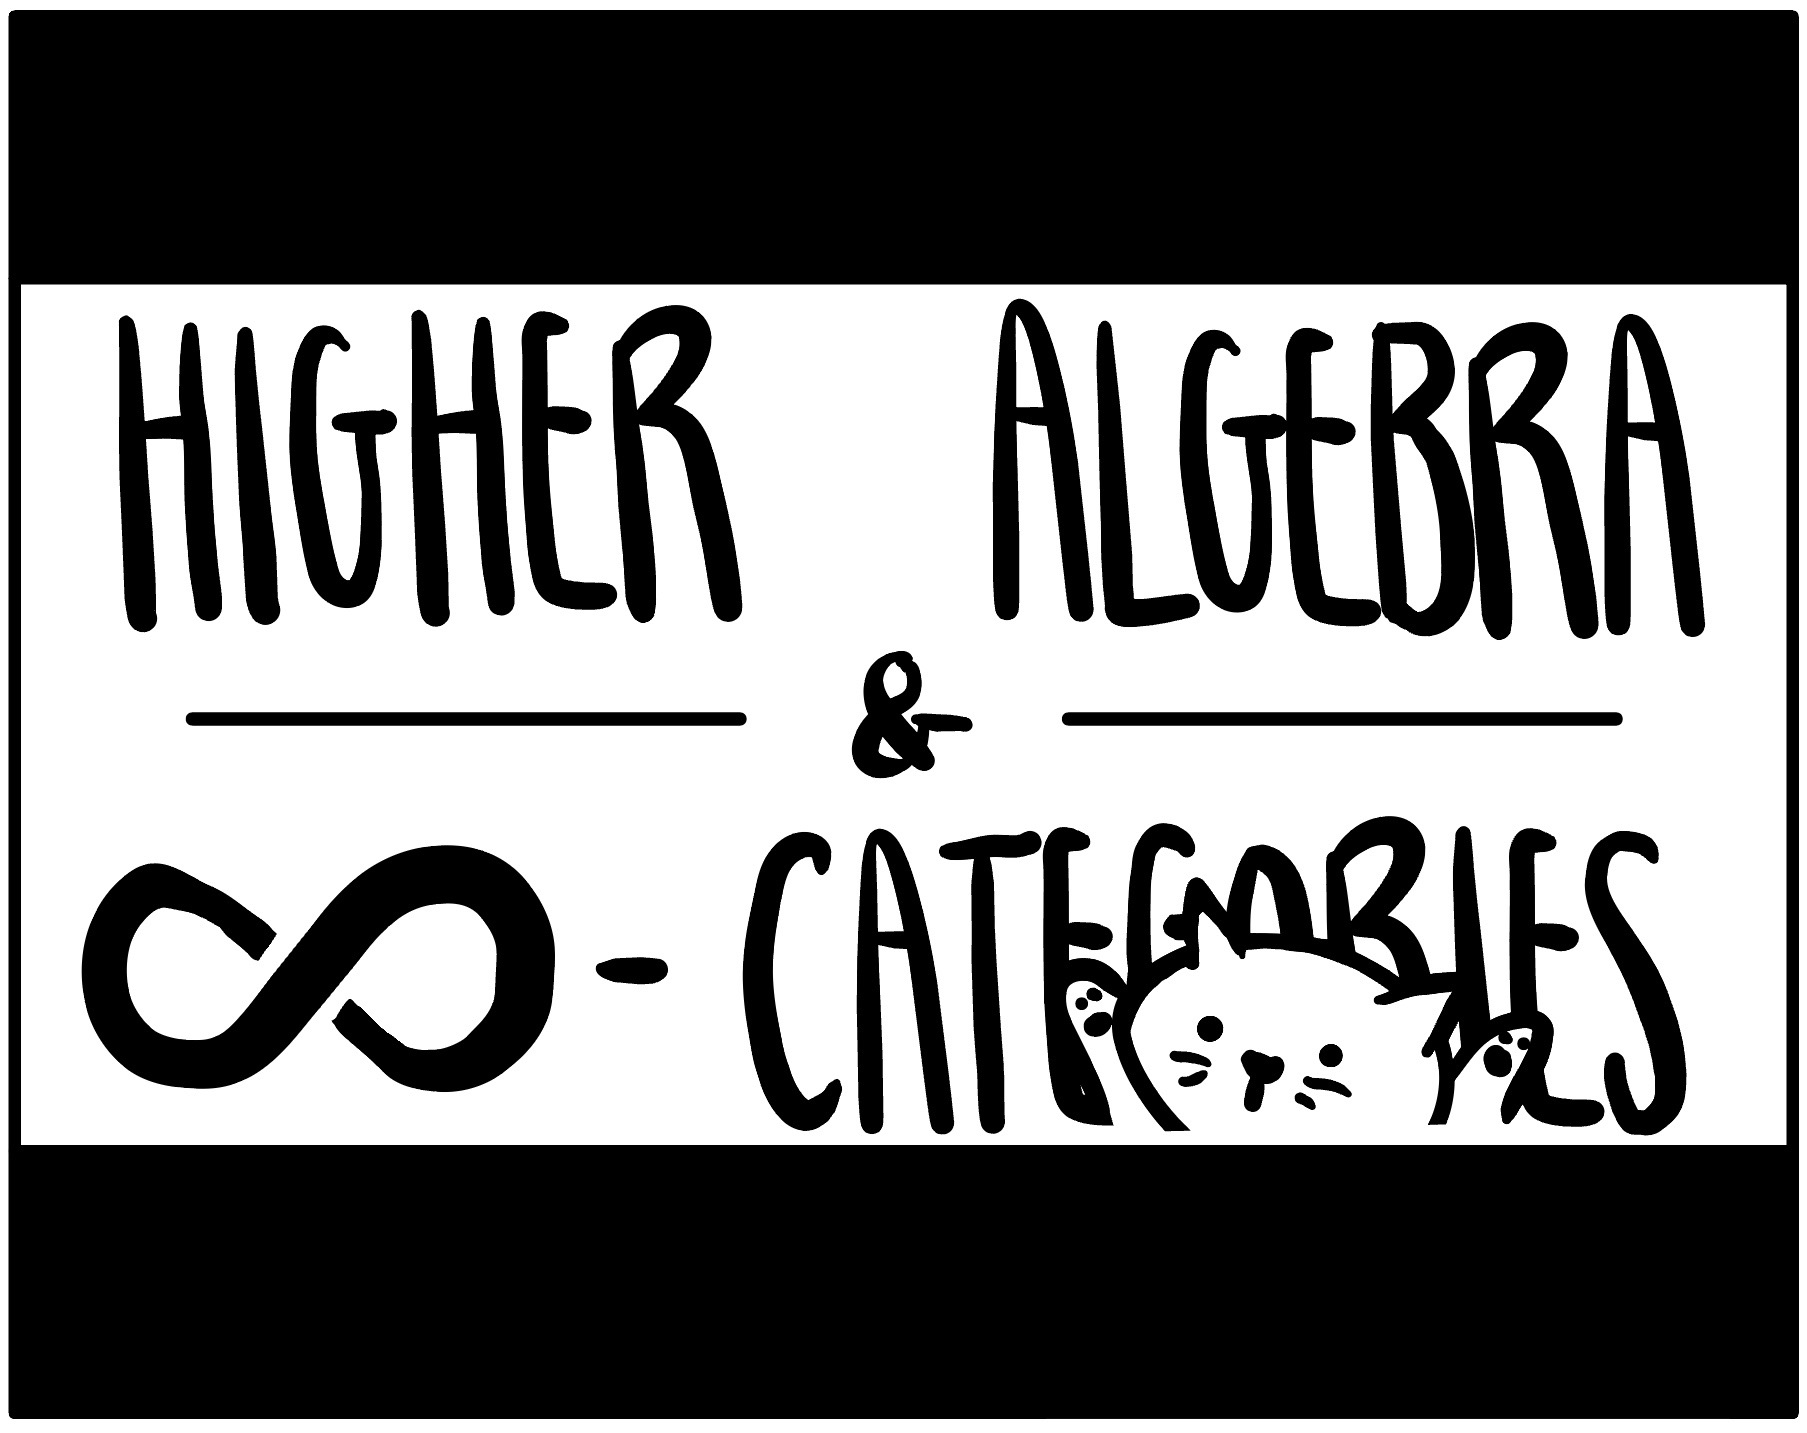
\includegraphics[width=0.5\linewidth]{pics/ha.jpg}
  \centering
  % \caption{}
  % \label{fig:}
\end{figure}

\tableofcontents{}

\section{Lecture 1: Thursday, January 12th}

Today: the \textbf{homotopy hypothesis}

\textbf{Classical algebra}: sets, monoids, groups, abelian groups, rings. Each of these are built up on the other. In higher courses, we may see groupoids, which are types of categories. A category is a generalization of a monoid, in some sense. We also have monoidal categories, which in some sense are a generalization of rings.

For higher algebra: spaces, $\mathbb{E}_1$-spaces, spectra, $\mathbf{E}_1$-ring spectra. Underlying this we have $\infty$-groupoids, $\infty$-categories, and monoidal $\infty$-categories.

We study spaces, not up to homeomorphism, but up to \textit{weak homotopy equivalence}. We will study this in a minute. ``Spaces'' in this class will always mean the study of topological spaces up to weak homotopy equivalence.

We'll give a synthetic definition of what an infinity category is, and circle back to a technical definition in about a month.

\textbf{What is an $\infty$-category}?

An $\infty$-category (or $(\infty,1)$-category) $\mathscr{C}$ should consist of:
\begin{enumerate}
    \item a class of objects
    \item a class of morphisms so that $\Hom_\mathscr{C}(X,Y)$ is a space
    \item $n$-morphisms for $n \ge 2$, where for instance 2-morphisms are between 1-morphisms, 3-morphisms between 2-morphisms, etc.
    \item morphisms can be composed in a suitable way
    \item $n$-morphisms for $n\ge 2$ are invertible in some sense.
\end{enumerate}

An $\infty$-groupoid (or $(\infty,0)$-category) should be an $\infty$-category where all the 1-morphisms are also invertible in some sense.

\textbf{Why study spaces up to weak homotopy equivalence}?

Recall by the Yoneda lemma, we have that
\begin{align*}
    X \cong Y \Leftrightarrow \Hom_\Top(A,X) \cong \Hom_\Top(A,Y)
\end{align*}
for all $A\in \Top$. Figuring out $\Hom(A,X)$ up to bijection for all $A$ is very difficult, so we prefer to study continuous maps up to homotopy. For $X$ and $Y$ nice enough, we say that $f\simeq g$ in $\Hom(X,Y)$ if there exists some path $I \to \Map(X,Y)$ so that $0 \mapsto f$ and $1 \mapsto g$. We define $[X,Y] = \Hom_\Top(X,Y)/\simeq$.

We see then that $X \simeq Y$ if and only if $[A,X] \cong [A,Y]$ for all $A \in \Top$.

We may ask when $[A,-] : \Top_\ast \to \Set$ factors through $\Grp$ or $\Ab$. We have that $[A,-]$ factors through $\Grp$ if and only if $A$ is a co-H-group in $\Top$. That is, we have maps
\begin{align*}
    A &\to A \vee A \\
    A &\to \ast,
\end{align*}
which is coassociative, counital, coinvertible.

\begin{example} $S^n$, when $n \ge 1$, is a co-H-space. The map $S^n \to S^n \vee S^n$ is the pinch map.
\end{example}

We say that $X$ is \textit{weakly homotopy equivalent} to $Y$, we write $X \sim Y$, if and only if there is a map $X \to Y$ inducing an isomorphism 
\[
\pi_n(X) = [S^n,X]_\ast \cong [S^n,Y]_\ast = \pi_n(Y),
\]
for all $n \ge 0$ (for $n \ge 1$ this is a group isomorphism).

If $X \sim Y$, then $H_n(X) \cong H_n(Y)$ for any $n$.

\begin{theorem} (Cellular approximation) For any $X$ in $\Top$, there exists $\til{X}$ a CW complex with a canonical map $\til{X} \xto{\sim} X$ that is a weak equivalence.
\end{theorem}

\begin{theorem} (Whitehead) If $X,Y$ are CW complexes, then $X \xto{\simeq} Y$ is a homotopy equivalence if and only if $X \xto{\sim} Y$ is a weak homotopy equivalence.
\end{theorem}

\begin{exercise} Find spaces $X$ and $Y$ which are weakly homotopy equivalent but not homotopy equivalent.
\end{exercise}

We denote by $\Delta$ the simplex category. Its objects are ordered sets of the form $[n] = \left\{ 0,1, \ldots, n \right\}$, and its morphisms are order-preserving maps. We have that $\Delta$ is generated by \textit{cofaces} and \textit{codegeneracies}. The cofaces are of the form
\begin{align*}
    d^0,d^1: [0] \to [1],
\end{align*}
skipping $0$ or $1$ in $[1]$, etc. The codegeneracies look like $s^0 : [1] \to [0]$ which ``repeat'' an element.

The cofaces and codegeneracies satisfy certain \textit{cosimplicial identities}.

If $\mathscr{C}$ is a category, we denote by $s \mathscr{C} = \mathscr{C}^{\Delta^\op}$ the simplicial objects in $\mathscr{C}$. If $\mathscr{C} = \Set$, we write $\sSet$ as the category of simplicial sets. A simplicial set $X_\bullet \in \sSet$ consists of sets $X_0, X_1, \ldots$ together with face and degeneracy maps satisfying the simplicial identities.

\begin{example} The \textit{nerve of a small category}. Let $\mathscr{C} \in \Cat$ a small category. We denote by $N_\bullet \mathscr{C}$ the simplicial set with $N_0 \mathscr{C} = \ob \mathscr{C}$, $N_1 \mathscr{C} = \mor \mathscr{C}$, and $N_n \mathscr{C}$ the set of $n$ composable morphisms in $\mathscr{C}$. That is,
\begin{align*}
    N_n \mathscr{C} = N_1 \mathscr{C} \times_{N_0 \mathscr{C}} \cdots \times_{N_0 \mathscr{C}} N_1 \mathscr{C}.
\end{align*}
The face maps are source/target/composition. The degeneracies insert an identity morphism.
\end{example}

\begin{example} Via Yoneda, we get a functor
\begin{align*}
    \Delta^n := \Hom_\Delta(-,[n]) : \Delta^\op \to \Set.
\end{align*}
If $X_\bullet$ is a simplicial set, we get that the set of $n$-simplices $X_n$ is in bijection with $\Hom_\sSet(\Delta^n, X_\bullet)$.
\end{example}

\begin{example} (Dold--Kan) We have $\Ch_R^{\ge 0} \xto{\Gamma} s\Mod_R$ is an isomorphism, where $\Gamma_m C_\bullet  =\oplus_{[n] \tto [k]} C_k$, with faces and degeneracies left as an exercise.
\end{example}

\begin{example} Let $\Delta^n_\Top \subseteq \R^{n+1}$ be defined by
\begin{align*}
    \left\{ (t_0, \ldots, t_n) \in \R^{n+1} \colon 0 \le t_i \le 1,\ \sum t_i = 1 \right\}.
\end{align*}
We can view $[n] = \left\{ v_0, \ldots, v_n \right\}$, and $v_i = (0, \ldots, 0,1,0, \ldots, 0)$ with 1 at the $i$th place. Then if $\alpha : [m] \to [n]$ in $\Delta$, we can define $\alpha(v_i) =v_{\alpha(i)}$. Extend linearly to get $\alpha_\ast : \Delta^m_\Top \to \Delta^n_\Top$. We get then that $\Delta^\bullet_\Top$ is a cosimplicial topological space.
\end{example}

\begin{example} If $X \in \Top$, we have $\Sing_\bullet(X) \in \sSet$ defined by $\Sing_n(X) = \Hom_\Top \left( \Delta_\Top^n, X \right)$.
\end{example}

\begin{definition} If $X_\bullet \in \sSet$, we define its \textit{geometric realization} to be
\begin{align*}
    |X_\bullet| = \amalg_{n\ge 0} X_n \times \Delta^n_\Top / \sim,
\end{align*}
where $(x,s)\sim (y,t)$ if and only if there is some $\alpha : [m] \to [n]$ so that $\alpha^\ast y = x$ and $\alpha_\ast s = t$.
\end{definition}


\begin{example} $|\Delta^n_\bullet| \cong \Delta^n_\Top$.
\end{example}

\begin{exercise} $|X_\bullet|$ is always a CW complex for any $X_\bullet \in \sSet$.
\end{exercise}

\begin{exercise} We have an adjunction $|-| : \sSet \rightleftarrows \Top: \Sing(-)$
\end{exercise}

\begin{definition} $X_\bullet \to Y_\bullet$ is a \textit{weak homotopy equivalence} in $\sSet$ if $|X_\bullet| \xto{\sim} |Y_\bullet|$ is a weak homotopy equivalence of spaces.
\end{definition}

\begin{theorem} (Quillen) Simplicial sets up to weak equivalence is equivalent to topological spaces up to weak homotopy equivalence. Moreover, for any $X\in \Top$, we have that $|\Sing(X)|$ is weakly equivalent to $X$.
\end{theorem}

\begin{figure}[h]
  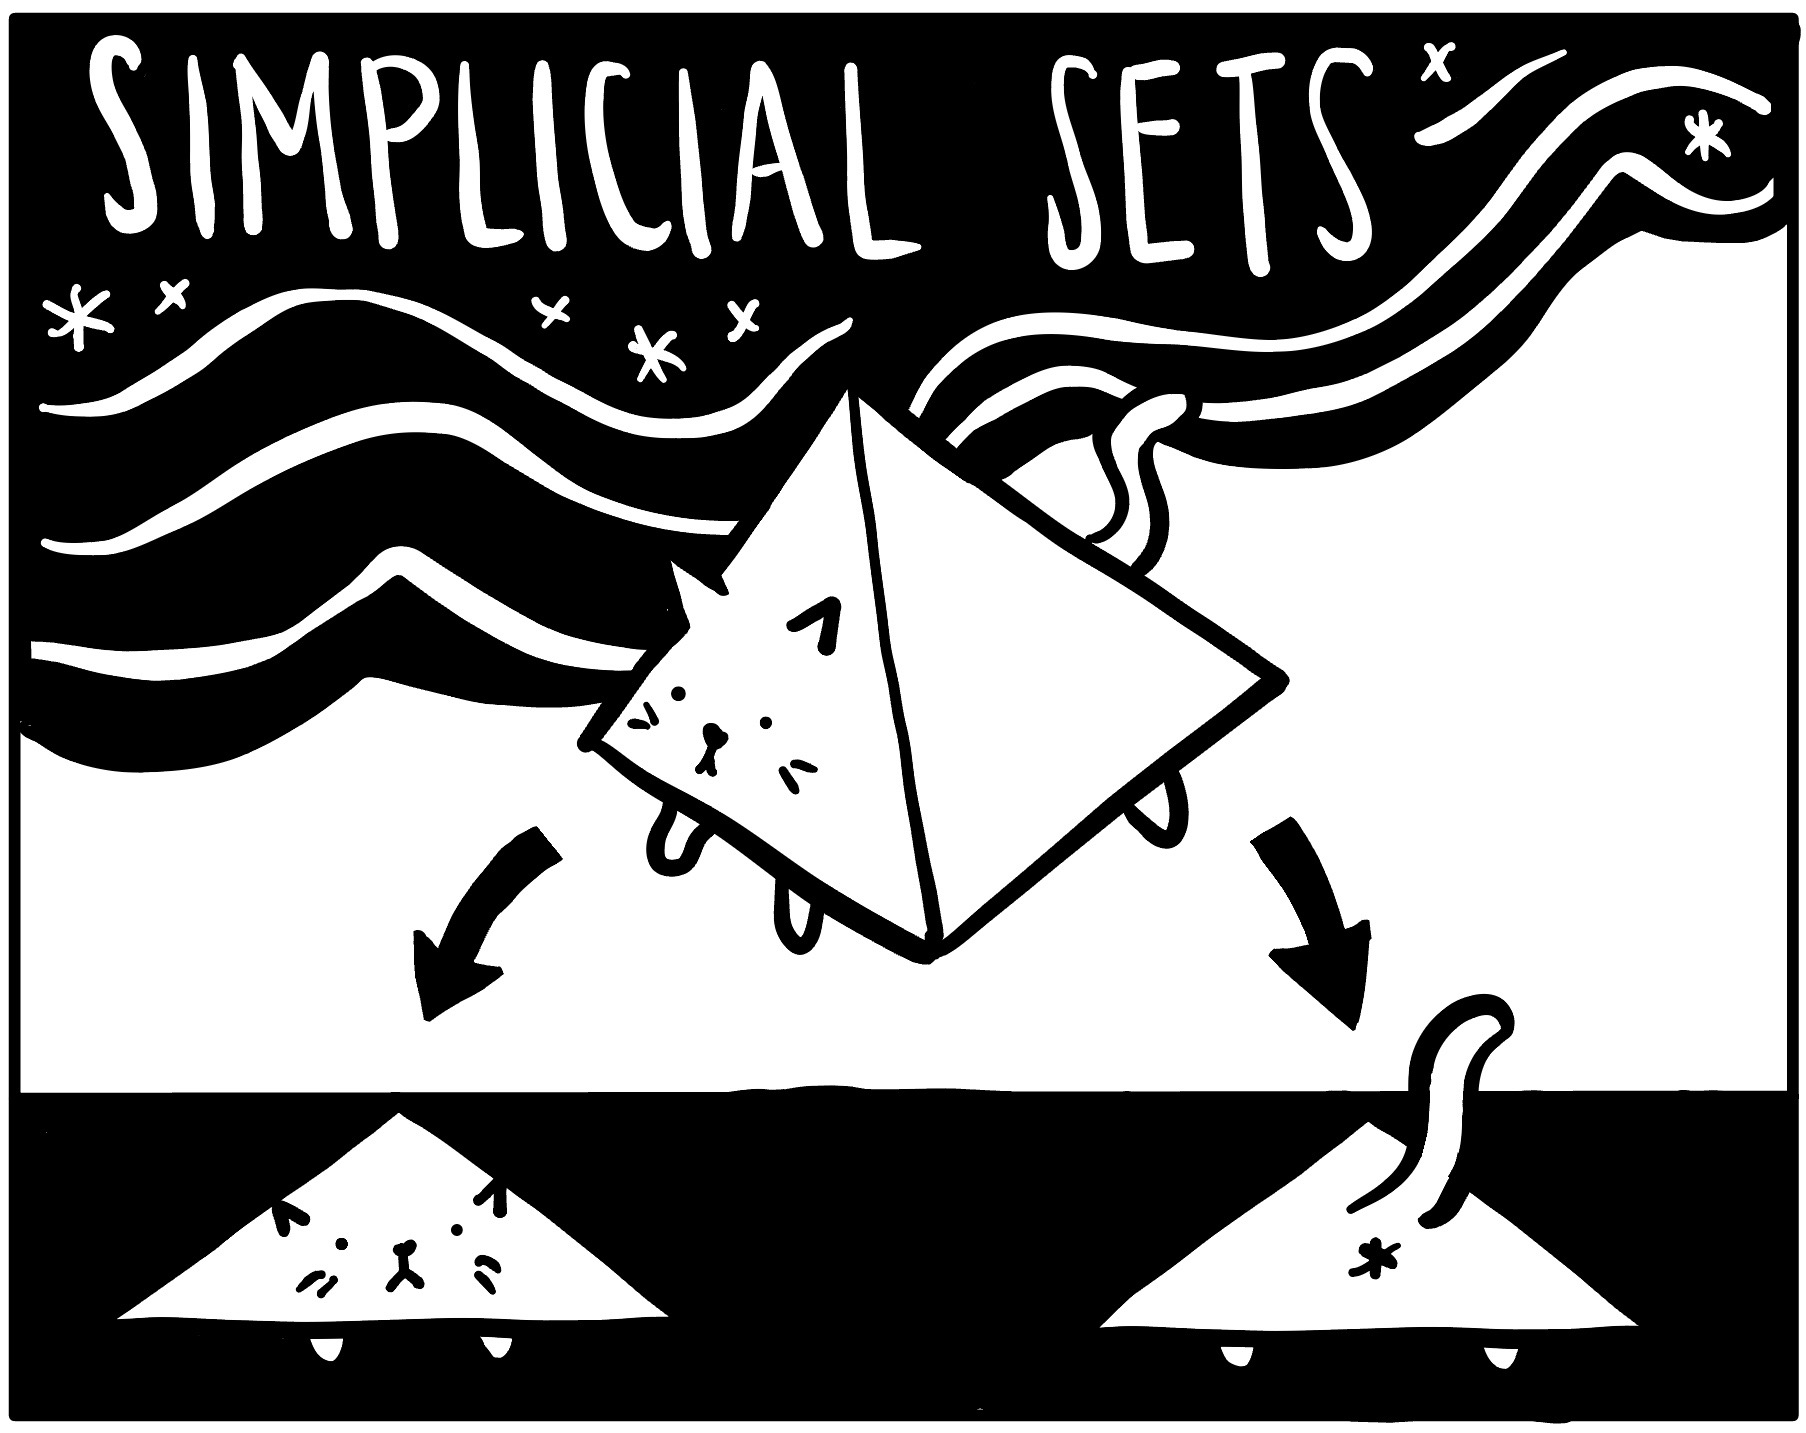
\includegraphics[width=0.5\linewidth]{pics/sset.jpg}
  \centering
 \end{figure}



\section{Lecture 2: Tuesday, January 17th}

\textbf{Today}: the homotopy hypothesis (continued).

Recall we are interested in studying $\Top$ up to weak homotopy equivalences. Equivalently, we are interested in studying $\sSet$ up to weak equivalence, and the relationship between the two was given by the geometric realization / singular complex adjunction.

Recall we've defined $\Delta^n = \Hom_\Delta(-,[n])$. We will define the $k$\textit{th horn} $\Lambda^n_k \subseteq \Delta^n$ as a coequalizer in $\sSet$
\begin{align*}
    \left(\coprod_{0 \le i < j \le n} \Delta^{n-2} \rightrightarrows \coprod_{i\ne k} \Delta^{n-1} \right) \to \Lambda^n_k,
\end{align*}
where the two maps are $\delta^{j-1}$ and $\delta^i$. The geometric realization of $\Lambda^n_k$ is the topological $n$-simplex, with the middle and the face opposite the $k$th edge removed.

\begin{definition} We say that $Y\in \sSet$ is a \textit{Kan complex} if for all $k\le n$, and for every $\Lambda^n_k \to Y$, there exists a (not necessarily unique) lift:
\[ \begin{tikzcd}
    \Lambda^n_k\dar[hook]\rar & Y\\
    \Delta^n\ar[ur,dashed] & 
\end{tikzcd} \]
\end{definition}

\begin{exercise} $Y$ is a Kan complex if and only if for any $(n-1)$-simplices $y_1, \ldots, y_{k-1},y_{k+1}, \ldots, y_n$ such that $d_i y_j = d_{j-1} y_i$ for $i< j$, $i,j\ne k$, there exists an $n$-simplex $y$ such that $d_i y = y_i$ for all $i\ne k$.
\end{exercise}

\begin{exercise} We have that $\Sing(X)$ is always a Kan complex for any $X\in \Top$.
\end{exercise}

\begin{exercise} We have that $\Delta^n$ is not a Kan complex for $n \ge 1$.
\end{exercise}

\begin{exercise} If $X \in s\Grp$, then the underlying simplicial set of $X$ is always a Kan complex.
\end{exercise}

Up to weak homotopy equivalence, every simplicial set is a Kan complex (will see this later).

Recall the Dold-Kan correspondence
\begin{align*}
    s\Mod_\Z \cong \Ch_\Z^{\ge 0},
\end{align*}
which sends weak homotopy equivalences to quasi-isomorphisms. Given a simplicial set $X_\ast$, we can take an associated simplicial abelian group $\Z[X_\ast]$ by taking the free group on $n$-simplices at level $n$. We can ask what $\Z[X_\ast]$ corresponds to as a chain complex. One answer is that
\begin{align*}
    \Z[\Sing(X_\ast)] \leftrightarrow C_\ast(X;\Z).
\end{align*}
This tells us that
\begin{align*}
    \pi_\ast \left( \Z \left[ \Sing(X) \right] \right) \cong H_\ast(X;\Z).
\end{align*}
In some sense we can view $\Z[\Sing(X)]$ as being (equivalent to) the \textit{free commutative monoid} on $X$. This is what is known as the \textit{Dold-Thom theorem}.

\textbf{Homotopy hypothesis}: Spaces (up to weak equivalence) are $\infty$-groupoids. For us, spaces up to weak equivalences correspond to Kan complexes.

Given $X\in \Kan$, we can call $X_0$ the objects, and $X_1$ the morphisms. The horn filling conditions on horns tell you that you can \textit{compose} and \textit{invert} morphisms in $X_1$, witnessed by simplices in $X_2$.

\begin{definition} A \textit{quasi-category} (i.e. $\infty$-category) is a simplicial set with inner horn lifting property. That is, we can lift against horns $\Lambda^n_k$ for $0<k<n$.
\end{definition}

\begin{exercise} A quasi-category has unique horn filling if and only if it is isomorphic to the nerve of a 1-category.
\end{exercise}

\begin{center}
\textbf{Model categories}
\end{center}

\textbf{Vista}: Every nice infinity category is equivalent in some sense to a model category. This will pretty much be the goal of this class.

\begin{notation} Let $\mathcal{M}$ be a category, and $\chi \subseteq \mathcal{M}$ a class of morphisms. We define $\LLP(\chi)$ to be the class of morphisms in $\mathcal{M}$ so that $f$ has left lifting property with respect to all morphisms in $\chi$:
\[\begin{tikzcd}
    \cdot\rar\dar["f" left] & \cdot\dar["\in\ \chi" right]\\
    \cdot\rar\ar[ur,dashed] & \cdot
\end{tikzcd} \]
\end{notation}

Similarly we can define $f\in \RLP(\chi)$ by
\[\begin{tikzcd}
    \cdot\rar\dar["\chi\ \ni" left] & \cdot\dar["f" right]\\
    \cdot\rar\ar[ur,dashed] & \cdot
\end{tikzcd} \]

\begin{figure}[h]
  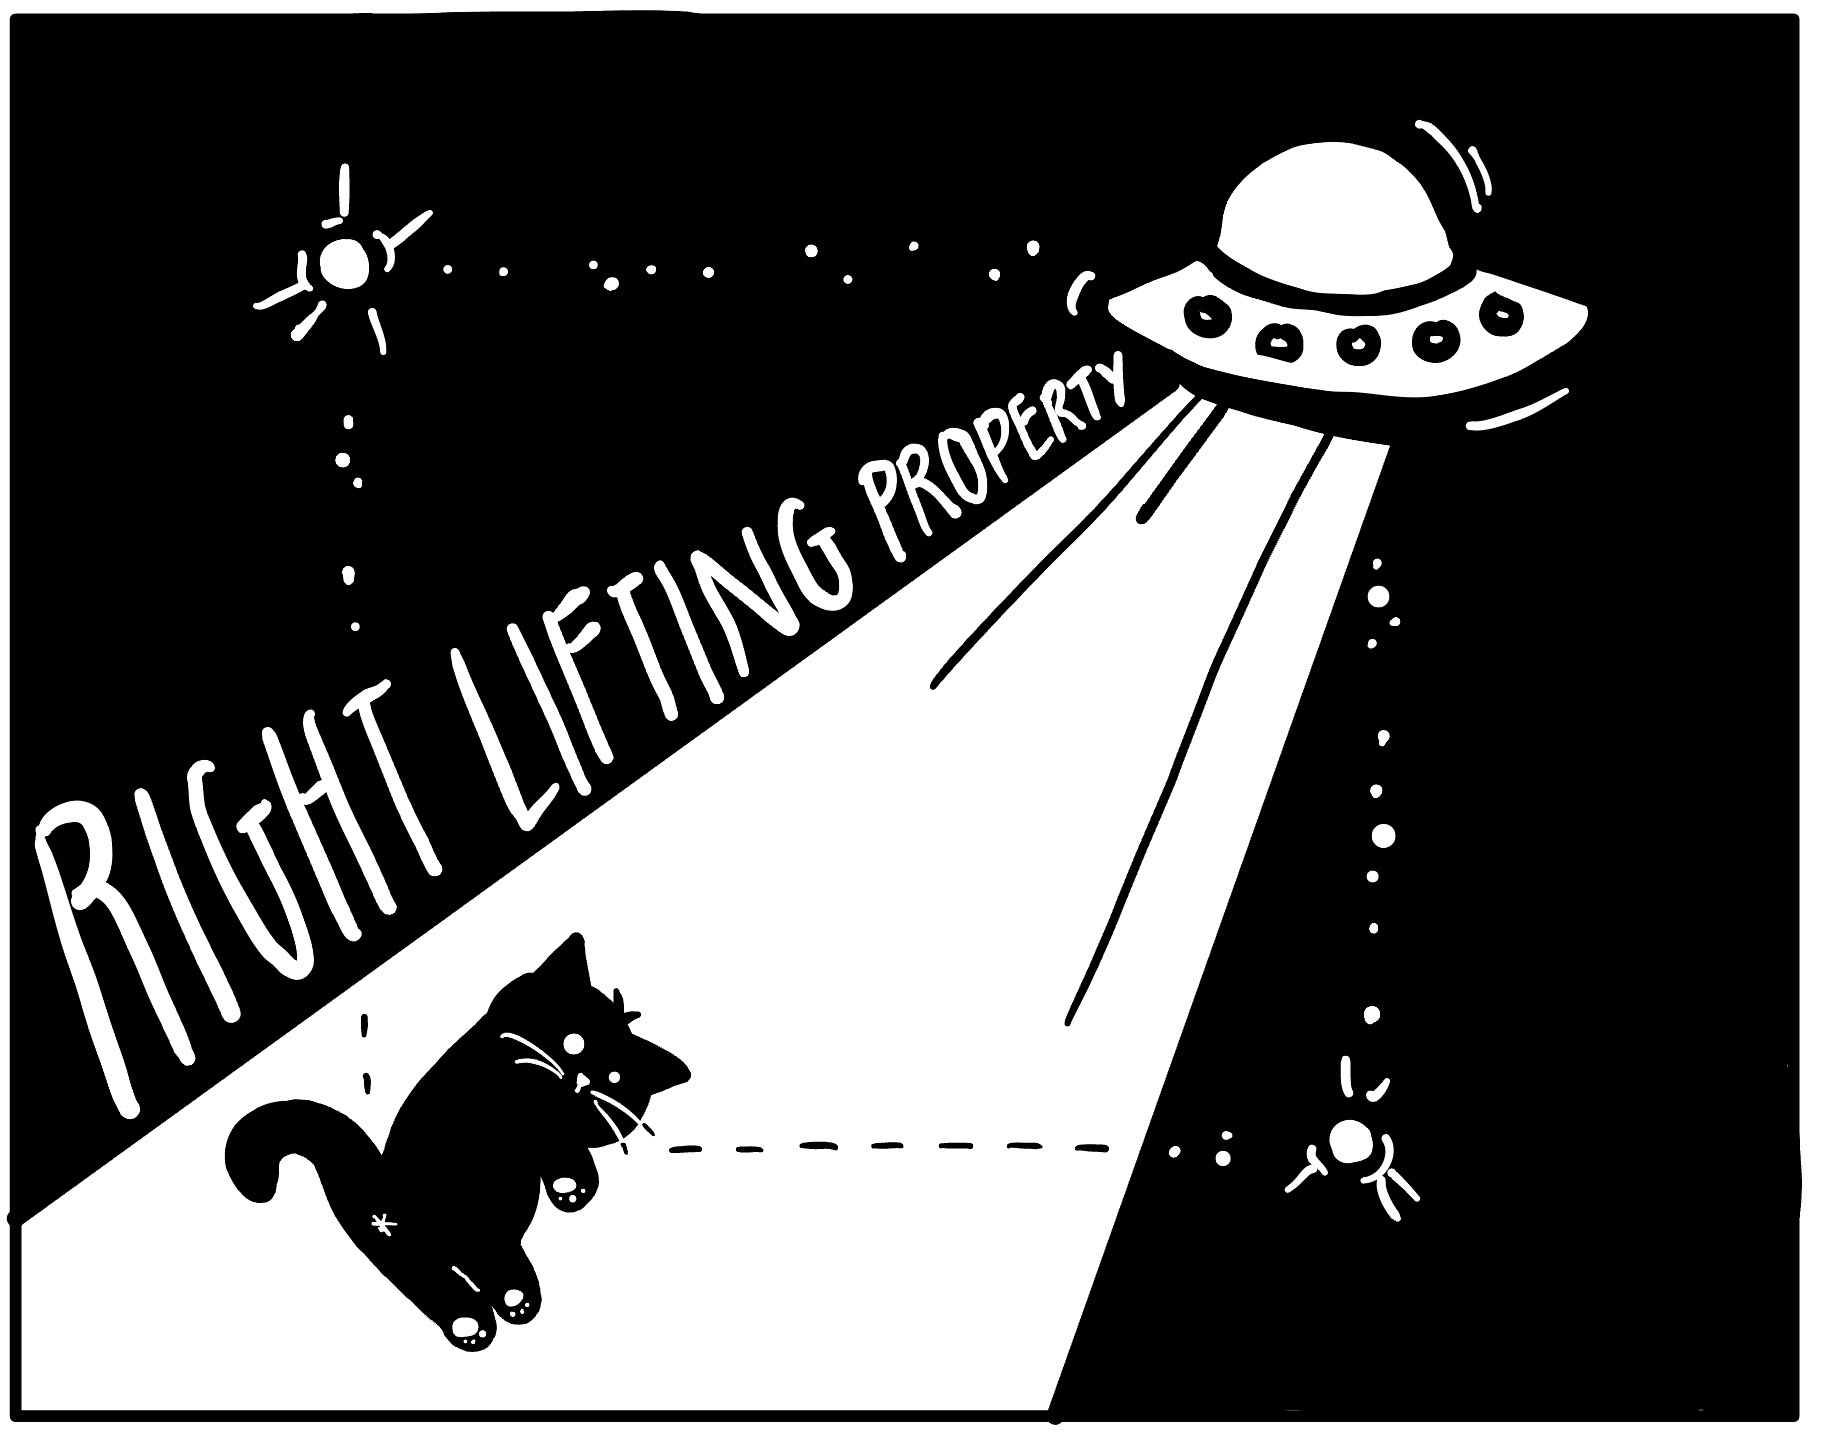
\includegraphics[width=0.5\linewidth]{pics/rlp.jpg}
  \centering
\end{figure}


\begin{definition} A \textit{weak factorization system} on a category $\mathcal{M}$ consists of a pair $(\mathscr{C}, \mathscr{F})$ of classes of morphisms such that
\begin{enumerate}
    \item Given any $f: X \to Y$ in $\mathcal{M}$, it factors (not necessarily uniquely) as
\[ \begin{tikzcd}
    X\ar[rr,"f" above]\ar[dr,"\mathscr{C}\ni" below left] &  & Y\\
     & W\ar[ur,"\in \mathscr{F}" below right] &
\end{tikzcd} \]

    \item $\mathscr{C} = \LLP(\mathscr{F})$ and $\mathscr{F} = \RLP(\mathscr{C})$.
\end{enumerate}
\end{definition}

\begin{example} In $\Set$, we have that mono and epimorphisms give a weak factorization system. A factorization is
\[ \begin{tikzcd}
    X\ar[rr,"f" above]\ar[dr,"\id_X \times f" below left] &  & Y\\
     & X \times Y\ar[ur,"\pi_Y" below right] & 
\end{tikzcd} \]
% The lifting property
% \[ \begin{tikzcd}
%     A\rar\dar[hook] & X\dar[two heads]\\
%     B\rar\ar[ur,dashed] & Y
% \end{tikzcd} \]
\end{example}

\begin{definition} A \textit{model structure} on $\mathcal{M}$ consists of three classes of morphisms:
\begin{center}
    \begin{tabular}{l | l}
    $W$ & weak equivalences \\
    $\Cof$ & cofibrations \\
    $\Fib$ & fibrations
    \end{tabular}
\end{center}
We denote by $\widetilde{\Cof}:= \Cof \cap W$ and $\widetilde{\Fib} = \Fib \cap W$, and call these \textit{trivial cofibrations} (resp. \textit{trivial fibrations}). These are subject to the constraint that
\begin{enumerate}
    \item $\mathcal{M}$ is bicomplete (all limits and colimits)\footnote{We might also require \textit{finitely} bicomplete.}
    \item $W$ satisfies 2-out-of-3 property\footnote{If $f$ and $g$ are composable, and any two of $f$, $g$, $gf$ are in $W$ then so is the third.}
    \item $\left( \Cof, \til{\Fib} \right)$ and $\left( \widetilde{\Cof}, \Fib \right)$ are weak factorization systems.
\end{enumerate}
\end{definition}

\begin{terminology} A category with a model structure is referred to as a \textit{model category}.
\end{terminology}

\begin{figure}[h]
  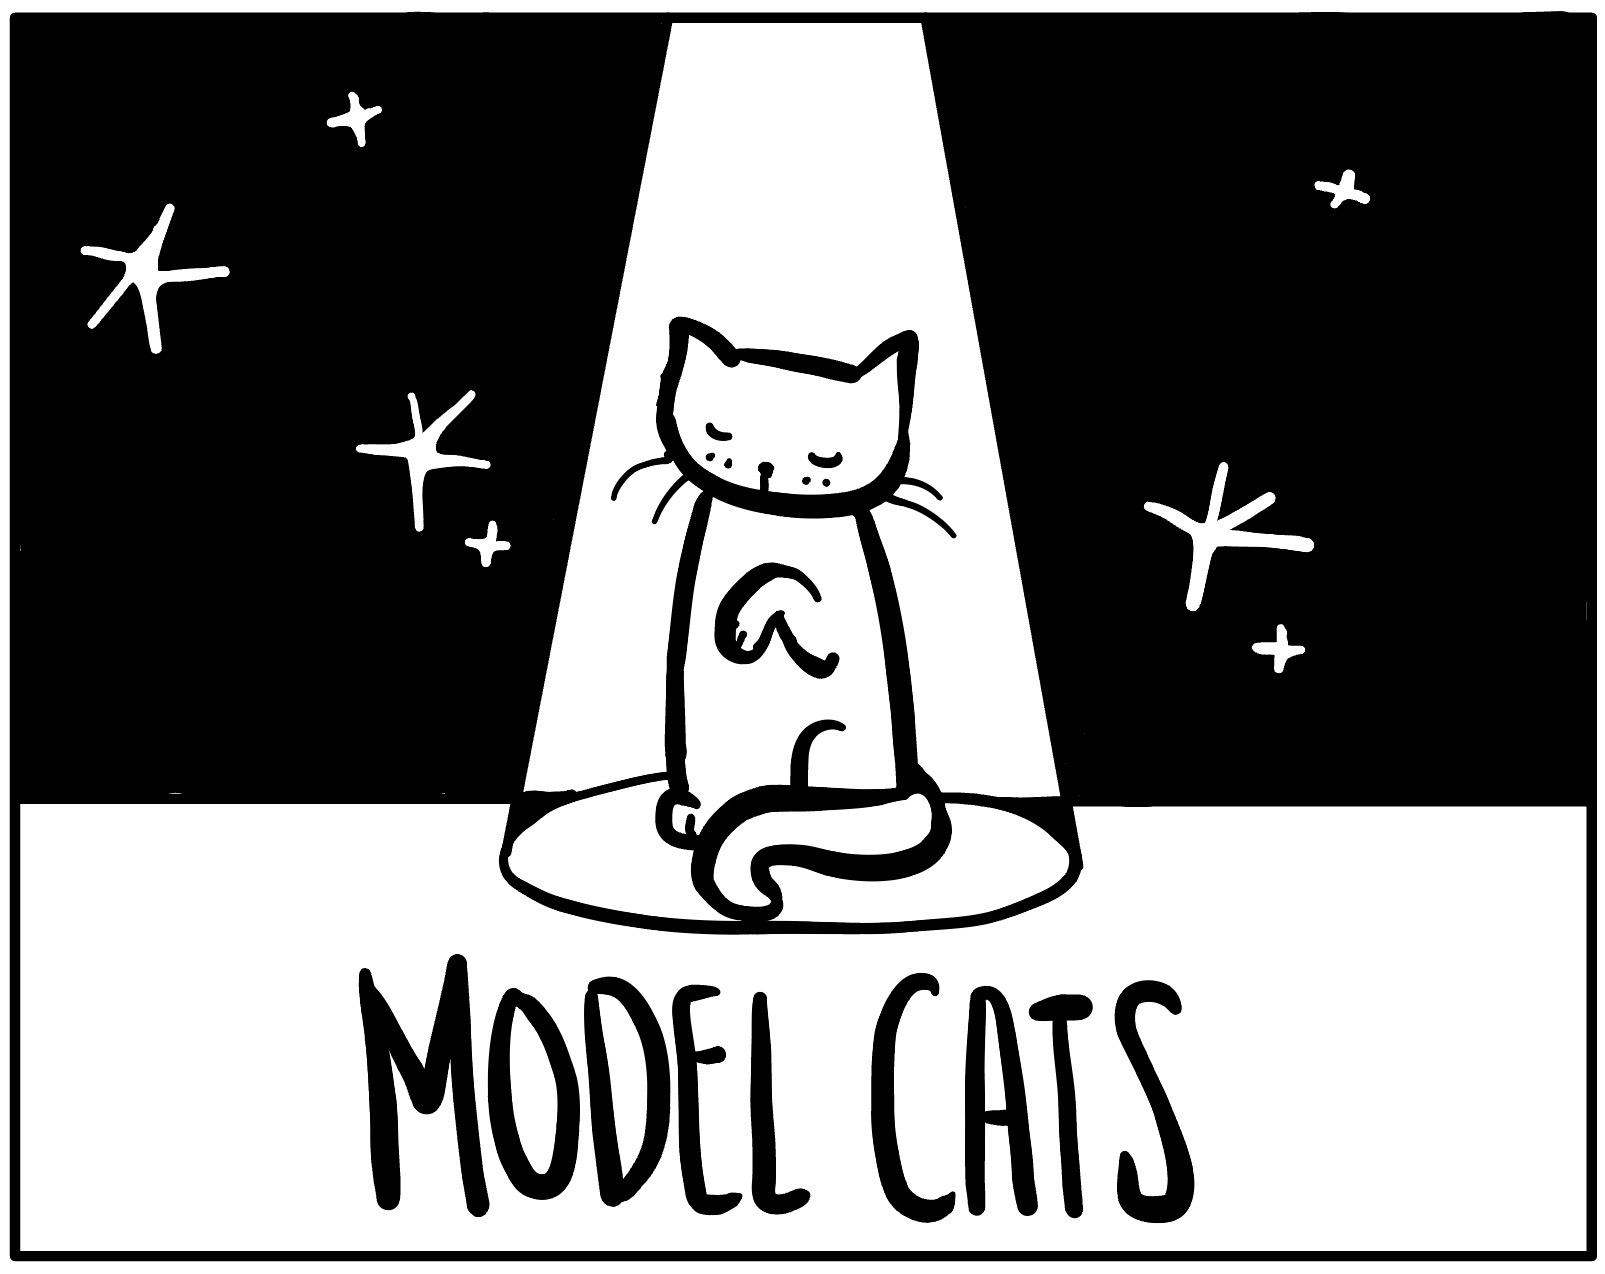
\includegraphics[width=0.5\linewidth]{pics/model-cats.jpg}
  \centering

\end{figure}


\begin{notation} We will decorate each class of morphisms as
\begin{center}
\begin{tabular}{l | l}
    $W$ & $\xto{\sim}$ \\
    $\Cof$ & $\hookto$ \\
    $\Fib$ & $\tto$
    \end{tabular}
\end{center}
\end{notation}


\begin{exercise} $W$, $\Cof$, and $\Fib$ are closed under retracts: that is,
\[ \begin{tikzcd}
    \cdot\dar["f" left]\rar\ar[rr,equal,bend left=20] & \cdot\dar["g"]\rar & \cdot\dar["f"]\\
    \cdot\rar\ar[rr,equal,bend right=20] & \cdot\rar & \cdot\\
\end{tikzcd} \]
then if $g\in W$ (resp. $\Cof$ or $\Fib$) then $f\in W$ (resp. $\Cof$ or $\Fib$).
\end{exercise}

\begin{definition} Let $\mathcal{M}$ be a model category, and let $\emptyset \in \mathcal{M}$ the initial object and $\ast\in \mathcal{M}$ the terminal object. 

\begin{itemize}
    \item We say that $X\in \mathcal{M}$ is \textit{cofibrant} if the unique map $\emptyset \to X$ is a cofibration. 
    \item We say that $X\in \mathcal{M}$ is \textit{fibrant} if the unique map $X \to \ast$ is a fibration.
    \item We say that $\til{X}$ is a \textit{cofibrant replacement} of $X$ if
\[ \begin{tikzcd}
    \emptyset\ar[rr]\ar[dr,hook] &  & X\\
     & \til{X}\ar[ur,two heads,"\sim" below right] & 
\end{tikzcd} \]
    \item We say that $\til{X}$ is a \textit{fibrant replacement} of $X$ if
\[ \begin{tikzcd}
    X\ar[rr]\ar[dr,hook,"\sim" below left] &  & \ast\\
     & \til{X}\ar[ur,two heads] & 
\end{tikzcd} \]
\end{itemize}
\end{definition}

\begin{example} $\mathcal{M} = \Top$, $W=$ weak homotopy equivalences, $\Cof=$ relative CW complexes\footnote{$A\hookto X$ is a \textit{relative CW complex} if $X$ is built out of $A$ by attaching cells.} The fibrations are determined by $\Fib = \RLP(\widetilde{\Cof})$. The fibrations are equivalently $\RLP(D^n \to D^n \times I)$. Every object here is fibrant, and the cofibrant objects are precisely the CW complexes. Cofibrant replacement is cellular approximation.
\end{example}

\section{Lecture 3: Thursday, January 19th}

\begin{proposition}\label{prop:labelname} Identities and isomorphisms are weak equivalences in a model category.
\end{proposition}
\begin{proof} For any $X \in \mathcal{M}$, we can fibrantly replace it to get $X \xhookto{\sim} \til{X}$. Consider the commutative diagram
\[ \begin{tikzcd}
    X\ar[rr,"\id"]\ar[dr,hook,"\sim" below left] &  & X\ar[dl,"\sim" below right]\\
     & \til{X}. & 
\end{tikzcd} \]
By 2-out-of-3, we have that $\id:X \to X$ is also a weak equivalence.

More generally if $f:X \to Y$ is an isomorphism in $\mathcal{M}$, then by the diagram
\[ \begin{tikzcd}
    X\dar["f" left]\rar["f" above]\ar[rr,equal,bend left=20] & Y\dar[equal]\rar["f^{-1}"] & X\dar["f" right]\\
    Y\rar[equal] & Y\rar[equal] & Y,
\end{tikzcd} \]
we see that $f$ is contained in $W$.
\end{proof}

If $\left( \mathscr{C},\mathscr{F} \right)$ is a weak factorization system, then both $\mathscr{C}$ and $\mathscr{F}$ are closed under retracts. Hence $\Cof, \til{\Cof}, \Fib, \til{\Fib}$ are closed under retracts. $W$ is also closed under retracts (exercise).

\begin{exercise} We have that $\mathcal{M}$ is a model category if and only if $\mathcal{M}^\op$ is a model category.
\end{exercise}

\begin{theorem} Cofibrations are closed under pushouts and coproducts.
\end{theorem}
\begin{proof} Given any test square, we can try to lift:
\[\begin{tikzcd}
    X\rar\dar[hook] & Y\rar\dar & A\dar[two heads,"\sim" right]\\
    Z\rar\ar[urr,dashed] & P\rar\po & B.
\end{tikzcd} \]
This map is constructed by universal property of the pushout:
\[ \begin{tikzcd}
    X\rar\dar[hook] & Y\dar\ar[ddr,bend left=10] & \\
    Z\rar\ar[drr,bend right=10,dashed] & P\po\ar[dr,dashed,"\exists!" above right] & \\
     &  & A.
\end{tikzcd} \]
For coproducts, we can take $X_i \hookto Y_i$ for $i\in J$. Let's try to lift:
\[ \begin{tikzcd}
    X_i\dar[hook]\rar & \amalg_i X_i\dar\rar & A\dar[two heads,"\sim" right]\\
    Y_i\rar\ar[urr,dashed] & \amalg_i Y_i\rar & B.
\end{tikzcd} \]
We know that each $X_i\hookto Y_i$ is a cofibration hence it lifts against the big square. By universal property a map $\amalg_i Y_i \to A$ exists.
\end{proof}


\begin{example} If $\mathscr{C}$ is a bicomplete category, then $\mathscr{C}$ has a model structure where $W$ is the isomorphisms, and $\Cof = \Fib = \mor \mathscr{C}$.
\end{example}

\begin{example} If $\mathcal{M} = \Top$, we have the \textit{Quillen model structure}, with
\begin{itemize}
    \item $W=$ weak homotopy equivalences
    \item $\Cof=$ retracts of relative CW complexes
    \item $\Fib=$ Serre fibrations ($\RLP(D^n \hookto D^n \times I)$).
\end{itemize}
\end{example}


\begin{example} The Str{\o}m (or Hurewicz) model structure on $\Top$:
\begin{itemize}
    \item $W=$ homotopy equivalences
    \item $\Fib=$ Hurewicz fibrations ($\RLP(A \to A \times I)$ for all $A \in \Top$)
    \item $\Cof=$ closed cofibrations in $\Top$.
\end{itemize}
Fibrant replacement in the Str{\o}m model structure looks like
\[ \begin{tikzcd}
    X\ar[rr,"f"]\ar[dr,hook] &  & Y\\
     & M_f\ar[ur,two heads,"\simeq" below right] &
\end{tikzcd} \]
Where $M_f = (X \times I)\cup_X Y$ is the mapping cylinder.
\end{example}

\begin{example} The \textit{Kan model structure} on $\sSet$ with
\begin{itemize}
    \item $W=$ weak homotopy equivalences
    \item $\Cof=$ monomorphisms (levelwise injections)
    \item $\Fib=$ Kan fibrations ($\RLP(\Lambda_k^n \to \Delta^n)$ for all $0\le k\le n$).
\end{itemize}
Everything is cofibrant here (since the empty simplicial set injects into everything). Fibrant things are Kan complexes. This tells us that every simplicial set is weakly equivalent to a Kan complex!
\end{example}

\begin{theorem} (Milnor) The natural map $X \to \Sing(|X|)$ is a weak homotopy equivalence for any simplicial set $X$. [Kerodon, 3.5.4.1]
\end{theorem}


\begin{definition} Let $\mathscr{C}$ be a cat, and $W \subseteq \mathscr{C}$ a subcategory. A functor $F: \mathscr{C} \to \mathscr{D}$ is called the \textit{localization of $\mathscr{C}$ with respect to $W$} if:
\begin{enumerate}
    \item $F(f) \in \text{iso} \mathscr{D}$ if $f\in \mor W$
    \item For any other $F'$ satisfying (1), we have
\[ \begin{tikzcd}
    \mathscr{C}\rar["F'"]\dar["F" left] & \mathscr{D}'\\
    \mathscr{C}\ar[ur,"\exists!" below right] & 
\end{tikzcd} \]
\end{enumerate}
We denote by $\mathscr{C} \to \mathscr{C}[W^{-1}]$ the localization.
\end{definition}

Here is a naive way to construct $\mathscr{C}[W^{-1}]$: we take the free category on $\mathscr{C}$ and ``$W^{-1}$.'' That is, we take the same objects, but allow morphisms to be ``zigzags'' of morphisms forward in $\mathscr{C}$ and morphisms backwards in $W$, and we mod out by the relation that things in $W$ become isomorphisms. There are size issues here.

\begin{theorem} If $\mathcal{M}$ is a model category, then localization $\mathcal{M} \to \mathcal{M}[W^{-1}]$ exists. We denote by $\Ho(\mathcal{M}) = \mathcal{M}[W^{-1}]$ the homotopy category of $\mathcal{M}$.
\end{theorem}

Recall in $\Top$ that $f \simeq g : X \to Y$ if there is a map $H: X \times I \to Y$ so that $H(-,0) = f$ and $H(-,1) = g$. 

\begin{definition} Le t$\mathcal{M}$ be a model category. A \textit{cylinder object} on $X\in \mathcal{M}$ is defined to be
\[ \begin{tikzcd}
    X\amalg X\ar[rr,"\nabla"]\ar[dr,hook] &  & Y\\
     & \Cyl(X)\ar[ur,"\sim" below right] &
\end{tikzcd} \]
The construction of cylinder objects is \textit{not functorial}.
\end{definition}

A \textit{(left) homotopy} from $f$ to $g$ is a map $H: \Cyl(X) \to Y$ such that $H\circ i_0 = f$ and $H\circ i_1 = g$. We denote this by $f\simeq g$.

\begin{proposition} We have that $i_0 : X \to \Cyl(X)$ is a weak equivalence (and same for $i_1$).
\end{proposition}
\begin{proof} We have
\[\begin{tikzcd}
    X\ar[rr,"\id", bend left=30]\ar[dr,dashed,"i_0" below left]\rar & X\amalg X\rar["\nabla"]\dar & Y\\
     & \Cyl(X)\ar[ur,"\sim" below right] & \\
\end{tikzcd} \]
By 2-out-of-3 on the outside maps, the result follows.
\end{proof}

\begin{proposition} If $X$ is cofibrant, then $i_0,i_1: X \to \Cyl(X)$ are cofibrations.
\end{proposition}
\begin{proof} Since cofibrations are preserved under pushouts, we have that $i_0$ and $i_1$ are cofibrations:
\[ \begin{tikzcd}
    \emptyset\rar[hook]\dar[hook] & X\dar["i_0" right]\\
    X\rar["i_1" below] & X \amalg X \po
\end{tikzcd} \]
\end{proof}

\begin{theorem} (Exercise) If $X$ is cofibrant, then homotopy $\simeq$ gives an equivalence relation on $\Hom(X,Y)$ for any $Y$.
\end{theorem}

We can think of a map
\begin{align*}
    \Hom_\mathcal{M}(X,Y)/\simeq \times \Hom_\mathcal{M}(Y,Z)/\simeq &\to \Hom_\mathcal{M}(X,Z)/\simeq \\
    (f,g) &\mapsto g\circ f.
\end{align*}
In order for this to be well-defined, we need $Z$ to be fibrant.

\begin{lemma} If $Z$ is fibrant, and $f\simeq g: X \to Z$, then if $h: X' \to X$, we have that $fh\simeq gh$.
\end{lemma}
\begin{proof} We have $H: \Cyl(X) \to Y$ with $H_0 = f$ and $H_1 = g$. By lifting, we get
\[ \begin{tikzcd}
    X'\amalg X'\rar\dar[hook] & X\amalg X\rar & \Cyl(X)\dar[two heads,"\sim" right]\\
    \Cyl(X')\rar\ar[urr,dashed] & X'\rar & X.
\end{tikzcd} \]
This gives the desired map. We used fibrancy of $Z$ to ensure that the map $\Cyl(X) \to X$ was a trivial fibration (or could be replaced with a better cylinder object using a map to $Z$).
\end{proof}

\begin{theorem} In $\mathcal{M}$, given $f: X \to Y$ with $X$ cofibrant and $Y$ fibrant, then $f\in W$ if and only if $f$ is a homotopy equivalence.\footnote{Meaning that there is some $g: Y \to X$ with $fg\simeq \id$ and $gf\simeq \id$.}
\end{theorem}

\begin{notation} $\mathcal{M}_c=$ cofibrant objects in $\mathcal{M}$, and $\mathcal{M}_f=$ fibrant objects in $\mathcal{M}$. We denote by $\mathcal{M}_{cf}=$ objects which are \textit{both} cofibrant and fibrant.
\end{notation}

Concretely, we can define $\Ho(\mathcal{M})$ as the objects in $\mathcal{M}$, but where
\begin{align*}
    \Hom_{\Ho(\mathcal{M})}(X,Y) = \Hom_{\mathcal{M}_{cf}/\simeq}(RQX,RQY),
\end{align*}
where $R$ is a fibrant replacement and $Q$ is a cofibrant replacement.

\begin{exercise} Given $X \to Y$ in $\mathcal{M}$, there exists $QX \xto{\til{f}} QY$ such that
\[ \begin{tikzcd}
    QX\dar[two heads,"\sim"]\rar["\til{f}"] & QY\dar[two heads,"\sim"]\\
    X\rar["f" below] & Y.
\end{tikzcd} \]
Here $\til{f}$ is well-defined up to left homotopy.
\end{exercise}

Given some $\mathcal{M} \to \Ho(\mathcal{M})$, we just need to check that $W \mapsto$ isos, and it is universal in that way.

\section{Lecture 4: Tuesday, January 24th}

\begin{definition} Suppose $\mathcal{M}$ and $\mathcal{N}$ are model categories, and take a functor $F: \mathcal{M} \to \mathcal{N}$. A \textit{left derived functor} of $F$ is an (absolute) right Kan extension of $F$ along $\gamma_\mathcal{M} : \mathcal{M} \to \Ho(\mathcal{M})$:
% https://q.uiver.app/?q=WzAsMyxbMCwwLCJcXG1hdGhjYWx7TX0iXSxbMSwwLCJcXG1hdGhjYWx7Tn0iXSxbMCwxLCJcXEhvKFxcbWF0aGNhbHtNfSkiXSxbMCwxLCJGIl0sWzAsMiwiXFxnYW1tYV9cXG1hdGhjYWx7TX0iLDJdLFsyLDEsIiIsMix7ImN1cnZlIjoyLCJzdHlsZSI6eyJib2R5Ijp7Im5hbWUiOiJkYXNoZWQifX19XSxbNSwwLCJcXGVsbCIsMix7InNob3J0ZW4iOnsic291cmNlIjoyMH19XV0=
\[\begin{tikzcd}
	{\mathcal{M}} & {\mathcal{N}} \\
	{\Ho(\mathcal{M})}
	\arrow["F", from=1-1, to=1-2]
	\arrow["{\gamma_\mathcal{M}}"', from=1-1, to=2-1]
	\arrow[""{name=0, anchor=center, inner sep=0}, curve={height=12pt}, dashed, from=2-1, to=1-2]
	\arrow["\ell"', shorten <=5pt, Rightarrow, from=0, to=1-1]
\end{tikzcd}\]
if $G: \Ho(\mathcal{M}) \to \mathcal{N}$ and $s: G\circ \gamma_\mathcal{M} \Rightarrow F$, then there exists a unique $s': G\Rightarrow LF$ so that $\ell\circ (s'\circ \gamma_{\mathcal{M}}) = s$.
% https://q.uiver.app/?q=WzAsMyxbMCwwLCJcXG1hdGhjYWx7TX0iXSxbMSwwLCJcXG1hdGhjYWx7Tn0iXSxbMCwxLCJcXEhvKFxcbWF0aGNhbHtNfSkiXSxbMCwxLCJGIl0sWzAsMiwiXFxnYW1tYV9cXG1hdGhjYWx7TX0iLDJdLFsyLDEsIiIsMix7InN0eWxlIjp7ImJvZHkiOnsibmFtZSI6ImRhc2hlZCJ9fX1dLFsyLDEsIiIsMSx7ImN1cnZlIjoyfV0sWzUsMCwiXFxlbGwiLDIseyJzaG9ydGVuIjp7InNvdXJjZSI6MjB9fV0sWzYsNSwicyciLDIseyJzaG9ydGVuIjp7InNvdXJjZSI6MjAsInRhcmdldCI6MjB9fV1d
\[\begin{tikzcd}
	{\mathcal{M}} & {\mathcal{N}} \\
	{\Ho(\mathcal{M})}
	\arrow["F", from=1-1, to=1-2]
	\arrow["{\gamma_\mathcal{M}}"', from=1-1, to=2-1]
	\arrow[""{name=0, anchor=center, inner sep=0}, dashed, from=2-1, to=1-2]
	\arrow[""{name=1, anchor=center, inner sep=0}, curve={height=12pt}, from=2-1, to=1-2]
	\arrow["\ell"', shorten <=3pt, Rightarrow, from=0, to=1-1]
	\arrow["{s'}"', shorten <=2pt, shorten >=2pt, Rightarrow, from=1, to=0]
\end{tikzcd}\]
\end{definition}

\begin{definition} Let $F: \mathcal{M} \to \mathcal{N}$. A \textit{total left derived functor} $\mathbb{L}F: \Ho(\mathcal{M}) \to \Ho(\mathcal{N})$ is the left derived functor of $\mathcal{M} \xto{F} \mathcal{N} \xto{\gamma_\mathcal{N}} \Ho(\mathcal{N})$.
\end{definition}


\begin{example} If $\mathcal{F}: \mathcal{M} \to \mathcal{N}$ where if $f\in W$ between cofibrant objects then $Ff$ is a weak equivalence in $\mathcal{N}$, then $\mathbb{L}F$ exists:
\[ \begin{tikzcd}
    \mathcal{M}\rar["F"]\dar & \mathcal{N}\rar & \Ho(\mathcal{N})\\
    \Ho(\mathcal{M})\ar[urr,bend right=10,dashed] &  & 
\end{tikzcd} \]
\end{example}

We will have that $\mathbb{L}F(X) \xto{\sim} F(X)$ whenever $X$ is cofibrant. In general, $\mathbb{L}F(X) = F(Q(X))$.

\begin{definition} Let $F: \mathcal{M} \to \mathcal{N}$. We say that $F$ is a \textit{left Quillen functor} if
\begin{enumerate}[(i)]
    \item $F$ is a left adjoint
    \item $F$ preserves cofibrations and trivial cofibrations.
\end{enumerate}
In this case if $G$ is a right adjoint, then we say the adjunction is a \textit{Quillen adjunction / Quillen pair}.\footnote{There is a dual notion of right Quillen functor, meaning it is a right adjoint which preserves fibrations and trivial fibrations.}
\end{definition}

\begin{exercise} Show that $L$ is left Quillen if and only if $G$ is right Quillen.
\end{exercise}

\begin{lemma} (Ken Brown's Lemma) If $F: \mathcal{M} \to \mathcal{N}$ is any functor between model categories which sends trivial cofibrations between cofibrant objects to weak equivalences in $\mathcal{N}$, then $F$ sends any weak equivalence between cofibrant objects to weak equivalences.
\end{lemma}
\begin{proof} Let $f: A \xto{\sim} B$, where $A,B \in \mathcal{M}_c$. We need $F(f)$ to be a weak equivalence. Consider the factorization of the coproduct of $f$ and the identity on $B$:
\[ \begin{tikzcd}
    A\amalg B\ar[rr,"f\amalg \id_B"]\ar[dr,hook,"q" below left] &  & B\\
     & C\ar[ur,"\sim" above left,"p" below right,two heads] &
\end{tikzcd} \]
Then consider the pushout:
\[ \begin{tikzcd}
    \emptyset\rar[hook]\dar[hook] & A\dar[hook,"i_A"]\rar["f"]\ar[ddr,"\sim"] & B & \\
    B\rar[hook]\ar[drr,"q"]\ar[ddrr,equal] & A\amalg B\ar[dr,"q"] &  & \\
     &  & C\dar["p"]\ar[uu,"p"] & \\
     &  & B & \\
\end{tikzcd} \]
We have that
\begin{align*}
    B \xhookto{i_B} A\amalg B \xhookto{q} C \\
    A \xhookto{i_A} A\amalg B \xhookto{q} C 
\end{align*}
are both trivial cofibrations, hence their images under $F$ are weak equivalences. We see that
\begin{align*}
    F(p)\circ F(q\circ \id_B) = F(p\circ q\circ \id_B) = F(\id_B).
\end{align*}
Therefore $F(p)$ is a weak equivalence by 2-out-of-3.
\end{proof}

\begin{theorem} Suppose that $F:\mathcal{M}\to \mathcal{M}$ is left Quillen. Then $\mathbb{L}F:\Ho(\mathcal{M})\to \Ho(\mathcal{N})$ exists and can be defined as
\begin{align*}
    \Ho(\mathcal{M})\xto{Q} \Ho(\mathcal{M}_c) \xto{F} \Ho(\mathcal{N}).
\end{align*}
Moreover, we obtain an adjunction on the homotopy categories:
\begin{align*}
    \mathbb{L}F: \Ho(\mathcal{M}) \rightleftarrows \Ho(\mathcal{N}): \mathbb{R}G.
\end{align*}
\end{theorem}
\begin{proof}[Proof idea] We have a natural iso
\begin{align*}
    \Hom_\mathcal{M}(X,G(Y)) \cong \Hom_\mathcal{N}(F(X),Y),
\end{align*}
compatible with homotopy equivalence:
\begin{align*}
    \Hom_\mathcal{M}(X,G(Y))/\simeq \cong \Hom_\mathcal{N}(F(X),Y)/\simeq
\end{align*}
\end{proof}

\textbf{Theorem/Definition:} Take a Quillen adjunction $F: \mathcal{M} \rightleftarrows \mathcal{N}: G$. Suppose that $f: X \xto{\sim} G(Y)$, with $X\in \mathcal{M}_c$ and $Y\in \mathcal{N}_f$ is a weak equivalence if and only if $f^\flat:F(X) \to Y$ is. Then $\mathbb{L}F$ and $\mathbb{R}G$ are equivalences of categories, we call this a \textit{Quillen equivalence}.

\begin{example} We have that
\begin{align*}
    |-|:\sSet_\text{Kan} \rightleftarrows \Top_\text{Quillen}: \Sing(-)
\end{align*}
is a Quillen equivalence.
\end{example}

\begin{example} We have that
\begin{align*}
    \id: \Top_\text{Quillen} \rightleftarrows \Top_\text{Str{\o}m}:\id
\end{align*}
is a Quillen adjunction but not a Quillen equivalence.
\end{example}

\textbf{Q}: If $\mathcal{M}$ and $\mathcal{N}$ are model categories such that there is an equivalence of categories $\Ho(\mathcal{M}) \cong \Ho(\mathcal{N})$, is this always coming from a Quillen equivalence?

\textbf{A}: No! Dugger--Shipley, 2009.

This indicates that Quillen equivalence is a good notion but it is not a \textit{perfect} notion.

\begin{center}
    \textbf{Guided example: chain complexes}
\end{center}

Let's take $\Ch_\Z$ to be homologically graded unbounded chain complexes. There are three model structures of interest. We first start with the projective one:

$\left( \Ch_\Z \right)_\text{projective}$:
\begin{itemize}
    \item weak equivalences are quasi-isomorphisms
    \item fibrations are levelwise epimorphisms
    \item cofibrations are levelwise monomorphisms such that the cokernel of each $f_n:X_n \to Y_n$ is free.
\end{itemize}

If $M \in \Ab$, we define $S^n(M)$ to be the chain complex $M[n]$ which is concentrated in $M$ at degree $n$. If $M=\Z$, we call it $S^n$. We define $D^n(M)$ to be a chain complex
\begin{align*}
    \cdots \to 0 \to M \xto{\id} M \to 0\to \cdots
\end{align*}
with two $M$'s concentrated in degrees $n$ and $n-1$. We call $D^n(\Z)=:D^n$.

\begin{exercise} Show that fibrations are $\RLP(0\to D^n)$ for all $n$. That is,
\[ \begin{tikzcd}
    0\dar[hook]\rar & X\dar[two heads]\\
    D^n\rar\ar[ur,dashed] & Y.
\end{tikzcd} \]
We claim this lifts iff $X \to Y$ is a levelwise epimorphism. We have that $\Hom_\Ch(D^n,Y) \cong Y_n$, so we are just asking if every element in $Y_n$ lifts to an element in $X_n$.
\end{exercise}

\begin{exercise} Show that $\til{\Fib} = \RLP \left( S^n \hookto D^{n+1} \right)$ for all $n$. Consider $\Hom_\Ch(S^n,Y)$. A map looks like
\[ \begin{tikzcd}
    \cdots\rar & \Z\rar\dar & 0\rar\dar & \cdots \\
    \cdots\rar & Y_n\rar & Y_{n-1}\rar & \cdots
\end{tikzcd} \]
That is, it picks out a class in $Y_n$ which maps to zero under the differential. The data of a square
\[ \begin{tikzcd}
    S^{n-1}\dar[hook]\rar & X\dar["p" right]\\
    D^n\rar & Y
\end{tikzcd} \]
is the data of $(y,x) \in Y_n \oplus Z_{n-1} X$ so that $p(x) = dy$. Show that a lift exists if and only if $p$ is a trivial fibration.
\end{exercise}

Other model structures.

$\left( \Ch_R \right)_\text{injective}$:
\begin{itemize}
    \item $W=$ quasi-isomorphisms
    \item $\Cof=$ fiberwise monomorphisms\footnote{Here we roughly have that $\Cof = \LLP(D^n \to 0)$ and $\til{\Fib} = \LLP(D^{n+1}\to S^n)$.}
    \item $\Fib=$ fiberwise epimorphisms with fibrant kernel
\end{itemize}

We get a Quillen equivalence
\begin{align*}
    \id: \left( \Ch_R \right)_\text{projective} \rightleftarrows \left( \Ch_R \right)_\text{injective}: \id.
\end{align*}

We also have have a third one which is \textit{not} Quillen equivalent.

$\left( \Ch_R \right)_\text{Hurewicz}$:
\begin{itemize}
    \item $W=$ homotopy equivalences of chain complexes
    \item $\Cof=$ split levelwise monomorphisms
    \item $\Fib=$ split levelwise epimorphisms
\end{itemize}

We denote by $\mathscr{D}(R) = \Ho \left( \left( \Ch_R \right)_\text{proj} \right)$ the \textit{derived category} of a ring $R$.

We can also think about \textit{connective} chain complexes (which are zero in negative degrees). We have an adjunction
\begin{align*}
    \Ch_R \rightleftarrows \Ch_R^{>0}.
\end{align*}
This induces a model structure on $\Ch_R^{>0}$ making it into a Quillen adjunction but not a Quillen equivalence. We denote by $\Ho(\Ch_R^{\ge 0}) = \mathscr{D}^{\ge 0}(R)$.

We get a model structure:
$\left( \Ch_R^{>0} \right)_\text{proj}$
\begin{itemize}
    \item $W=$ quasi-isomorphisms
    \item $\Fib=$ positive epimorphisms (may not be epi in degree 0)
    \item $\Cof=$ monomorphisms with projective cokernel. The cofibrant objects here are levelwise projective $R$-modules.
\end{itemize}


If we take $M \in \Mod_R$, we can view $S^0(M) \in \Ch_R^{\ge 0}$, and take a cofibrant replacement of it $P \xtto{\sim} S^0(M)$. This is \textit{exactly} a projective resolution of $M$!
\[ \begin{tikzcd}
    \cdots\rar & P_2\dar\rar & P_1\dar\rar & P_0\dar\rar & 0\\
    \cdots \rar & 0\rar & 0\rar & M\rar & 0.
\end{tikzcd} \]
%
\begin{example} Let $M \in \Mod_R$. Then we can take
\begin{align*}
    S^0(M) \otimes_R - : \Ch_R^{\ge 0} \to \Ch_R^{\ge 0}.
\end{align*}
We can check that this is left Quillen. We can look at its total left derived functor $S^0(M) \otimes_R^{\mathbb{L}} -$. We can see that
\begin{align*}
    M \otimes_R^{\mathbb{L}} N := S^0(M) \otimes_R^{\mathbb{L}} S^0(N) \simeq S^0(M) \otimes_R P_\bullet,
\end{align*}
where $P_\bullet$ is a projective resolution of $N$. We have that
\begin{align*}
    H_i(M \otimes_R^{\mathbb{L}} N) = \Tor_i^R(M,N).
\end{align*}
\end{example}

\begin{exercise} In the same way, if we want to derive hom, we can check that
\begin{align*}
    \Hom_{\mathscr{D}^{\ge 0}(R)}(S^m(M), S^n(N))\cong \Ext_R^{n-m}(M,N).
\end{align*}
\end{exercise}

Via Dold-Kan, we have a Quillen adjunction
\begin{align*}
    R[-]:\sSet_\text{Kan} \rightleftarrows \sMod_R : U,
\end{align*}
with the model structure on $\sMod_R$ given by weak homotopy equivalences as underlying simplicial sets, and fibrations as underlying Kan fibrations.

Then Dold-Kan takes the form of a Quillen equivalence
\begin{align*}
    N:(\sMod_R)_\text{Kan} \rightleftarrows (\Ch_R^{\ge 0})_\text{proj}: \Gamma.
\end{align*}

In general $N(X \otimes_R Y) \not\cong N(X) \otimes_R N(Y)$, however $N(X \otimes Y) \cong N(X) \otimes_R N(Y)$. They both describe $\mathscr{D}^{\ge 0}(R)$ in a monoidal way.



\section{Lecture 5: Thursday, January 26th}

For Dold--Kan $\Ch_{\ge 0} \cong \sMod_R$, we have
\begin{align*}
    M \otimes N \rightleftarrows M \otimes R \otimes N \rightleftarrows M \otimes R^{\otimes 2} N \cdots
\end{align*}
we denote this by $B_\bullet(M,R,N)$ and call it the \textit{bar construction}.

\begin{center}
    \textbf{Homotopy colimits}
\end{center}

\textbf{Motivation}: Limits and colimits are not invariant under (weak) homotopy equivalence.
\[ \begin{tikzcd}
    X\rar[hook]\dar[hook] & CX\dar\\
    CX\rar & \Sigma X\po
\end{tikzcd} \quad\quad\quad \begin{tikzcd}
    X\rar\dar & \ast\dar\\
    \ast\rar & \ast\po
\end{tikzcd} \]
However $\Sigma X \not\simeq \ast$.

Let $\mathcal{M}$ be a model category, and $\mathscr{C}$ a small category. Then we denote by $\Fun(\mathscr{C},\mathcal{M}) = \mathcal{M}^{\mathscr{C}}$. Let $\mathscr{C}_0 \subseteq \mathscr{C}$ be the discrete subcategory spanned by $\ob(\mathscr{C})$. Let $\mathcal{M}^{\mathscr{C}_0} = \prod_{\mathscr{C}_0} \mathcal{M}$. This has a model structure where $W$, $\Fib$, and $\Cof$ are determined objectwise.

Consider $\iota: \mathscr{C}_0 \hookto \mathscr{C}$. This induces a map
\begin{align*}
    \iota^\ast: \mathcal{M}^{\mathscr{C}} &\to \mathcal{M}^{\mathscr{C}_0} \\
    F &\mapsto \left. F \right|_{ \mathscr{C}_0 }.
\end{align*}
This admits adjoints:
\begin{align*}
    \iota_! \dashv i^\ast \dashv i_\ast.
\end{align*}

We have that $\iota^\ast$ creates $W$ and $\Fib$.

We have $\left( \mathcal{M}^{\mathscr{C}} \right)_\text{proj}$:
\begin{itemize}
    \item $W=$ objectwise weak equivalence
    \item $\Fib=$ objectwise fib
    \item $\Cof=$ ? induced by $\iota_! \Cof$
\end{itemize}

We have that $\mathcal{M}$ is cocomplete, so we get a tensoring
\begin{align*}
    \mathcal{M} \times \Set^{\mathscr{C}} &\to \mathcal{M}^{\mathscr{C}} \\
    (X,F) &\mapsto X \otimes F = \amalg_{F(-)} X.
\end{align*}
We have $(X \times F)(c) = \amalg_{F(c)} X$.

There are representable functors
\begin{align*}
    \mathscr{C}(c,-) : \mathscr{C} &\to \Set \\
    d &\mapsto \mathscr{C}(c,d).
\end{align*}
By Yoneda, there is a natural iso
\begin{align*}
    \Set^{\mathscr{C}}(\mathscr{C}(c,-),F) \cong F(c).
\end{align*}
Tensoring with a representable functor gives
\begin{align*}
    X \otimes \mathscr{C}(c,-) = \amalg_{\mathscr{C}(c,-)} X.
\end{align*}
This is the \textit{free diagram of $X$ generated at $c$}.

This gives an adjunction
\begin{align*}
    - \otimes \mathscr{C}(c,-) : \mathcal{M} \rightleftarrows \mathcal{M}^{\mathscr{C}}: \ev_c.
\end{align*}
In this case
\begin{align*}
    \iota_!(F) = \amalg_c \amalg_{\mathscr{C}(c,-)} F(c),
\end{align*}
which is the free diagram in $\mathcal{M}$ generated by $F$. Evaluating at $d$ gives
\begin{align*}
    \iota_!(F)(d) = \amalg_{c\in \mathscr{C}} \amalg_{\mathscr{C}(c,d)} F(c).
\end{align*}
This is the functor $\iota_! : \mathcal{M}^{\mathscr{C}_0} \to \mathcal{M}^{\mathscr{C}}$.
We see that $\iota_! X$ is a left Kan extension
\[ \begin{tikzcd}
    \mathscr{C}_0\dar[hook,"\iota" left]\rar["X"] & \mathcal{M}\\
    \mathscr{C}\ar[ur,dashed] & 
\end{tikzcd} \]
There is a diagonal functor
\begin{align*}
    \mathcal{M} &\xto{\Delta} \mathcal{M}^{\mathscr{C}} \\
    C &\mapsto \text{constant functor at }X.
\end{align*}
This admits adjoints
\begin{align*}
    \colim \dashv \Delta \dashv \lim.
\end{align*}

\begin{proposition} The adjunction
\begin{align*}
    \colim:\left( \mathcal{M}^{\mathscr{C}} \right)_\text{proj} \rightleftarrows \mathcal{M}: \Delta
\end{align*}
is Quillen.
\end{proposition}
We denote $\hocolim := \mathbb{L} \colim$. There is a map $\hocolim(-) \to \colim(-)$, and
\begin{align*}
    \hocolim(F) \simeq \colim(QF).
\end{align*}
Here $QF$ denotes a cofibrant replacement in $\left( \mathcal{M}^{\mathscr{C}} \right)_\text{proj}$. For a general $\mathscr{C}$, $QF$ is very difficult to determine.

Consider $\mathscr{C} = a \from b \to c$, and let $X \in \mathcal{M}^{\mathscr{C}_0}$. Then $\iota_! X$ is equal to
\[ \begin{tikzcd}
    X(b)\rar\dar & X(b) \amalg X(c)\\
    X(a) \amalg X(b) & 
\end{tikzcd} \]
Cofibrant objects in $\mathcal{M}^{\mathscr{C}}$ are of the form
\[ \begin{tikzcd}
    X\rar[hook]\dar[hook] & Z\\
    Y & 
\end{tikzcd} \]
with $X$ cofibrant. Here cofibrant replacement is easy. We start with $Y \xfrom{f} X \xto{g} Z$, and we replace $X$ with $\til{X} \xto{\sim} X$ to get
\[ \begin{tikzcd}
    \til{X}\rar\dar & Y\\
    Z & 
\end{tikzcd} \]
If we cofibrantly replace $\til{X} \to Z$, and similarly for $Y$, we get
\[ \begin{tikzcd}
    \til{X}\rar\dar & \til{Z}\\
    \til{Y} & 
\end{tikzcd} \]
The maps we used to fibrantly replace induces a fiberwise weak equivalence between this diagram and the one we started out with.

In $(\Top)_\text{Quillen}$, we can take $\hocolim(\ast \from X \to \ast)$. We cofibrantly replace $X$ if necessary, and replace $X \to \ast$ by $X \hookto CX$, which is a cofibration. In this case we see that
\begin{align*}
    \hocolim \left( \ast \from X \to \ast \right) \simeq \colim (C \til{X} \from \til{X} \to C \til{X}) = \Sigma \til{X}.
\end{align*}

More generally, $\hocolim(Y \xfrom{f} X \xto{g} Z)$ is the double mapping cylinder $M(f,g)$.

\begin{theorem} If $\mathcal{M}$ is a \textit{left proper model category} then
\begin{align*}
    \hocolim (Y \hookfrom X \to Z) \cong \colim(Y \hookfrom X \to Z).
\end{align*}
\end{theorem}
\begin{proof} In the easy case, $X$ is cofibrant, so we can factor the map to $Z$ to get
\[ \begin{tikzcd}
    X\rar[hook]\dar[hook] & \til{Z}\rar[two heads,"\sim"]\dar & Z\dar\\
    Y\rar & H\rar[dashed] & P\po.
\end{tikzcd} \]
The entire rectangle is a pushout, so $Z \to P$ is a cofibration, and the right square is a pushout by the pasting law, so $H \to P$ is a weak equivalence.
\end{proof}

\begin{example} Let $\mathscr{C} = \ast \to \ast \to \cdots$. Show that $X_0 \to X_1 \to \cdots $ is cofibrant in $\mathcal{M}^{\mathscr{C}}$ if and only if $X_0$ is cofibrant and $X_i \hookto X_{i+1}$ is a cofibration for each $i$.
\end{example}

There is a third model structure on $\mathcal{M}^{\mathscr{C}}$ called the \textit{Reedy model structure} (need $\mathscr{C}$ to be a Reedy cat). In this case, $\hocolim_{\Delta^\op}(X_\bullet) \cong \left| Q^\text{Reedy} X_\bullet \right|$, for $X$ a simplicial object in $\mathcal{M}$.

\textbf{Bar construction}: Let $\mathcal{M}$ a model cat, $\mathscr{C}$ a small cat, $F: \mathscr{C}^\op \to \mathcal{M}$, and $G : \mathscr{C} \to \mathcal{M}$. Then we define
\begin{align*}
    B_\bullet \left( F, \mathscr{C}, G \right) := \amalg_{c_0 \in \mathscr{C}} F(c_0) \times G(c_0) \leftleftarrows \amalg_{c_0 \from c_1} F(c_0) \times G(c_1) \leftleftarrows \cdots 
\end{align*}

\begin{example} If $F = \ast = G$, then
\begin{align*}
    B_\bullet(\ast,\mathscr{C},\ast) \cong N_\bullet(\mathscr{C}^\op).
\end{align*}
\end{example}

\textbf{Pi\`ece de r\'esistance}:

\begin{theorem} (Bousfield--Kan) If $F: \mathscr{C} \to \mathcal{M}$ is a functor, then
\begin{align*}
    \hocolim_\mathscr{C}(F) \simeq \left| B_\bullet(\ast,\mathscr{C},F) \right|.
\end{align*}
\end{theorem}


\section{Lecture 6: Tuesday, January 31st}

\begin{center}
    \textbf{Combinatorial model categories}
\end{center}

\begin{definition} A model category is \textit{combinatorial} if it is \textit{presentable}\footnote{By this we mean ``locally presentable.''} and \textit{cofibrantly generated}.
\end{definition}

To motivate presentability, let $X$ be a set. Then $X$ is determined by its elements, meaning that
\begin{align*}
    \Hom_\Set(\ast,X) \cong X.
\end{align*}
Then we can present $X$ as $X = \cup_{x\in X} \left\{ \ast \right\}$.

\begin{definition} A colimit is \textit{filtered} if the diagram is filtered, meaning it is nonempty and every subdiagram has a cocone.
\end{definition}

\begin{theorem} (Exercise) In $\Set$, filtered colimits commute with finite limits. That is, if $F: I \times J \to \Set$ with $I$ finite and $J$ filtered, then
\begin{align*}
    \colim_J \left( \lim_I F_I \right) \xto{\sim} \lim_I \left( \colim_J F_J \right)
\end{align*}
is an isomorphism.
\end{theorem}

\begin{proposition} A set $X$ is finite if and only if
\begin{align*}
    \Hom_\Set(X,-) : \Set \to \Set
\end{align*}
preserves filtered colimits.
\end{proposition}
\begin{proof} For the backwards direction, let $I = \left\{ X_i \right\}$ be the collection of finite subsets of $X$. Then $X = \colim_I X_i$. In particular, we have that
\begin{align*}
    \colim_I \Hom(X,X_i) \cong \Hom(X,X) \\
    (X \xto{f_i} X_i) \xto{\sim} \id_X?
\end{align*}
For the forwards direction, $\Hom_\Set(\ast,-) \cong \id_\Set$ so it preserves colimits. Since $X$ is finite, we have that $X = \left\{ x_1, \ldots, x_n \right\}$, hence
\begin{align*}
    \Hom(X,-) \cong \Hom(\cup_i \left\{ x_i \right\},-) \cong \lim_i \Hom \left( \left\{ x_i \right\},- \right).
\end{align*}
Then we use finite limits commuting with filtered colimits.
\end{proof}

\begin{definition} An object $X \in \mathscr{C}$ is \textit{compact} if $\Hom_\mathscr{C}(X,-): \mathscr{C} \to \Set$ preserves filtered colimits.
\end{definition}

Hence if $F: I \to \mathscr{C}$, with $I$ filtered, then a map $X \to \colim_I F$ factors through an $F(i)$.

\begin{examples} Compact objects:
\begin{itemize}
    \item $\Set$, compact = finite set
    \item $\Vect_F$, compact = finite dimensional
    \item $\Mod_R$, compact = finitely presented
    \item $\Grp$, compact = finitely presented
    \item $\Top$, compact = finite sets with discrete topology
    \item $\Ch$, compact = perfect chain complexes (bounded, levelwise finitely generated and projective)
    \item $\sSet$, compact = finite simplicial sets ($X_n$ finite for each $n$, and there exists an $m$ so that all non-degenerate simplices have dimension $\le m$).
\end{itemize}
\end{examples}

A topological space is (topologically) compact if and only if $X \in \O(X)$ is (categorically) compact.

\begin{lemma} Finite colimits of compact objects are compact.
\end{lemma}

\begin{definition} A category $\mathscr{C}$ is \textit{presentable} if
\begin{enumerate}
    \item $\mathscr{C}$ is cocomplete
    \item There exists a set $S$ of compact objects in $\mathscr{C}$ such that every object in $\mathscr{C}$ is a filtered colimit of objects in $S$.
\end{enumerate}
\end{definition}

We also say the ``ind-completion'' of $S$ is $\mathscr{C}$, denoted $\Ind(S) = \mathscr{C}$.

\begin{theorem} $\mathscr{C}$ is presentable if and only if there is an adjunction of the form
\begin{align*}
    \Fun(K^\op, \Set) \rightleftarrows \mathscr{C},
\end{align*}
where $K$ is some small category, and the right adjoint is fully faithful and preserves filtered colimits.
\end{theorem}

We might take $K$ for example to to be isomorphism classes of compact objects in $\mathscr{C}$, then we have
\begin{align*}
    \mathscr{C} &\to \Fun(K^\op,\Set) \\
    X &\mapsto \left( K^\op \to \mathscr{C}\op \xto{\Hom(-,X)} \Set \right).
\end{align*}
\begin{theorem} Suppose $\mathscr{C}$ and $\mathscr{D}$ presentable. Then $L : \mathscr{C} \to \mathscr{D}$ preserves colimits if and only if $L$ is a left adjoint.
\end{theorem}

\begin{center}
    \textbf{Cofibrantly generated model categories}
\end{center}

\begin{definition} Let $I$ be a set of maps in a cocomplete category, fix $\lambda$ to be an ordinal, and let $X: \lambda \to \mathscr{C}$ a functor, and suppose that $X(\alpha) \to X(\alpha+1)$ fits into
\[ \begin{tikzcd}
    A_\alpha\dar\rar & X(\alpha)\dar\\
    B_\alpha\rar & X(\alpha+1),
\end{tikzcd} \]
where $A_\alpha \to B_\alpha$ is in $I$. Then we say that $X(0) \to \colim_\lambda X$ is a \textit{relative $I$-cell complex}. We say an object $Y\in \mathscr{C}$ is an \textit{$I$-cell complex} if $\emptyset \to Y$ is a relative $I$-cell complex.
\end{definition}

If $I = \left\{ S^n \hookto D^{n+1} \right\}_{n\ge 0}$, then we are recovering the idea of CW complexes in spaces.

We denote by $\Cell_I(\mathscr{C})$ the class of relative $I$-cell complexes.

\begin{exercise} We have that $\Cell_I(\mathscr{C})$ is the smallest class in $\mathscr{C}$ closed under composition, pushouts, and filtered colimits.
\end{exercise}

\begin{theorem} \textit{(Small object argument)} Let $\mathscr{C}$ be cocomplete, let $I$ a set of maps in $\mathscr{C}$, and suppose that for all $A\to B$ in $I$, we have that $A$ is compact with respect to the full subcategory of of $I$-cells in $\mathscr{C}$. Then there exists a functorial factorization of maps in $\mathscr{C}$:
\[ \begin{tikzcd}
    X\ar[rr,"f"]\ar[dr,"\gamma" below left] &  & Y\\
     & C\ar[ur,"\delta" below right] & 
\end{tikzcd} \]
with $\gamma \in \Cell_I(\mathscr{C})$ and $\delta \in \RLP(I)$.
\end{theorem}
\begin{proof}[Proof idea] Start with $X(0) = X$, and take a map $X(0) \to Y$. Suppose $X(\beta) = \colim_{\alpha<\beta} X(\alpha)$ is constructed with $X(\beta) \to Y$. Look at the set\footnote{Note this set is nonempty because we can take $g$ to be $\id: X(\beta) \to X(\beta)$.}
\begin{align*}
    S = \left\{ 
\begin{tikzcd}[ampersand replacement=\&]
    A\rar\dar["g" left] \& X(\beta)\dar\\
    B\rar \& Y
\end{tikzcd} \colon g\in I
    \right\}.
\end{align*}
Denote by $g_s$ the map $A \to B$ appearing in $s\in S$. Then we build
\[ \begin{tikzcd}
    \amalg_{s\in S} A_s\rar\dar["\amalg_s g_s" left] & X(\beta)\dar["\in\Cell_I(\mathscr{C})"]\\
    \amalg_{s\in S} B_s \rar & X(\beta+1)\po
\end{tikzcd} \]
By UP of the pushout, there is an induced map $X(\beta+1) \to Y$. Then we claim that
\begin{align*}
    X(0) \to \colim_\beta X(\beta) =:C
\end{align*}
is in $\Cell_I(\mathscr{C})$. The only thing left to show is that $C \to Y$ is in $\RLP(I)$. Take
\[ \begin{tikzcd}
    A\rar\dar & C = \colim_\beta X(\beta)\dar\\
    B\rar & Y.
\end{tikzcd} \]
Since $A$ is compact with respect to $I$-cells, the map $A \to C$ factors through some $X(\beta)$. Since $B \to Y$ factors through $X(\beta+1)$, we see that it lifts to $B \to C$.
\end{proof}


\begin{definition} A model category $\mathcal{M}$ is \textit{cofibrantly generated} if there exist sets of maps $I,J$ in $\mathcal{M}$ so that
\begin{itemize}
    \item $\Cof=$ retracts of $I$-cell complexes, denoted $\widehat{\Cell_I(\mathscr{C})}$\footnote{The hat $\widehat{-}$ means ``retracts of -''}
    \item $\text{\Cof} = \widehat{\Cell_J(\mathscr{C})}$
\end{itemize}
and ``$I$ and $J$ permit the small object argument.''
\end{definition}

\begin{example} For $\Top_\text{Quillen}$, we can take
\begin{align*}
    I &=\left\{ S^n \hookto D^{n+1} \right\} \\
    J &= \left\{ D^n \to D^n \times [0,1] \right\}.
\end{align*}
\end{example}

\begin{example} For $\sSet_\text{Kan}$, we can take
\begin{align*}
    I &= \left\{ \del\Delta^n \to \Delta^n \right\} \\
    J &= \left\{ \Lambda_n^k \to \Delta^n \right\}.
\end{align*}
\end{example}

\begin{example} For $\left( \Ch_R \right)_\text{proj}$,
\begin{align*}
    I &= \left\{ S^n \to D^{n+1} \right\} \\
    J &= \left\{ 0 \to D^n \right\}.
\end{align*}
\end{example}

\begin{example} The Str{\o}m model structure is not cofibrantly generated in the definition above.
\end{example}

\begin{theorem} (Kan | Right transfer) Let $\mathcal{M}$ be a cofibrantly generated model category and $\mathscr{C}$ is any category where there is an adjunction
\begin{align*}
    F: \mathcal{M} \rightleftarrows \mathscr{C}: G.
\end{align*}
Then $\mathscr{C}$ has a model structure where $W$ and $\Fib$ are created by $G$. The model structure is cofibrantly generated by $F(I)$ and $F(J)$ if:
\begin{enumerate}
    \item $F(I)$ and $F(J)$ permit the small object argument
    \item $G \left( \Cell_{F(J)} \right)$ are weak equivalences in $\mathcal{M}$.
\end{enumerate}
\end{theorem}

For combinatorial model categories, we get an inductive argument for building cofibrant replacements.

[Rezk-Schwede-Shipley] Combinatorial model categories are always simplicially enriched.

[Dugger] Any combinatorial model category $\mathcal{M}$ is Quillen equivalent to a localization of a projective Kan one:
\begin{align*}
    L_\tau \Fun(K^\op, \sSet) \rightleftarrows \mathcal{M}.
\end{align*}

\section{Lecture 7: Thursday, February 2nd}

[missed]

\section{Lecture 8: Tuesday, February 7th}

\textbf{Last time}: We had $\mathcal{M}$ a model category, and $\otimes$ a monoidal structure. We used this to give a monoidal structure on $\Ho(\mathcal{M})$, given by $\otimes^{\mathbb{L}}$, the \textit{left derived tensor product}. We used this to give a homotopy theory on $\Alg(\mathcal{M})$, and $\Mod_R(\mathcal{M})$, etc.

\textbf{Q}: What are algebras in the homotopy category of a model structure $\mathcal{M}$? An example of interest is $\mathcal{M} = \Top$.

What are commutative algebras in $\Top$?

\begin{theorem} (Moore) If $X\in\CAlg(\Top)$, then there is a weak equivalence
\begin{align*}
    \prod_{i=1}^\infty K(\pi_i(X),i) \to X.
\end{align*}
\end{theorem}
\begin{proof} Let $G_n = \pi_n(X)$. Then we take
\begin{align*}
    0 \to F \to \Z[G_n] \to G_n \to 0.
\end{align*}
Then we get that $\til{H}_n(\vee_{g\in G_n}S^n) \cong \oplus_{g\in G_n} \til{H}_n(S^n) = \Z[G_n]$. Using the Hurewicz theorem, there is an isomorphism
\begin{align*}
    \pi_n(\vee S^n) \xto{\sim} \til{H}_n (\vee S^n),
\end{align*}
so we can pick $f_j \in \pi_n(S^n)$ for each $e_j$ in a basis of $F$. This gives us a pushout
\[ \begin{tikzcd}
    \vee_{j\in J} S^n\rar\dar & \vee_{g\in G_n}S^n\dar\\
    \ast\rar & M(G_n,n)\po
\end{tikzcd} \]
This gives a map $\vee_{n\ge 1} M(G_n,n) \to X$. By universal property, we get an algebra homomorphism\footnote{Here $\SP(-)$ denotes the infinite symmetric product, i.e. the free commutative algebra in $\Top$.}\footnote{The infinite symmetric product is left adjoint to the forgetful functor, i.e. $\SP: \Top \rightleftarrows \CAlg(\Top) : U$.}
\begin{align*}
    \SP(\vee_{n\ge 1} M(G_n,n)) \to X
\end{align*}
The Dold--Thom theorem states that $\pi_\ast \SP(Y) \cong \til{H}_\ast(Y)$, given some connectedness hypothesis (path-connected?). We get that
\begin{align*}
    \SP(\vee_{n\ge 1} M(G_n,n)) \cong \prod_n \SP(M(G_n,n)) = \prod_n K(G_n,n).
\end{align*}
\end{proof}


\begin{definition} We say that $X \in \Alg(\Ho(\Top))$ if and only if $X$ is a CW complex, with multiplication and unit
\begin{align*}
    X \times X &\to X \\
    \ast &\to X
\end{align*}
which are associative and unital \textit{up to homotopy}.
\end{definition}

These are also called $H$\textit{-spaces}. The most prototypical example is a loop space.

\begin{example} If $X$ is a based space, we can build $\Omega X$ as the homotopy pullback of the two maps from a point. Concatenation gives a map $\Omega X \times \Omega X \to \Omega X$.
\end{example}

\begin{example} Eilenberg-MacLane spaces $K(G,n)$ are uniquely determined up to homotopy. We have that
\begin{align*}
    \pi_k \left( \Omega K(G,n) \right) \cong \pi_{k+1}(K(G,n))
\end{align*}
therefore $\Omega K(G,n) = K(G,n-1)$.
\end{example}

\textbf{Q}: Given $X$ an $H$-space, such that $\pi_0 X$ is a group, is $X$ a loop space?

\textbf{A}: No, there are many grouplike $H$-spaces that are not equivalent to $\Omega X$. For example $S^7 \subseteq \mathbb{O}$ the unit octonians.

Loop spaces have an extra condition. Given $w,x,y,z \in \Omega X$, there is an association $(xy)z \simeq x(yz)$. There is a pentagon witnessing the different ways to associate four elements.

We can keep going with 5 loops, 6 loops... and we get the Stasheff associahedra $K(n)$, which tell us how to concatenate $n$ loops. These give maps
\begin{align*}
    K(n) \times (\Omega X)^n \to \Omega X,
\end{align*}
witnessing the higher associativities of concatenation. We call this an $A_\infty$-algebra structure.

\begin{theorem} (Stasheff) Given $X$ connected, we have that $X \simeq \Omega Y$ for some $Y$ if and only if $X$ is an $A_\infty$-algebra in spaces that is grouplike.
\end{theorem}

\textbf{Rigidification}: We have that $\Ho(\Alg(\sSet,\times)) \simeq \Alg_{A_\infty}(\Ho(\Top))$.

\begin{center}
    \textbf{Operads}
\end{center}

Let $\mathscr{C} = \left( \mathscr{C}, \otimes, I, [-,-] \right)$ be a closed monoidal category.

\begin{definition} An \textit{operad} in $\mathscr{C}$ is a collection of objects $\left\{ \O(j) \right\}_{j\ge 0}$ in $\mathscr{C}$ such that
\begin{enumerate}
    \item there is a right action of $\Sigma_j$ on $\O(j)$
    \item $\O(0) = I$
    \item $I \to \O(1)$ exists in $\mathscr{C}$
    \item composition
    \begin{align*}
        \O(k) \otimes\O(j_1) \otimes \cdots \otimes \O(j_k) \xto{\gamma} \O(j_1 + \ldots + j_k)
    \end{align*}
    for all $k \ge 0$ and $j_1, \ldots, j_k \ge 0$ such that they are equivariant, unital, and associative.
\end{enumerate}
\end{definition}

We think about $\O(j)$ as an abstract way to compose $j$-ary operations.

\begin{example}\label{ex:labelname} We let $\Assoc$ be the operad defined by
\begin{align*}
    \Assoc(j) = \amalg_{\sigma\in \Sigma_j} I.
\end{align*}
\end{example}

We can define $\Comm(j) = I$.

\begin{example} If $X \in \mathscr{C}$, the \textit{endomorphism operad} is given by
\begin{align*}
    \End_X(j) = [X^{\otimes j}, X].
\end{align*}
\end{example}

\begin{definition} A \textit{morphism of operads} $\O \to \O'$ is a sequence of maps $\psi_j : \O(j) \to \O'(j)$ for $g\ge 0$ that are equivariant, associative, and unital.
\end{definition}

\begin{definition} Given $\O$ an operad in $\mathscr{C}$, an $\O$-algebra $(X,\theta)$ in $\mathscr{C}$ is $X\in \mathscr{C}$ together with a morphism of operads $\theta: \O \to \End_X$, sending $\O(j) \to \End_X(j)$. By adjointness, we think about this as $\O(j) \otimes X^{\otimes j} \to X$ which are associative and unital.
\end{definition}

This gives us a category of $\O$-algebras, denoted $\Alg_\O(\mathscr{C})$.

\begin{example} We have that
\begin{align*}
    \Alg_\Assoc(\mathscr{C}) \cong \Alg(\mathscr{C}) \\
    \Alg_\Comm(\mathscr{C}) \cong \CAlg(\mathscr{C}).
\end{align*}
We have that $\mathcal{M}$ is a monoidal model category if $\theta$ is nice enough, i.e. we get an adjunction
\begin{align*}
    \mathcal{M} \rightleftarrows \Alg_\O(\mathcal{M}).
\end{align*}
\end{example}

\begin{definition} A \textit{monad} in $\mathscr{C}$ is an algebra in $\left( \Fun(\mathscr{C},\mathscr{C}), \circ, \id_\mathscr{C} \right)$. That is, $M \in \Alg(\Fun(\mathscr{C},\mathscr{C}))$ if we have $M: \mathscr{C} \to \mathscr{C}$ together with $\mu: M\circ M \Rightarrow M$, and $\eta: \id_\mathscr{C} \Rightarrow \mathscr{C}$ that are associative and unital.
\end{definition}

\begin{example} Every adjunction $L : \mathscr{C} \rightleftarrows \mathscr{D}: R$ defines a monad $RL$.
\end{example}

\begin{definition} An \textit{algebra} $(X,\theta)$ over a monad $(M,\mu,\eta)$ in $\mathscr{C}$ is $X\in \mathscr{C}$ together with maps $\theta : M(X) \to X$ such that they are associative and unital, meaning that the diagrams commute:
\[ \begin{tikzcd}
    X\rar["\eta"]\ar[dr,equal] & M(X)\dar["\theta" right]\\
     & X
\end{tikzcd} \quad\quad \begin{tikzcd}
    M(M(X))\rar["\mu_{MX}"]\dar["M(\theta)" left] & M(X)\dar["\theta"]\\
    M(X)\rar["\theta" below] & X.
\end{tikzcd} \]
\end{definition}

\begin{definition} If $M$ is a monad, a \textit{morphism of $M$-algebras} $(X,\theta) \to (X',\theta')$ is a map $f:X\to X'$ in $\mathscr{C}$ so that the diagram commutes
\[ \begin{tikzcd}
    MX\rar["\theta"]\dar["Mf" left] & X\dar["f" right]\\
    MX'\rar["\theta'" below] & X'.
\end{tikzcd} \]
\end{definition}

\begin{example} Consider $R$ a commutative ring, and the adjunction
\begin{align*}
    - \otimes_\Z R: \Ab \rightleftarrows \Mod_R: U.
\end{align*}
This forms a monad $M:=- \otimes_\Z R : \Ab \to \Ab$. Then $\Alg_M(\Ab)$ is equivalent to $\Mod_R$.
\end{example}

This is not always true! When this happens we say the adjunction is \textit{monadic}.

Given a monadic adjunction
\begin{align*}
    \mathscr{C} \rightleftarrows \mathscr{D} = \Alg_{RL}(\mathscr{C}),
\end{align*}
we get a ton of things for free:
\begin{itemize}
    \item $R$ will preserve colimits if $RL$ does
    \item get things like free monadic resolutions, bar constructions, etc.
\end{itemize}

\section{Lecture 9: Thursday, February 9th}

[missed]

\section{Lecture 10: Thursday, February 16th}

\begin{definition} A simplicial set $\mathscr{C}$ is an $\infty$\textit{-category} (or \textit{quasi-category}) if it has inner horn filling --- for all $0 < k < n$, we have
\[ \begin{tikzcd}
    \Lambda_n^k\rar\dar & \mathscr{C}\\
    \Delta^n\ar[ur,dashed] & 
\end{tikzcd} \]
\end{definition}

We shall see that $\infty$-categories are fibrant objects in $\sSet$ with the Joyal model structure.

\begin{example} $\ $
\begin{enumerate}
    \item If $\mathscr{C}$ is a Kan complex, then it is an $\infty$-category
    \item If $\mathscr{C}$ is a category, then $N\mathscr{C}$ is an $\infty$-category.
\end{enumerate}
\end{example}

\begin{definition} Given an $\infty$-category $\mathscr{C}$, the \textit{objects} of $\mathscr{C}$ are the vertices,\footnote{$X\in \mathscr{C}$ means $X\in \mathscr{C}_0$} the \textit{morphisms} are 1-simplices. We have \textit{source} and \textit{target} maps $d^1,d^0: \mathscr{C}_1 \to \mathscr{C}_0$.\footnote{We write $f: X \to Y$ in $\mathscr{C}$ to mean $f\in \mathscr{C}_1$ with $s(f) = X$ and $t(f) = Y$.} We define the \textit{set of morphisms} from $X$ to $Y$ as the pullback
\[ \begin{tikzcd}
    \hom_\mathscr{C}(X,Y)\rar\dar\pb & \mathscr{C}_1\dar["{(s,t)}" right]\\
    \mathscr{C}_1\rar["{(X,Y)}" below] & \mathscr{C}_0 \times\mathscr{C}_0.
\end{tikzcd} \]
\end{definition}
We have that $\hom_\mathscr{C}(X,Y)$ is the set of vertices of a simplicial set $\Hom_\mathscr{C}(X,Y)$, which forms a Kan complex.

\begin{definition} Given $X\in \mathscr{C}$ we define $\id_X \in \mathscr{C}_1$ by $s^0(X)$.
\end{definition}

How do we compose? Composition won't be unique, but it will be unique \textit{up to homotopy}.

Given $f: X \to Y$ and $g: Y \to Z$ in $\mathscr{C}$, this determines a map of simplicial sets $\Lambda^2_1 \to \mathscr{C}$. By inner horn lifting, we have
\[ \begin{tikzcd}
    \Lambda^2_1\dar\rar & \mathscr{C}\\
    \Delta^2\ar[ur,dashed] & 
\end{tikzcd} \]
We refer to the filling as a \textit{composition}:
\[ \begin{tikzcd}
     & Y\ar[dr,"g" above right] & \\
    X\ar[ur,"f" above left]\ar[rr,"h" below] &  & Z.
\end{tikzcd} \]

\begin{exercise} Given an $\infty$-category $\mathscr{C}$, how can we define $\mathscr{C}^\op$? Would want that $N(\mathscr{C}^\op) \cong (N\mathscr{C})^\op$.\footnote{Every Kan complex has that $\mathscr{C}^\op \cong \mathscr{C}$.}
\end{exercise}

\textbf{Detour}: Let $A\in\Cat$, and let $\mathscr{C}$ be a cocomplete category. Recall that $\Fun(A^\op, \Set)$ is the free cocompletion. Given a functor $A \to \mathscr{C}$, by universal property there is a map
\[ \begin{tikzcd}
    A\rar["Q"]\dar[hook] & \mathscr{C}\\
    \Fun(A^\op,\Set)\ar[ur,dashed,"|-|_Q" below right] & 
\end{tikzcd} \]
This gives us an adjunction
\begin{align*}
    |-|_Q: \Fun(A^\op, \Set) \rightleftarrows \mathscr{C}: \Sing_Q(-).
\end{align*}
Here $\Sing_Q(-) =\Hom_\mathscr{C}(Q(-),X)$.

\begin{example} If $\mathscr{C} = \Top$, then we can take $\Delta_\Top: \Delta \to \Top$, sending $[n]$ to $\Delta^n_\Top$. In this case, we recover the usual $|-|$ and $\Sing(-)$ adjunction.
\end{example}


\begin{example} If $\mathscr{C} = \Cat$, there is a functor $\Delta \to \Cat$ sending $[n]$ to the associated poset category. We get an associated adjunction:
\begin{align*}
    \tau: \sSet \rightleftarrows \Cat: N,
\end{align*}
since $N = \Hom_\Cat([-],\mathscr{C})$.
\end{example}

\begin{exercise} Describe $\tau: \sSet \to \Cat$ explicitly.
\end{exercise}

We call $\tau$ the fundamental category functor, essentially it will produce the homotopy category of an $\infty$-category.

\begin{definition} Given an $\infty$-category $\mathscr{C}$, two morphisms $f: X \to Y$ and $g: Y \to Z$ are \textit{homotopic}, written $f\simeq g$, if there exists a 2-simplex $\sigma: \Delta^2 \to \mathscr{C}$ with boundary $(g,f,\id_X)$:
\[ \begin{tikzcd}
     & X\ar[dr,"g" above right] & \\
    X\ar[ur,"\id_X" above left]\ar[rr,"f" below] &  & Y.
\end{tikzcd} \]
\end{definition}

\begin{example} If $\mathscr{C}$ is an ordinary category, then in $N\mathscr{C}$, we have that $f\simeq g$ if and only if $f=g$.
\end{example}

\begin{proposition} Given $\mathscr{C}$ an $\infty$-category, and $X,Y\in \mathscr{C}$, the homotopy relation provides an equivalence relation on $\hom_\mathscr{C}(X,Y)$.
\end{proposition}

\begin{definition} We denote by $[f]$ the homotopy class of $f$.
\end{definition}

\begin{proof}[Sketch] We first need to show reflexivity, so we want to find a 2-cell witnessing
\[ \begin{tikzcd}
     & X\ar[dr,"f" above right] & \\
    X\ar[ur,equal]\ar[rr,"f" below] &  & Y.
\end{tikzcd} \]
We check that this is $s_0(f)$, where $f \in \mathscr{C}_1$, and $s_0 : \mathscr{C}_1 \to \mathscr{C}_2$.

For symmetry, suppose we have $f\simeq g$. We want to show $g\simeq f$. We can fill a $\Lambda^3_2$ witnessing this.

Transitivity is left as an exercise.
\end{proof}

\begin{definition} Given $\mathscr{C}$ an $\infty$-category, define the 1-category $\Ho(\mathscr{C})$ to be the \textit{homotopy category}, given by
\begin{align*}
    \ob \Ho(\mathscr{C}) &= \mathscr{C}_0 \\
    \Hom_{\Ho(\mathscr{C})}(X,Y) &= \hom_\mathscr{C}(X,Y)/\simeq.
\end{align*}
In order to show this, we need to argue that composition is well-defined up to homotopy.
\end{definition}

Suppose we have two compositions
\[ \begin{tikzcd}
     & Y\ar[dr,"g" above right] & \\
    X\ar[ur,"f" above left]\ar[rr,"h_1" below] &  & Z.
\end{tikzcd} \quad\quad  \begin{tikzcd}
     & Y\ar[dr,"g" above right] & \\
    X\ar[ur,"f" above left]\ar[rr,"h_2" below] &  & Z.
\end{tikzcd} \]
We want to argue that $h_1 \simeq h_2$. This can be done by filling the horn of a 3-simplex.

\begin{proposition} When we restrict the adjunction $\tau \dashv N$ to $\infty$-categories, we get an adjunction
\begin{align*}
    \Ho(-): \Cat_\infty \rightleftarrows \Cat: N.
\end{align*}
\end{proposition}

The way to compose arrows is contractible.

\begin{theorem} The inclusion $\Lambda^2_1 \hookto \Delta^2$ induces a map
\begin{align*}
    \Hom_\ast(\Delta^2, \mathscr{C}) \to \Hom_\ast(\Lambda^2_1, \mathscr{C})
\end{align*}
which is a trivial Kan fibration for any $\mathscr{C}\in \Cat_\infty$.
\end{theorem}
Here $\Hom_\ast$ is the \textit{internal hom}, where $\Hom_\ast(X,Y) := \Hom_\sSet(\Delta^\ast \times X, Y)$.
\begin{proof} Exercise
\end{proof}

As a consequence, we can take a pullback diagram:
\[ \begin{tikzcd}
    P\pb\rar\dar & \Hom_\ast(\Delta^2,\mathscr{C})\dar\\
    \Delta^0\rar & \Hom_\ast(\Lambda^2_1,\mathscr{C}).
\end{tikzcd} \]
Then the pullback $P \to \Delta^0$ should be a trivial fibration, meaning that $P$ is a contractible Kan complex.

\begin{definition} Given $\mathscr{C}$ an $\infty$-category and $X,Y\in \mathscr{C}$, recall that a map $f: X \to Y$ corresponds to $\Delta^1 \to \mathscr{C}$ whose faces are $X$ and $Y$. An \textit{$n$-morphism} from $X$ to $Y$ is simply a map $\Delta^n \to \mathscr{C}$ such that $\Delta^{\left\{ 0, \ldots, n-1 \right\}} = X$ and $\Delta^{\{n\}} = Y$.
\end{definition}

For $n\ge 2$, all $n$-morphisms are invertible in some sense.

\begin{definition} Two objects $X$ and $Y$ in $\mathscr{C}$ are \textit{equivalent}, written $X \simeq Y$, if there exists a 1-morphism $f: X \to Y$ in $\mathscr{C}$ such that $[f]$ in $\Ho(\mathscr{C})$ is an \textit{isomorphism}.
\end{definition}

\begin{definition} An $\infty$\textit{-groupoid} is an $\infty$-category for which $\Ho(\mathscr{C})$ is a groupoid, meaning all the 1-morphisms are equivalences.
\end{definition}

\begin{theorem} (Homotopy hypothesis) We get that $\mathscr{C}$ is an $\infty$-groupoid if and only if $\mathscr{C}$ is a Kan complex.
\end{theorem}

\section{Lecture 11: Tuesday, February 21st}

[missed]

\section{Lecture 12: Thursday, February 23rd}

\begin{center}
    \textbf{Adjoint functors and colimits}
\end{center}

\textbf{Last time}: Recall that a 1-morphism in $\Fun(\mathscr{C},\mathscr{D})$\footnote{The simplicial set $\Fun(\Delta^\bullet \times \mathscr{C}, \mathscr{D})$} is precisely a natural transformation $\eta: F \to G$, where $F,G: \mathscr{C} \to \mathscr{D}$. In other words, it is $\eta: \Delta^1 \times \mathscr{C} \to \mathscr{D}$.

We have $\hQCat = \Ho(\Cat_\infty)$, where objects are infinity categories, and the morphisms are
\begin{align*}
    \Hom_\hQCat(\mathscr{C},\mathscr{D}) = \Pi_0 \left( \Fun(\mathscr{C},\mathscr{D})^\simeq \right).
\end{align*}
That is, it is the set of equivalence classes of functors $\mathscr{C} \to \mathscr{D}$.

If $\mathscr{C}$ is an $\infty$-category, and $X,Y\in \mathscr{C}$, we defined $\Hom_\mathscr{C}(X,Y)_\bullet$ to be the simplicial set given by the pullback
\[ \begin{tikzcd}
    \Hom_\mathscr{C}(X,Y)_\bullet\rar\dar\pb & \Fun(\Delta^1,\mathscr{C})\dar\\
    \Delta^0\rar & \Fun(\left\{ 0 \right\}, \mathscr{C})_\bullet \times \Fun(\left\{ 1 \right\}, \mathscr{C}).
\end{tikzcd} \]

\begin{proposition} We have that $\Hom_\mathscr{C}(X,Y) \in \Kan$.
\end{proposition}
\begin{proof}[Sketch] This follows from a more general fact that for $A \hookto B$ a subsimplicial set with $A_0 = B_0$, and $\mathscr{C}$ an $\infty$-category, then $P$ is always a Kan complex
\[ \begin{tikzcd}
    P\rar\dar\pb & \Fun(B,\mathscr{C})\dar\\
    \Delta^0\rar["f" below] & \Fun(A,\mathscr{C}).
\end{tikzcd} \]
Need to show that every $u$ in $\Fun(B, \mathscr{C})_1$ \textit{in the pullback} is a weak equivalence. We have an evaluation map for every $b\in B_0 = A_0$, given by $\ev_b: \Fun(B,\mathscr{C}) \to \Fun(\left\{ b \right\}, \mathscr{C})$, mapping $u$ to $u_{f(b)}$. We claim that $u_{f(b)} = \id_{f(b)}$, since the diagram commutes
\[ \begin{tikzcd}
    \Fun(B,\mathscr{C})\ar[rr]\ar[dr] &  & \Fun(\left\{ b \right\},\mathscr{C})\\
     & \Fun(A,\mathscr{C})\ar[ur] & 
\end{tikzcd} \]
\end{proof}

\begin{center}
    \textbf{Adjoint functors}
\end{center}
\begin{definition} Let $F:\mathscr{C} \to \mathscr{D}$, and $G: \mathscr{D}\to \mathscr{C}$ be functors of $\infty$-categories. We say that $F\dashv G$ if there exist natural transformations $\eta: \id_\mathscr{C} \to GF$ ad $\epsilon: FG \to \id_\mathscr{D}$ so that:
\begin{enumerate}
    \item there exists $\Delta^2 \to \Fun(\mathscr{C},\mathscr{D})$ witnessing
\[ \begin{tikzcd}
    & FGF\ar[dr,"\epsilon\id_F" above right] & \\
    F\id_\mathscr{C}\ar[ur,"\id_\mathscr{C}\eta" above left]\ar[rr,"\id" below] &  & \id_\mathscr{C} F.
\end{tikzcd} \]
    \item there exists $\Delta^2 \to \Fun(\mathscr{D},\mathscr{C})$ witnessing
    \[ \begin{tikzcd}
    & GFG\ar[dr,"\id \epsilon" above right] & \\
    \id_\mathscr{C}G\ar[ur,"\eta\id" above left]\ar[rr,"\id" below] &  & G\id_\mathscr{C}.
\end{tikzcd} \]
\end{enumerate}
\end{definition}

\begin{remark} We have that $\eta : \id \to GF$ depends only on $[\eta]$ in $\Ho(\Fun(\mathscr{C},\mathscr{D}))$. If $\eta$ is given, then $\epsilon$ is unique up to homotopy.
\end{remark}

\begin{example} If $\mathscr{C}$ and $\mathscr{D}$ are ordinary categories, then we have a 1-categorical adjunction
\begin{align*}
    F: \mathscr{C} \rightleftarrows \mathscr{D}: G
\end{align*}
if and only if we have an $\infty$-categorical adjunction
\begin{align*}
    NF: N\mathscr{C} \rightleftarrows N\mathscr{D}: NG.
\end{align*}
\end{example}

\begin{example} If $X,Y\in\Kan$, then $F: X \to Y$ is an adjoint if and only if $F$ is a homotopy equivalence of simplicial sets. The unit and counit become the witnesses of homotopy equivalence.
\end{example}

\begin{remark} If we have an adjunction $F: \mathscr{C} \rightleftarrows \mathscr{D}:G$ of $\infty$-categories, then $F$ and $G$ are homotopy equivalences of simplicial sets. The converse is not true in general.
\end{remark}

\begin{exercise} If $F: \mathscr{C} \to \mathscr{D}$ is an equivalence of $\infty$-categories, then it is both a left and right adjoint functor.
\end{exercise}

\begin{proposition} Given $F: \mathscr{C} \rightleftarrows\mathscr{D}:G$ of $\infty$-categories, then
\begin{align*}
    \Ho(F): \Ho(\mathscr{C}) \rightleftarrows \Ho(\mathscr{D}): \Ho(G)
\end{align*}
is an adjunction of 1-categories. That is, \textbf{if} we know $F\dashv G$ in $\infty$-categories, then to check if $\eta: \id_\mathscr{C} \to GF$ is a unit, it is enough to check that $\Ho(\eta)$ is the unit.
\end{proposition}

However the converse is not true!

\textbf{Warning}: Suppose we take $F:\Delta^0 \to X$ with $X\in \Kan$ simply connected, and $F$ picks $x\in X_0$. Then $\Ho(F) \dashv \Ho(G)$ because $\Ho(X)$ will be simply connected. But it does not imply that $F\dashv G$ unless $X$ is contractible.

There $\Hom_{\Ho(\mathscr{D})}(FC,D) \cong \Hom_{\Ho(\mathscr{C})}(C,GD)$ for any $C\in\mathscr{C}$ and $D\in\mathscr{D}$.

\begin{theorem} Take $F:\mathscr{C}\to\mathscr{D}$ and $G:\mathscr{D}\to\mathscr{C}$ functors of $\infty$-categories. Then $F\dashv G$ with unit $\eta$ if and only if the composite
\begin{align*}
    \Hom_\mathscr{D}(FC,D) \xto{G} \Hom_\mathscr{C}(GFC,GD) \xto{\eta^\ast} \Hom_\mathscr{C}(C,GD)
\end{align*}
is a weak homotopy equivalence between Kan complexes (aka a homotopy equivalence) for all $C,D$.
\end{theorem}
The forward direction is straightforward, but the backwards direction uses (co)cartesian fibration stuff.

\begin{center}
    \textbf{Limits and colimits}
\end{center}

Recall that if $\mathscr{C}$ is an ordinary category, then $i\in \mathscr{C}$ is \textit{initial} if for all $X\in \mathscr{C}$, there is a unique $i \xto{!} X$. That is, $\Hom_\mathscr{C}(i,X) = \ast$.

\begin{definition} In an $\infty$-category $\mathscr{C}$, we have that $i\in \mathscr{C}$ is \textit{initial} if $\Hom_\mathscr{C}(i,X) \simeq \ast$ is contractible for all $X\in \mathscr{C}$.
\end{definition}

\begin{definition} Let $\mathscr{C}$ be an $\infty$-category, and $K_\bullet\in\sSet$. Then for any $X\in \mathscr{C}$, denote by $\underline{X}\in\Fun(K,\mathscr{C})$ the constant functor valued at $X$. The assignment $X \mapsto \underline{X}$ defines a diagonal map
\begin{align*}
    \Delta: \mathscr{C} &\to \Fun(K,\mathscr{C}).
\end{align*}
This is defined by precomposing with $K\to \Delta^0$, and looking at $\mathscr{C} \simeq \Fun(\Delta^0,\mathscr{C}) \to \Fun(K,\mathscr{C})$.
\end{definition}

\begin{definition} Let $u:K\to \mathscr{C}$ be a diagram. We say a natural transformation $\alpha: \underline{L}\to u$ exhibits $L\in \mathscr{C}$ as \textit{a limit of} $u$ if for all $X\in \mathscr{C}$, we have that the composite
\begin{align*}
    \Hom_\mathscr{C}(X,L) \xto{\Delta} \Hom_{\Fun(K,\mathscr{C})}(\underline{X}, \underline{L}) \xto{\alpha_\ast} \Hom_{\Fun(K,\mathscr{C})}(\underline{X}, u)
\end{align*}
is a (weak) homotopy equivalence of Kan complexes.
\end{definition}

\begin{definition} We say that $\beta: u \to \underline{C}$ exhibits $C$ as a \textit{colimit of $u$} if, for all $Y\in \mathscr{C}$, the composite
\begin{align*}
    \Hom_\mathscr{C}(C,Y) \xto{\Delta} \Hom_{\Fun(K,\mathscr{C})}(\underline{C}, \underline{Y}) \xto{\beta^\ast} \Hom_{\Fun(K,\mathscr{C})}(u,\underline{C})
\end{align*}
is a (weak) homotopy equivalence.
\end{definition}
Note that if $\alpha$ or $\beta$ exist, they are unique up to equivalence.

\begin{example} If $\mathscr{C}$ is an ordinary category, then $u: K \to N\mathscr{C}$ is equivalent to a map $\tau(u): \tau K \to \mathscr{C}$. We can check that $L\in \mathscr{C}$ is $\lim(\tau u)$ in a 1-categorical sense if and only if $L\in \mathscr{C}$ is a limit of $u$ in an $\infty$-categorical sense.
\end{example}

\begin{example} Let $f: X \to Y$ in an $\infty$-cat $\mathscr{C}$. Then $f$ is an equivalence if and only if $f$ exhibits $Y$ as a colimit $\left\{ X \right\} \to \mathscr{C}$, if and only if $f$ exhibits $X$ as a limit $\left\{ Y \right\}\to \mathscr{C}$.
\end{example}

\begin{example} Taking the identity diagram $\emptyset \to \mathscr{C}$, the notion of limit/colimit matches the notion of terminal/initial object.
\end{example}

\begin{proposition} A limit $L\in \mathscr{C}$ is unique up to homotopy. Therefore we usually define it as $\lim_K(u)$.
\end{proposition}

\begin{proposition} We have that $\mathscr{C}$ admits all $K$-indexed limits if and only if
\begin{align*}
    \Delta: \mathscr{C} \to \Fun(K,\mathscr{C})
\end{align*}
is a left adjoint. The right adjoint is given by $\lim_K(-)$.
\end{proposition}

Equalizers are limits along $\Delta^1 \amalg_{\del\Delta^1}\Delta^1$, pullbacks are limits along $\Delta^1 \times \Delta^1 - (0,0)$, etc.


\section{Lecture 13: February 28th}

[missed]

\section{Lecture 14: March 21st}

\begin{center}
    \textbf{Straightening/unstraightening}\footnote{Also called the \textit{Grothendieck construction} or the $\infty$\textit{-category of elements}.}
\end{center}

\textbf{Motivation}: Let $X$ be a space, and let $\Cov(X)$ denote the 1-category of covering spaces of $X$, so that in particular the fibers $f^{-1}$ of $f: E \to X$ are discrete sets. This defines a map in $\Top$ from
\begin{align*}
    X \to \Set^{\cong},
\end{align*}
to sets with the discrete topology. Another way to think about this is as a functor
\begin{align*}
    \St:\Cov(X) &\to \Fun(\Pi_1(X), \Set) \\
    (E \xto{p} X) &\mapsto \left[ x \mapsto f^{-1}(x) \right].
\end{align*}
A path from $x$ to $y$ (a morphism in $\Pi_1(X)$) induces a set map $f^{-1}(x) \to f^{-1}(y)$.

This is an equivalence of categories! This is called the \textit{fundamental theorem of covering spaces}.

This is a first instance of \textit{straightening}.

If we view $X$ as an $\infty$-groupoid, then $\Pi_1(X) = \Ho(X)$ is its homotopy category, and we have that
\begin{align*}
    \Fun(\Pi_1(X),\Set) \cong \Fun(X,N(\Set)),
\end{align*}
since nerve is right adjoint to the homotopy category.

We can denote by $\Cov_X \subseteq \mathcal{S}/X$ to be the full subcategory of the infinity category of spaces over $X$ spanned by covering spaces. Then we want to show that
\begin{align*}
    \Cov_X \simeq \Fun(X,N(\Set)).
\end{align*}
We have an unstraightening functor
\begin{align*}
    \Unst: \Fun(X,N(\Set)) \to \Cov_X,
\end{align*}
given by sending some $F: X \to N(\Set)$ to the pullback\footnote{Note that $N(\Set^\simeq) = N(\Set)^\simeq$.}
\[ \begin{tikzcd}
    E\rar\dar & N(\Set_\ast)^\simeq\dar\\
    X\rar["F" below] & N(\Set)^\simeq
\end{tikzcd} \]

More generally, if we don't require the fibers to be discrete, then we can take $f: E \to X$ to be any continuous map. Then we get a functor\footnote{By $\Fun(X,\mathcal{S})$ we might mean $\Fun(\Sing(X),N_\Delta(\Kan))$.}
\begin{align*}
    \St:\mathcal{S}/X &\to \Fun(X,\mathcal{S}) \\
    (E \xto{f} X) &\mapsto \left[ x \mapsto f^{-1}(x) \right].
\end{align*}
Unstraightening is of the form
\begin{align*}
    \Unst: \Fun(X,\mathcal{S}) &\to \mathcal{S}/X \\
    F &\mapsto \hocolim_X F = \cup_{x\in X} F^{-1}(x) / \sim.
\end{align*}

Let $X$ be connected and suppose $X \simeq BG$. Then we define $G$\textit{-modules in spaces} to be
\begin{align*}
    \Mod_G(\mathcal{S}) := \Fun(BG,\mathcal{S}) \xto{\sim} \mathcal{S}/BG.
\end{align*}
If we take some $M: BG \to \mathcal{S}$, and we post-compose with sections $\mathcal{S}/BG \to \mathcal{S}$, then $M$ maps to $M^{hG}$.

More generally, given $F: X \to \mathcal{S}$, the limit $\lim_X \mathcal{S}$ is given by
\begin{align*}
    \Fun(X,\mathcal{S}) \xto{\Unst} \mathcal{S}/X \xto{\text{sections}} \mathcal{S}.
\end{align*}

\textbf{Goal}: Generalize this approach where $X$ is replaced by an $\infty$-category $\mathscr{C}$ and $\mathcal{S}$ is replaced by $\Cat_\infty$. That is, we want to relate $\Fun(\mathscr{C},\Cat_\infty)$ with some subcategory of $\Cat_\infty/\mathscr{C}$.

If $f: \mathcal{E} \to \mathscr{C}$, what requirement do we need to make sense of an associated functor
\begin{align*}
    F: \mathscr{C} &\to \Cat_\infty \\
    X &\mapsto f^{-1}(X).
\end{align*}
That is, how can we coherently choose our fibers.

Given $X \in \mathscr{C}$, we could take a pullback in $\Cat_\infty$:
\[ \begin{tikzcd}
    f^{-1}(X)\rar\dar\pb & \mathcal{E}\dar\\
    \Delta^0\rar["X" below] & \mathscr{C}.
\end{tikzcd} \]

If we choose $\sSet_{\text{Joyal}}$ as our model, we would need $\mathcal{E} \to \mathscr{C}$ to be an inner fibration (RLP wrto inner horns) to get the pullback $f^{-1}(X)$ to be a quasi-category. If we instead say ``pullback in quasi-categories,'' this requirement goes away.

Given $f: \mathcal{E} \to \mathscr{C}$ and $X \to Y$ in $\mathscr{C}$, how can we define $f^{-1}(X) \to f^{-1}(Y)$ in $\Cat_\infty$?

\textbf{Need}: If $\phi: X \to Y$ in $\mathscr{C}$ and $E_X \in \mathcal{E}$ such that $f(E_X) = X$, then there exists some $E_Y\in \mathcal{E}$ and $\phi_!: E_X \to E_Y$ in $\mathcal{E}$ so that $f(\phi_!) = \phi$, and that is universal in the following sense: for all $Z\in \mathscr{C}$ and for all $\psi: X \to Z$ in $\mathscr{C}$ for all $\bar{\psi}: E_X \to E_Z$ in $\mathcal{E}$ where $f(\bar{\psi}) = \psi$, if there exists $\gamma: Y \to Z$ then there exists a unique map $\bar{\gamma}: E_Y \to E_Z$ in $\mathcal{E}$ so that $f(\bar{\gamma}) = \gamma$ and $\bar{\gamma} \circ \phi_! = \bar{\psi}$.

We say that $\phi_!: E_X \to E_Y$ is a \textit{cocartesian lift} of $\phi$.


\begin{definition} We say that $f: \mathcal{E} \to \mathscr{C}$ is a \textit{cocartesian fibration} if for all $E_X \in \mathcal{E}$, for all $\phi: X \to Y$ with $f(E_X) = X$, there exists a cocartesian lift of $\phi$.
\end{definition}

Two cocartesian lifts over the same map are equivalent.

Given $f: \mathcal{E} \to \mathscr{C}$, $X\in \mathscr{C}$, $\phi: X \to Y$ in $\mathscr{C}$, we say $\phi_!: E_X \to E_Y$ is a cocartesian lift if the following is a pullback diagram in spaces:
\[ \begin{tikzcd}
    \Hom_\mathcal{E}(E_Y,E_Z)\rar["(\phi_!)^\ast" above]\dar["f" left]\pb & \Hom_\mathscr{C}(E_X,E_Z)\dar["f" right]\\
    \Hom_\mathscr{C}(Y,Z)\rar["\phi^\ast" below] & \Hom_\mathscr{C}(X,Z),
\end{tikzcd} \]
for any $Z\in \mathscr{C}$. In particular, taking maps from $\Delta^0$ to the top right and bottom left picks out $\bar{\psi}$ and $\gamma$, respectively, so that $\gamma\circ \phi = \psi$, and the universal property of the pullback says that there exists $\bar{\gamma}: E_Y \to E_Z$ so that $\bar{\gamma}\phi_! = \bar{\psi}$ and $f(\bar{\gamma}) = \gamma$.

\begin{definition} We define $\coCart(\mathscr{C}) \subseteq \Cat_\infty/\mathscr{C}$ to be the subcategory of cocartesian fibrations $\mathcal{E} \to \mathscr{C}$, with morphisms
\[ \begin{tikzcd}
    \mathcal{E}\ar[rr,"G" above]\ar[dr,"f" below left] &  & \mathcal{E}'\ar[dl,"f'" below right]\\
     & \mathscr{C}, & 
\end{tikzcd} \]
so that $G$ sends $f$-cocartesian lifts to $f'$-cocartesian lifts.
\end{definition}

In this case, straightening defines a functor
\begin{align*}
    \St: \coCart(\mathscr{C}) &\to \Fun(\mathscr{C},\Cat_\infty),
\end{align*}
sending $f: \mathcal{E} \to \mathscr{C}$ to the functor
\begin{align*}
    \mathscr{C} &\to \Cat_\infty \\
    X &\mapsto f^{-1}(X) \\
    (X\xto{\phi} Y) &\mapsto \left[ f^{-1}(X) \xto{\phi_!} f^{-1}(Y) \right].
\end{align*}

\begin{example} Let $f: X \to Y$ in $\mathcal{S}$. All lifts are cocartesian lifts. We say that a \textit{left fibration} is a cocartesian fibration where every lift is cocartesian.
\end{example}

\begin{example} Suppose $\mathscr{C}$ is an ordinary category. Then we can define a new category whose objects are $f: X \to Y$ in $\mathscr{C}$, and whose morphisms are
\[ \begin{tikzcd}
    X\rar["f"] & Y\dar["v"]\\
    X'\uar["u" left]\rar["f'" below] & Y'.
\end{tikzcd} \]
This defines what we call the \textit{twisted arrow category} $\Tw(\mathscr{C})$. There is a natural functor
\begin{align*}
    \Tw(\mathscr{C}) &\xto{\Ev} \mathscr{C}^\op \times \mathscr{C} \\
    (X \xto{f} Y) &\mapsto (X,Y).
\end{align*}
This is a left fibration, by composition. Straightening this, we get
\begin{align*}
    \St(\Ev): \mathscr{C}^\op \times \mathscr{C} &\to \Set \\
    (X,Y) &\mapsto \Ev^{-1}(X,Y) = \Hom_\mathscr{C}(X,Y).
\end{align*}
\end{example}

\begin{example} If $\mathscr{C}$ is an $\infty$-category, we can define a twisted arrow category in a similar way
\begin{align*}
    \Tw(\mathscr{C}): \Delta^\op &\to \Set \\
    [n] &\mapsto \Hom_{\sSet}(\Delta^{2n+1},\mathscr{C}),
\end{align*}
where the $n$-simplices of $\Tw(\mathscr{C})$ should be thought of as
\[ \begin{tikzcd}
    X_0\dar & X_1\dar\lar & X_2\dar\lar & \cdots\lar & X_n\dar\lar\\
    Y_0\rar & Y_1\rar & Y_2\rar & \cdots\rar & Y_n.
\end{tikzcd} \]
We can define
\begin{align*}
    \ell: \Tw(\mathscr{C}) &\to \mathscr{C}^\op \\
    r: \Tw(\mathscr{C}) &\to \mathscr{C},
\end{align*}
by precomposition with $\Delta^n \hookto \Delta^{2n+1}$. These assemble to give
\begin{align*}
    \Tw(\mathscr{C}) \xto{\Ev} \mathscr{C}^\op \times \mathscr{C},
\end{align*}
and we have $\Hom_\mathscr{C}(X,Y) = \Ev^{-1}(X,Y) \in \mathcal{S}$. This evaluation map is a left fibration, left fibrations are preserved under pullback, and left fibrations over $\Delta^0$ are Kan complexes. Therefore $\Ev^{-1}(X)$ is a space.
\end{example}

\begin{example} Let $X \in \mathscr{C}$. Then we can take
\[ \begin{tikzcd}
    \ell^{-1}(X)\rar\dar\pb & \Tw(\mathscr{C})\dar["\ell" right]\\
    \Delta^0\rar["X" below] & \mathscr{C}^\op.
\end{tikzcd} \]
We define $\mathscr{C}_{X/} := \ell^{-1}(X)$, and $r^{-1}(Y):=\mathscr{C}_{/Y}$.
\end{example}

\begin{theorem} \textit{(Straightening/unstraightening)} If $\mathscr{C}$ is an $\infty$-category, we can define its \textit{unstraightening} as
\begin{align*}
    \Unst: \Fun(\mathscr{C}, \Cat_\infty) &\to \coCart(\mathscr{C}) \\
    F &\mapsto \colim \left( \Tw(\mathscr{C}) \xto{\Ev} \mathscr{C}^\op \times \mathscr{C} \xto{\mathscr{C}_{/\cdot} \times F} \Cat_\infty \right).
\end{align*}
That composite sends
\begin{align*}
    \Tw(\mathscr{C}) \xto{\Ev} \mathscr{C}^\op \times \mathscr{C} \xto{\mathscr{C}_{/\cdot} \times F} \Cat_\infty \\
    (X\xto{f} Y) &\mapsto \mathscr{C}_{X/} \times F(Y).
\end{align*}
This forms an equivalence with $\St$.
\end{theorem}

There is an equivalence
\begin{align*}
    \St: \LFib(\mathscr{C}) \leftrightarrows \Fun(\mathscr{C},\mathcal{S}): \Unst.
\end{align*}

If $\mathscr{C} = X \in \mathcal{S}$, then $\coCart(X) = \Cat_\infty/X$.

If $\mathscr{C} = N(\mathscr{D})$, this recovers the usual Grothendieck construction.

If $F: \mathscr{C}\to \Cat_\infty$, then
\begin{align*}
    \colim F &= \Unst(\mathscr{C})[\text{cocart. edges}^{-1}] \\
\end{align*}

\section{Lecture 15: March 23rd}

\begin{center}
    \textbf{Unstraightening monoidal structures}    
\end{center}

Recall $\mathcal{S} \simeq N(\sSet)[W_{\text{Kan}}^{-1}]$ the $\infty$-category of spaces. If $X \to Y$ is a map in $\mathcal{S}$ we are meaning that $X \to Y$ is a map in $\Ho(\sSet)$ \textit{not} that $X \to Y$ is any map in $\sSet$.

\begin{example} If we have $X \to Y$ in $\mathcal{S}$, then $X \to Y$ is a left fibration. If $X$ and $Y$ are in $\Kan$ and $X \to Y$ this \textit{does not imply} that $X \to Y$ must be a left fibration. What is true is that if $X \to Y$ is a Kan fibration, then $X \to Y$ is a left fibration.
\end{example}

We have $\Cat_\infty\simeq N(\sSet)[W_{\text{Joyal}}^{-1}]$, so $f: \mathscr{C} \to \mathscr{D}$ in $\Cat_\infty$ means
\[ \begin{tikzcd}
    f^{-1}(X)\rar\dar\pb & \mathscr{C}\dar\\
    \Delta^0\rar["X" below] & \mathscr{D}.
\end{tikzcd} \]
So we always want it to be a fibration.

That is, a map $f: \mathscr{C} \to \mathscr{D}$ in $\Cat_\infty$ is not the same as $\mathscr{C} \to \mathscr{D}$ of quasi-categories in $\sSet$.

In $\Cat_\infty$, $\mathscr{C} \to \mathscr{D}$ is a cocartesian fibration if there exists a cocartesian lift on any fiber.

If $\mathscr{C},\mathscr{D}$ are quasi-categories in $\sSet_\text{Joyal}$, then $f: \mathscr{C} \to \mathscr{D}$ is a cocartesian fibration if $f$ is an \textit{inner fibration} (RLP inner horns) AND there is a cocartesian lift of any fiber. The inner fibration condition guarantees that the fibers are also infinity categories.

Straightening definition last time was wrong. Last time, we had
\begin{align*}
    \Unst: \Fun(\mathscr{C}, \Cat_\infty) &\xto{\sim} \coCart(\mathscr{C}) \\
    F &\mapsto \left( \mathcal{E} \xto{\Unst(F)} \mathscr{C} \right).
\end{align*}
is an equivalence of categories, where
\begin{align*}
    \mathcal{E} = \colim \left( \Tw(\mathscr{C})^\op \to \mathscr{C} \times \mathscr{C}^\op \xto{F \times \mathscr{C}_{\bullet/}} \Cat_\infty \right).
\end{align*}

\begin{example} Take $\mathscr{C} = \ast$. Then $\Fun(\ast,\Cat_\infty)=\Cat_\infty$. We have that $\coCart(\ast)=\Cat_\infty$, and that $\Tw(\ast) = \ast^\op = \ast$. The composite sends
\begin{align*}
    \Tw(\ast)^\op \to \ast \times \ast^\op \to \Cat_\infty \\
    \ast &\mapsto (\ast,\ast) \mapsto \ast A \times \ast = A.
\end{align*}
\end{example}

\begin{example} Take $\mathscr{C} = 1 = 0\to 1$. A functor $F:1 \to \Cat_\infty$ is exactly a functor $F: \mathscr{A} \to \mathscr{D}$ in $\Cat_\infty$. We see that $\Tw(1)$ has three objects, being $0 =0$, $0\to 1$ and $1=1$. The identity ones both map to $0\to 1$ so it is a span-op category. When we op $\Tw(1)^\op$ we get the span category, so a colimit becomes a pushout. We see that $1_{0/} = 1$ and $1_{1/} = \ast$. Then
\begin{align*}
    \mathcal{E} &= \colim \left(
\begin{tikzcd}[ampersand replacement=\&]
    \mathcal{A} \times 1_{1/}\rar["\id \times (0\to 1)" above]\dar["F \times\id" left] \& \mathcal{A} \times 1_{0/}\\
    \mathcal{B} \times 1_{1/} \& \\
\end{tikzcd}
    \right)
    \\
    &= \colim\left(
\begin{tikzcd}[ampersand replacement=\&]
    \mathcal{A}\rar["\id \times 1"]\dar \& \mathcal{A} \times 1\\
    \mathcal{B} \& \\
\end{tikzcd}
    \right)
\end{align*}
Then $\mathcal{E}$ is a cocartesian fibration over $1$, whose fiber over 0 is $\mathcal{A}$, whose fiber over 1 is $\mathcal{B}$, and with maps $F(A) \to B$ over $0\to 1$.
\end{example}

\textbf{Goal}: Redefine a symmetric monoidal category $\left( \mathscr{C},\otimes,I \right)$ as a cocartesian fibration $\mathscr{C}^\otimes \to \Fin_\ast$ as certain ``pseudo''functors $\Fin_\ast \to \Cat$. We could take $\Fin_\ast \to \Cat$ sending $\left\langle n \right\rangle$ to $\mathscr{C}^{\times n}$.

\textbf{Q}: Given a psuedofunctor $F: \Fin_\ast \to \Cat$, when is it defining a symmetric monoidal category?

We would need $F(\left\langle n \right\rangle) \cong F(\left\langle 1 \right\rangle)^{\times n}$ with Segal's condition $F(\left\langle 0 \right\rangle) = 0$.

\begin{theorem} Symmetric monoidal categories are pseudofunctors $\Fin_\ast \to \Cat$ with the Segal condition.
\end{theorem}


\section{Lecture 16: March 28th}

\begin{center}
    \textbf{Monoidal functors and algebra objects}
\end{center}

Last time we defined a symmetric monoidal infinity category to be a cocartesian fibration over $\Fin_\ast$ with a Segal condition. Here $\mathscr{C} = f^{-1}(\left\langle 1 \right\rangle)$. We got this by straightening $N(\Fin_\ast) \to \Cat_\infty$, with $\left\langle n \right\rangle \mapsto \mathscr{C}^{\otimes n}$.

Suppose we had a natural transformation $\eta$ between functors
\begin{align*}
    \mathscr{C},\mathscr{D}: N(\Fin_\ast) \to \Cat_\infty.
\end{align*}
This corresponds to a map $\mathscr{C}^\otimes \to \mathscr{D}^\otimes$ over $\Fin_\ast$ sending $p$-cocartesian lifts to $q$-cocartesian lifts:
\[ \begin{tikzcd}
    \mathscr{C}^{\otimes}\ar[dr,"p" below left]\ar[rr] &  & \mathscr{D}^{\otimes}\ar[dl,"q" below right]\\
     & N(\Fin_\ast). & \\
\end{tikzcd} \]
Think about this as $F(X) \otimes F(Y) \xto{\sim} F(X \otimes Y)$.

Now suppose we have $F^\otimes : \mathscr{C}^\otimes \to \mathscr{D}^\otimes$ between symmetric monoidal $\infty$-categories. Then we know the fiber over $\left\langle 1 \right\rangle$ must be sent to the fiber over $\left\langle 1 \right\rangle$. Then we get $F^{\otimes}_{\left\langle n \right\rangle}: \mathscr{C}^{\otimes}_{\left\langle n \right\rangle} \to \mathscr{D}^{\otimes}_{\left\langle n \right\rangle}$ for all $n$.

Denote $F = F^{\otimes}_{\left\langle 1 \right\rangle}$. Then $F^{\otimes}_{\left\langle n \right\rangle} \simeq F^{\times n}$.

Let $\rho^i_! : \left\langle n \right\rangle \to \left\langle 1 \right\rangle$ send everything to 0 except $i$ to 1.
\[ \begin{tikzcd}
    \mathscr{C}^{\otimes}_{\left\langle 2 \right\rangle}\rar["F^{\otimes}_{\left\langle 2 \right\rangle}" above]\dar["{(\rho^1_!,\rho^2_!)}" left]  & \mathscr{D}^{\otimes}_{\left\langle 2 \right\rangle}\dar["{(\rho^1_!,\rho^2_!)}" right] \\
    \mathscr{C} \times \mathscr{C}\rar["F \times F" below] & \mathscr{D} \times \mathscr{D}.
\end{tikzcd} \]

$F(\rho^1_!) \simeq \rho^1_!$ and $F(\rho^2_!) \simeq \rho^2_!$. For all $i$ we need that $F(\rho_!^i)$ is a $q$-cocartesian lift of $\rho^i$. This means that for all $n$, $F^{\otimes}_{\left\langle n \right\rangle}(X_1, \ldots, X_n) \simeq \left( F(X_1), \ldots, F(X_n) \right)$.

\begin{definition} A map $\alpha: \left\langle n \right\rangle \to \left\langle k \right\rangle$ in $\Fin_\ast$ is \textit{inert} if $\alpha^{-1}(i)$ is precisely a singleton for $1\le i\le n$.
\end{definition}

\begin{fact} Inert morphisms are generated by $\rho^i$ and $\tau$ (here $\tau$ is the swap of 1 and 2 on $\left\langle 2 \right\rangle$).
\end{fact}

Let $F^{\otimes}: \mathscr{C}^\otimes \to \mathscr{D}^{\otimes}$ that sends $p$-cocartesian lifts of inert maps to $q$-cocartesian lifts. We claim this already gives a lax monoidal structure. Consider $m : \left\langle 2  \right\rangle\to \left\langle 1 \right\rangle$ the multiplication, and consider $(X,Y) \in \mathscr{C}^{\times 2}$. There is a map $m_!: \mathscr{C} \times \mathscr{C} \to \mathscr{C}$ sending $(X,Y) \mapsto X \otimes Y$.

\[ \begin{tikzcd}
     & F(X) \otimes F(Y)\ar[dr,dashed] & \\
    {(F(X),F(Y))}\ar[ur,"m_!" above left]\ar[rr,"F(m_!)" below] &  & F(X \otimes Y).
\end{tikzcd} \]

Note we're not saying that $F(m_!)$ is a cocartesian lift, we're saying that $m_!$ is. If $F(m_!)$ was a cocartesian lift, then this would give $F(X) \otimes F(Y) \to F(X \otimes Y)$ is an equivalence.

\begin{exercise} Show that $\iota: \left\langle 0 \right\rangle \to \left\langle 1 \right\rangle$ induces $I_\mathscr{D} \to F(I_\mathscr{C})$.
\end{exercise}


\begin{definition} For $\mathscr{C}^{\otimes}$ and $\mathscr{D}^{\otimes}$ symmetric monoidal $\infty$-categories, a \textit{lax symmetric monoidal functor} $F^{\otimes} : \mathscr{C}^{\otimes} \to \mathscr{D}^{\otimes}$ is a functor that sends lifts of $p$-cocartesian inert maps in $\Fin_\ast$ to $q$-cocartesian lifts.
\end{definition}


\begin{definition} We say $F^{\otimes}$ is strong symmetric monoidal if it sends \textit{all} $p$-cocartesian lifts to $q$-cocartesian lifts.
\end{definition}

We can define
\[ \begin{tikzcd}
    \Fun_{N(\Fin_\ast)}(\mathscr{C}^{\otimes}, \mathscr{D}^{\otimes})\rar\dar\pb & \Fun(\mathscr{C}^{\otimes},\mathscr{D}^{\otimes})\dar["q^\ast" right] \\
    \Delta^0\rar["p" below] & \Fun(\mathscr{C}^{\otimes},\Fin_\ast).
\end{tikzcd} \]
Define $\Fun^{\otimes, \text{lax}}(\mathscr{C}^{\otimes}, \mathscr{D}^{\otimes})$ to be the full subcategory of lax monoidal functors, and just $\Fun^{\otimes}(\mathscr{C}^{\otimes}, \mathscr{D}^{\otimes})$ the full subcategory of strong monoidal functors.


\begin{example} Commutative algebras. We have that $\Delta^0$ is a symmetric monoidal $\infty$-category with trivial structure, then we have
\begin{align*}
    N(\Fin_\ast) \to \Cat_\infty
\end{align*}
sending everything to $\Delta^0$. The associated cocartesian fibration is $N(\Fin_\ast) \to N(\Fin_\ast)$.
\end{example}

We define $\Alg_\infty (\mathscr{C})$ to be $\Fun^{\otimes,\lax}(N(\Fin_\ast),\mathscr{C})$. That is,
\[ \begin{tikzcd}
    N(\Fin_\ast)\ar[dr,equal]\ar[rr,"A^{\otimes}" above] &  & \mathscr{C}^{\otimes}\ar[dl,"p" below right]\\
     & N(\Fin_\ast) & 
\end{tikzcd} \]
That is, $A^\otimes$ is a section of $p$ that sends inert maps in $\Fin_\ast$ to $p$-cocartesian lifts. We have that $A^\otimes(\left\langle 1 \right\rangle) \in \mathscr{C}^\otimes_{\left\langle 1 \right\rangle} = \mathscr{C}$, and $A \otimes A \to A$. We have that $A^\otimes(\left\langle 0 \right\rangle) = I$.

\textbf{Q}: Can we localize a symmetric monoidal category in such a way that it preserves the symmetric monoidal structure?

\begin{definition} (HA 4.1.7.4) Given $\mathscr{C}^\otimes$ a symmetric monoidal $\infty$-category, let $W \subseteq \mathscr{C}$ a collection of edges. Assume $W$ is closed under $\otimes$ (meaning that if $Y \to Y'$ is in $W$, and $X$ is arbitrary, then $X \otimes Y \to X \otimes Y'$ and $Y \otimes X \to Y' \otimes X$ are in $W$ as well). The \textit{symmetric monoidal localization} of $\mathscr{C}^\otimes$ with $W$ is a symmetric monoidal $\infty$-category $\mathscr{C}[W^{-1}]^\otimes$ together with a strong symmetric monoidal functor
\begin{align*}
    \ell:\mathscr{C}^\otimes \to \mathscr{C}[W^{-1}]^\otimes
\end{align*}
with the following universal property: for any symmetric monoidal $\infty$-category $\mathscr{D}^\otimes$, we get an equivalence of $\infty$-categories:
\begin{align*}
    \Fun^\otimes(\mathscr{C}[W^{-1}]^\otimes, \mathscr{D}^\otimes) \xto{\sim} \Fun^\otimes_W(\mathscr{C}^\otimes,\mathscr{D}^\otimes),
\end{align*}
where $\Fun_W(-)$ means sending $W$ to equivalences.
\end{definition}

This always exists. We have that $\mathscr{C}[W^{-1}]_{\left\langle 1 \right\rangle} \simeq \mathscr{C}[W^{-1}]$. In terms of cocartesian fibrations it is maybe(?) some kind of Kan extension
\[ \begin{tikzcd}
    \mathscr{C}\dar\rar & \Fin_\ast\\
    \mathscr{C}[W^{-1}]\ar[ur,dashed,"?"] & 
\end{tikzcd} \]

\begin{definition} Let $(M,\otimes,I)$ be a symm mon model category (with functorial cofibrant replacement). Suppose $I$ is cofibrant. Then the Dwyer-Kan localization $N(M)[W^{-1}]$ can be given a symmetric monoidal $\infty$-structure as follows:
\begin{itemize}
    \item Take the cofibrant objects $M_c$
    \item Take the category of operators $M_c^\otimes$ as an ordinary category (objects are pairs $\left\langle n \right\rangle, c_1, \ldots, c_n$) and morphisms are $\otimes_i c_i \to c_j'$ over $\Fin_\ast$
    \item $N(M_c^\otimes)$ is a symmetric monoidal $\infty$-category, with class $W$ of edges in $N(M_c)$
    \item Recall that $X \otimes -: M_c \to M_c$ preserves weak equivalences between cofibrant objects, under the hypothesis that $X$ is cofibrant.
    \item Thus $N(M_c^\otimes) \to N(M_c)[W^{-1}]^\otimes$ is called the \textit{symmetric monoidal Dwyer-Kan localization}.
\end{itemize}
This gives a sym mon structure on the $\infty$-category $N(M)[W^{-1}]\simeq N(M_c)[W^{-1}]$.
\end{definition}

This shows that the derived tensor product $\otimes$ of a monoidal model category $M$ endows $N(M)[W^{-1}]$ with a monoidal structure.

\begin{example} Spaces $\mathcal{S}$ have a symmetric monoidal $\infty$-category structure, since we can view them as $N(\sSet)[W_{\text{Kan}}^{-1}]$ with the cartesian product. Here $\Alg_E_\infty(\mathcal{S})$ are equivalent to $E_\infty$-algebras in spaces.
\end{example}

\begin{example} We have that $\Cat_\infty\simeq N(\sSet)[W_\text{Joyal}^{-1}]$ with the cartesian product. Then $\Alg_{E_\infty}(\Cat_\infty)$ are symmetric monoidal $\infty$-categories. This is exactly because $\Alg_{E_\infty}(\Cat_\infty) = \Fun^{\otimes,\lax}(N(\Fin_\ast),\Cat_\infty)$ which guarantees the Segal condition.
\end{example}

\begin{example} If $R$ is a commutative ring, then $D(R)\simeq \Ch_R[W_\text{proj}^{-1}]$ is a symmetric monoidal $\infty$-category. The injective model structure does not give you a monoidal model category.

We also have the connective case with two models
\begin{align*}
    D^{\ge 0}(R) \simeq N(s\Mod_R)[W^{-1}] \simeq N(\Ch_R^{\ge 0})[W^{-1}].
\end{align*}
\end{example}

Every symmetric monoidal $\infty$-category $\mathscr{C}^\otimes$ which is presentable and for which $\otimes$ preserves colimits is the symmetric monoidal DK localization of a combinatorial monoidal model category (Lurie-Sagave).


\section{Lecture 17: March 30th}

\begin{center}
    \textbf{Stable $\infty$-categories}
\end{center}

Universal property for $\mathcal{S}$ (spaces). Given $K\in\sSet$, there is a Yoneda embedding
\begin{align*}
    K \hookto \Fun(K^\op,\mathcal{S}) =: \mathcal{P}(K),
\end{align*}
which is the adjoint of ``internal hom''\footnote{$K$ isn't necessarily an $\infty$-category, so it doesn't make sense to have internal hom, but this is the straightening of $\Tw(K) \to K^\op \times K$ which is always well-defined.}
\begin{align*}
    K^\op \times K \to \mathcal{S}.
\end{align*}
Given $\mathscr{C}$ an $\infty$-category, we can call $\mathcal{P}(\mathscr{C})$ the \textit{universal cocompletion} of $\mathscr{C}$. That is, for all $\mathscr{D}$ cocomplete, there is an equivalence
\begin{align*}
    \Fun^L(\mathcal{P}(\mathscr{C}),\mathscr{D}) \xto{\sim} \Fun(\mathscr{C},\mathscr{D}),
\end{align*}
where $L$ denotes colimit-preserving functors.\footnote{For presentable $\infty$-categories, being a left adjoint is equivalent to preserving colimits, hence the superscript ``$L$''}

If we choose $\mathscr{C} = \Delta^0$, we get
\begin{align*}
    \Fun^L(\mathcal{S}, \mathscr{D}) = \Fun(\Delta^0, \mathscr{D}) = \mathscr{D}.
\end{align*}

Hence we can think of $\mathcal{S}$ as the ``free cocompletion of $\Delta^0$.'' Just as a set can be viewed as a union of its points, we can think of any cocomplete $\infty$-category as gluing its paths together.

\begin{definition} An $\infty$-category is \textit{pointed} if it has an object with is both initial and terminal. That is, some $0 \in \mathscr{C}$ so that
\begin{align*}
    \Hom_\mathscr{C}(0,X) \simeq \ast \simeq \Hom_\mathscr{C}(X,0)
\end{align*}
for any $X\in \mathscr{C}$.
\end{definition}

\begin{example} If $\mathscr{C}$ is an $\infty$-category and $\ast\in \mathscr{C}$ is a terminal object, we can define
\begin{align*}
    \mathscr{C}_\ast := \mathscr{C}_{\ast/}.
\end{align*}
This will be pointed and we will have an adjunction
\begin{align*}
    (-)_+ : \mathscr{C} \leftrightarrows \mathscr{C}_\ast.
\end{align*}
\end{example}

For example, we have
\begin{align*}
    \mathcal{S} \leftrightarrows \mathcal{S}_\ast = N(\sSet_\ast)[W_\text{Kan}^{-1}].
\end{align*}

If $\mathscr{C}$ is a pointed presentable stable $\infty$-category, then
\begin{align*}
    \Fun^L(\mathcal{S}_\ast, \mathscr{C}) \simeq \mathscr{C}.
\end{align*}
Here $\mathcal{S}_\ast$ is the free presentable pointed $\infty$-category generated by $\ast_+ = S^0$.

Now we introduce stable $\infty$-categories, which behave like $D(R) \simeq N(\Ch_R)[W_\text{qiso}^{-1}]$.

\begin{definition} Let $\mathscr{C}$ be a pointed $\infty$-category. A \textit{triangle} in $\mathscr{C}$ is a square of the form
\[ \begin{tikzcd}
    X\rar["f"]\dar & Y\dar["g" right]\\
    0\rar & Z.
\end{tikzcd} \]
This is specified by a functor $N(\Delta^1 \times \Delta^1) \to \mathscr{C}$ sending the bottom corner to 0.
\end{definition}

We say a triangle is \textit{exact} if it is a pullback, and \textit{coexact} if it is a pushout.

\begin{example} If $f: E \to X$ in $\mathcal{S}_\ast$, then an exact triangle looks like
\[ \begin{tikzcd}
    f^{-1}(x)\rar\dar\pb & E\dar["f" right]\\
    \ast\rar & X.
\end{tikzcd} \]
\end{example}

\begin{example} We have loops and suspension in $\mathcal{S}_\ast$ given by the (homotopy) pullback and pushout squares
\[ \begin{tikzcd}
    \Omega X\dar\rar\pb & \ast\dar\\
    \ast\rar & X
\end{tikzcd} \quad\quad \begin{tikzcd}
    X\rar\dar & \ast\dar\\
    \ast\rar & \Sigma X \po
\end{tikzcd} \]
Our goal is to define $\Sigma: \mathscr{C} \to \mathscr{C}$ and $\Omega: \mathscr{C} \to \mathscr{C}$ for a general pointed $\infty$-category.
\end{example}

\begin{definition} For $\mathscr{C}$ finitely bicomplete, we define $\mathscr{C}^\Sigma \subseteq \Fun(\Delta^1 \times \Delta^1, \mathscr{C})$ to be the full subcategory spanned by diagrams of the form
\[\begin{tikzcd}
    X\rar\dar & \ast\dar\\
    \ast\rar & \Sigma X \po
\end{tikzcd} \]
Note that maps between such diagrams are the same as maps $X \to Y$. Thus there is an equivalence
\begin{align*}
    \mathscr{C}^\Sigma \xto{\sim} \mathscr{C},
\end{align*}
and similarly $\mathscr{C}^\Omega \xto{\sim} \mathscr{C}$.
\end{definition}

We have
\[ \begin{tikzcd}
    \Gamma\dar["\sim" left]\rar\pb & \Fun(\mathscr{C},\mathscr{C}^\Sigma)\dar["\simeq" right]\\
    \ast\rar["\id" below] & \Fun(\mathscr{C},\mathscr{C}).
\end{tikzcd} \]
Thus there is a unique section $s_\Sigma: \mathscr{C} \to \mathscr{C}^\Sigma$. So now we can define $\Sigma: \mathscr{C} \to \mathscr{C}$ to be
\begin{align*}
    \Sigma: \mathscr{C} \xto{s_\Sigma} \mathscr{C}^\Sigma \xto{\sim} \mathscr{C}.
\end{align*}
Analogously we can define $\Omega$.

\begin{theorem} If $\mathscr{C}$ is a pointed and finitely bicomplete category, we have an adjunction
\begin{align*}
    \Sigma: \mathscr{C} \leftrightarrows \mathscr{C}: \Omega.
\end{align*}
In particular, for $X,Y\in \mathscr{C}$ we have
\begin{align*}
    \Hom_\mathscr{C}(\Sigma X, Y) \simeq \Omega \Hom_\mathscr{C}(X,Y).
\end{align*}
This is because maps from $\Sigma X \to Y$ are in bijection with
\[ \begin{tikzcd}
    \Omega \Hom(X,Y)\rar\dar & \Hom(0,Y)\dar\\
    \Hom(0,Y)\rar & \Hom(\Sigma X, Y).
\end{tikzcd} \]
\end{theorem}

This tells us that
\begin{align*}
    \pi_0 \Hom_\mathscr{C}(\Sigma X, Y) = \pi_1 \Hom_\mathscr{C}(X,Y),
\end{align*}
which is a group. Similarly we get that $\pi_0 \Hom(\Sigma^2 X, Y)$ is an abelian group.

\begin{definition} Given $f: X \to Y$ in $\mathscr{C}$, we can define the \textit{fiber} and \textit{cofiber} as
\[ \begin{tikzcd}
    \fib(f)\dar\rar\pb & X\dar\\
    \ast\rar & Y
\end{tikzcd} \quad\quad \begin{tikzcd}
    X\rar\dar & Y\dar\\
    \ast\rar & \cof(f) \po
\end{tikzcd} \]
\end{definition}

\begin{definition} An $\infty$-category is \textit{stable} if it is
\begin{itemize}
    \item pointed
    \item finitely bicomplete
    \item triangles are exact if and only if they are coexact.
\end{itemize}
\end{definition}

This last condition is equivalent to any of the following
\begin{itemize}
    \item a square is a pullback iff it is a pushout
    \item $\Sigma: \mathscr{C} \leftrightarrows \mathscr{C}: \Omega$ is an equivalence
    \item $\cof:\Fun(\Delta^1,\mathscr{C}) \to \Fun(\Delta^1,\mathscr{C}): \cof$ is an equivalence.
\end{itemize}

Let $\mathscr{C}$ be a stable $\infty$-category. Then
\begin{align*}
    \pi_0\Hom(X,Y) \cong \pi_0(\Hom(\Sigma X', Y)) \cong \pi_0 \Hom(\Sigma^2 X'',Y)
\end{align*}
for some $X,X''$. Thus $\Ho(\mathscr{C})$ is an additive category.

We furthermore have that $\Ho(\mathscr{C})$ is triangulated. Given $f: X \to Y$ in $\mathscr{C}$,
\[ \begin{tikzcd}
    X\rar\dar["f" left] & 0\dar\\
    Y\rar\dar & \cof(f)\po\dar\\
    0\rar & \Sigma X \po\\
\end{tikzcd} \]

\begin{example} $\mathscr{C} = D(R)$. Show this has all the properties mentioned above.
\end{example}

\begin{center}
    \textbf{Stabilization/linearization}
\end{center}

Given $\mathscr{C}$ pointed, we want it to be stable. We can force $\Omega : \mathscr{C} \to \mathscr{C}$ to be an equivalence by considering
\begin{align*}
    \Sp(\mathscr{C}) := \lim \left( \cdots \xto{\Omega} \mathscr{C} \xto{\Omega} \mathscr{C} \right).
\end{align*}

Historically, we tried to invert $\Sigma$ (Freudenthal theorem).

We could take $\Sp^{\text{naive}}$, whose objects are finite pointed spaces, and morphisms are stable maps $[X,Y]$. The problem is that $\Sigma$ is not an equivalence on this category.

We could instead take $\Sp^{\text{Wh}}$, where objects are pairs $(X,n)$ with $X$ a pointed finite CW complex, and
\begin{align*}
    \Hom((X,n),(Y,m)) := \colim_k \left[ \Sigma^{n+k} X, \Sigma^{m+k} Y \right].
\end{align*}
Then we have
\begin{align*}
    \Sp^\text{naive} &\hookto \Sp^\text{Wh} \\
    X &\mapsto (X,0).
\end{align*}
The suspension takes the form
\begin{align*}
    \Sigma: \Sp^\text{Wh} &\to \Sp^\text{Wh} \\
    (X,n) &\mapsto (X,n+1).
\end{align*}
Thus
\begin{align*}
    \Sp^\text{Wh} = \colim \left( \mathcal{S}_\ast^\text{fin} \xto{\Sigma} \mathcal{S}_\ast^\text{fin} \xto{\Sigma}  \cdots \right).
\end{align*}
and we have that
\begin{align*}
    \Sp(\mathcal{S}_\ast) &= \Ind(\Sp^\text{Wh}) \\
    &= \Ind \colim \left( \mathcal{S}_\ast^\text{fin} \xto{\Sigma} \mathcal{S}_\ast^\text{fin} \xto{\Sigma}  \cdots \right) \\
    &= \lim \left( \Ind(\mathcal{S}_\ast^\text{fin}) \xfrom{\Omega} \Ind(\mathcal{S}_\ast^\text{fin}) \xfrom{\Omega} \cdots \right) \\
    &= \lim \left( \mathcal{S}_\ast \xfrom{\Omega} \mathcal{S}_\ast \xfrom{\Omega} \cdots \right).
\end{align*}

Note that $\colim \left( \mathcal{S}_\ast \xto{\Sigma} \mathcal{S}_\ast \xto{\Sigma} \cdots \right)$ won't work.

\begin{definition} If $\mathscr{C}$ is a pointed finitely bicomplete $\infty$-category, a \textit{prespectrum} in $\mathscr{C}$ is defined to be a functor
\begin{align*}
    N(\Z \times\Z) \to \mathscr{C},
\end{align*}
where $X_{i,j} = 0$ for $i\ne j$. Note that we get induced structure maps $\alpha_n: \Sigma X_n \to X_{n+1}$ and $\beta_n : X_n \to \Omega X_{n+1}$.
\end{definition}

A prespectrum is called a \textit{spectrum} in $\mathscr{C}$ if $\beta_n$'s are equivalences for all $n$. We define $\Sp(\mathscr{C})$ to be the full subcategory of spectra.

Let
\begin{align*}
    \Sp(\mathscr{C}) \simeq \lim \left( \mathscr{C}\xfrom{\Omega} \mathscr{C} \xfrom{\Omega} \cdots \right).
\end{align*}
If $\mathscr{C} = \mathcal{S}_\ast$, we will write $\Sp = \Sp(\mathcal{S}_\ast)$ as the $\infty$-category of spectra. We define $\Ho(\Sp)$ to be the stable homotopy category.

There is a functor
\begin{align*}
    \til{\Sigma}^\infty : \mathscr{C} \to \PSp(\mathscr{C}),
\end{align*}
given by sending $X$ to the prespectrum whose $(i,i)$th entry is $\Sigma^i X$.

Then there is a functor for $\mathscr{C}$ presentable
\begin{align*}
    \PSp(\mathscr{C}) \to \Sp(\mathscr{C})
\end{align*}
sending a prespectrum $X$ to $\til{X}$, defined by
\begin{align*}
    \til{X}_n := \colim(X_n \xto{\beta_n} \Omega X_{n+1} \to \cdots ).
\end{align*}
Then $\til{X}_n \simeq \colim_k \Omega^k X_{n+k} \simeq \colim_k \Omega^{k+1} X_{n+k+1}$. As $\Omega$ is a right adjoint it commutes with filtered colimits (using presentable here), so this can be rewritten as
\begin{align*}
    \Omega \colim_k \Omega^k X_{n+k+1} \simeq \Omega \til{X}_{n+1}.
\end{align*}

\section{Lecture 18: Tuesday, April 4th}

\begin{center}
    \textbf{Symmetric monoidal structure on spectra}
\end{center}

Last time we had a universal property for $\mathscr{C} \xto{\Sigma^\infty} \Sp(\mathscr{C})$, where $\mathscr{C}$ was a pointed presentable $\infty$-category. We had that
\begin{align*}
    \Fun^L(\Sp(\mathscr{C}),\mathscr{D}) \xto{\sim} \Fun(\mathscr{C},\mathscr{D})
\end{align*}
for any stable presentable $\infty$-category $\mathscr{D}$.

We denote by $\Sigma^\infty S^0 =: \mathbb{S}\in \Sp = \Sp(\mathcal{S}_\ast)$, and recall that
\begin{align*}
    \Fun^L(\Sp,\mathscr{D}) \simeq \Fun^L(\mathcal{S}_\ast,\mathscr{D}) \simeq \mathscr{D}.
\end{align*}
So we call $\Sp$ the free stable $\infty$-category generated by $\infty$.

\textbf{Q}: Can we give a symmetric monoidal structure on $\Sp$ analogous to $\otimes_\Z$ in $\Ab$?

\textbf{Spanier-Whitehead category}: Recall Freudenthal says that if $X$ and $Y$ are finite CW complexes, then the sequence $[\Sigma^k X, \Sigma^k Y]$ stabilizes in $k$. So $\Sp^\text{naive}$ has objects given by finite CW complexes, and homs given by stable maps.

To invert $\Sigma$, we introduced $\Sp^\text{Wh}$, where objects are $(X,n)$ and homs $(X,n) \to (Y,m)$ are
\begin{align*}
    \colim_k \left[ \Sigma^{n+k} X, \Sigma^{m+k} Y \right].
\end{align*}
Formally in $\infty$-categories, we have that
\begin{align*}
    \Sp^\text{Wh} = \colim \left( \Sp_\ast^\fin \xto{\Sigma} \Sp_\ast^\fin \xto{\Sigma} \cdots \right).
\end{align*}
Then $\Sp \simeq \Ind(\Sp^\text{Wh})$.

Why finiteness? By adjunction we can see
\begin{align*}
    \Hom((X,0), (Y,0)) &= \colim_k \left[ \Sigma^{k} X, \Sigma^{k} Y \right] \\
    &= \colim_k \left[ X, \Omega^k \Sigma^k Y \right] \\
    &= [X, \colim_k \Omega^k \Sigma^k Y],
\end{align*}
which holds if $X$ is compact (e.g. finite CW). Thus if $\left\{ -,- \right\}$ is a hom for spectra, we would have
\begin{align*}
    \left\{ X,Y \right\} &= \left\{ X, \Omega^n \Sigma^n Y \right\}.
\end{align*}

What is the monoidal structure on $\Sp^\text{Wh}$? Recall in $\mathcal{S}_\ast$ we have a smash product, so we could define
\begin{align*}
    (X,n) \smashprod (Y,m) := (X \smashprod Y, n+m).
\end{align*}
The unit is $(S^0,0)$. This smash product is difficult to translate to spectra however.

\begin{definition} For all $X\in \Sp$, we define
\begin{align*}
    \pi_n(X) = \Hom_{\Ho(\Sp)}(\Sigma^n \mathbb{S}, X) =: [\Sigma^n \mathbb{S}, X] \in \Ab.
\end{align*}
\end{definition}
In particular if $X$ is a suspension spectrum, we get
\begin{align*}
    \pi_k (\Sigma^\infty X) &= \left[ \Sigma^n \mathbb{S}, \Sigma^\infty X \right] \\
    &= \colim_k \left[ \Sigma^{n+k}S^0, \Sigma^k X \right] \\
    &= \colim_k \pi_{n+k}(X) \\
    &= \pi_n^s(X).
\end{align*}
This is the \textit{stable homotopy group} of $X$. It gives us a functor
\begin{align*}
    \Sp &\to N(\Ab) \\
    X &\mapsto \pi_n(X).
\end{align*}
This factors through
\begin{align*}
    \Sp \xto{\Omega^\infty} \mathcal{S}_\ast \xto{\pi_n} N(\Ab)
\end{align*}
for $n\ge 2$.

(HA 1.4.3.8) The collection of these functors reflect equivalences. That is, if $\pi_n(X) \xto{\sim} \pi_n(Y)$ for all $n$, then $X\xto{\sim} Y$ in $\Sp$.

\begin{definition} We define $\Sp^{\ge 0}$ to be the $\infty$-category of \textit{connective spectra}, the full subcategory of $\Sp$ on those $X$ for which $\pi_n(X) = 0$ for $n<0$.
\end{definition}

\begin{example} For all $X\in \mathcal{S}_\ast$, we have that $\Sigma^\infty X \in \Sp^{\ge0}$.
\end{example}

We get an adjunction
\begin{align*}
    \Sp^{\ge0} \leftrightarrows \Sp: \tau_{\ge 0},
\end{align*}
where the right adjoint to the inclusion is the \textit{connective cover}.

If $X\in \mathcal{S}_\ast$ and $Y\in \Sp^{\ge0}$, we have that
\begin{align*}
    \left[ \Sigma^\infty X, Y \right]\simeq \left[ X, Y_0 \right].
\end{align*}
That is, $\Omega^\infty Y \simeq Y_0$.

If $Y \in \Sp^{\ge 0}$ then $\Omega^\infty Y = Y_0$ is an infinite loop space. That is, for all $k\ge 0$, we have that $Y_0 \simeq \Omega^k Y_k$. May recognition tells us that
\begin{align*}
    \Alg_{E_\infty}^{\text{gplike}}(\mathcal{S}_\ast) \simeq \Sp^{\ge 0}.
\end{align*}
If $\mathscr{C}$ is a symmetric monoidal category, then $\CAlg(\mathscr{C})$ is also a sym mon cat with \textit{some} underlying tensor product.

For example if $X,Y$ are $E_\infty$-algebras which are grouplike in spaces, then $X \smashprod Y$ is an $E_\infty$-algebra in $\mathcal{S}_\ast$. It is \textit{not true} that if $X$ and $Y$ are infinite loop spaces then $X \smashprod Y$ is an infinite loop space.

\begin{example} Let $G$ be an abelian group, then $K(G,0)$ is an $\infty$-loop space, with $K(G,0)\simeq \Omega^n K(G,n)$. Let $HG \in \Sp^{\ge 0}$ be its corresponding spectrum, called the \textit{Eilenberg-Maclane spectrum} of $G$. This gives a functor
\begin{align*}
    N(\Ab) &\to \Sp^{\ge 0} \\
    G &\mapsto HG.
\end{align*}
We want a monoidal structure on $\Sp$ and $\Sp^{\ge 0}$ for this functor to be compatible with $\otimes_\Z$ in $\Ab$.
\end{example}

Ideas for monoidal structure on $\Sp$:
\begin{itemize}
    \item On $\Sp^\text{Wh}$ we had $(X,n) \smashprod (Y,m) = (X \smashprod Y, n+m)$
    \item $\Alg_{E_\infty}(\mathcal{S}_\ast)$
    \item $\Ab,\otimes_\Z$    
\end{itemize}

\textbf{Boardman}: We could define $(X \smashprod Y)_n = X_{a(n)} \smashprod Y_{b(n)}$ where $a(n)+b(n) = n$, and then we could ``$\Omega$-spectrify.'' There are lots of choices for $a(n)$ and $b(n)$.

\textbf{Adams}: We could define
\begin{align*}
    (X \smashprod Y)_n \simeq \bigvee_{e_{ij}} \Sigma^{n-i-j-d} X_i \smashprod Y_j \smashprod M(\tau) \big/ \sim
\end{align*}
where $e_{ij}$ is the square on the $\Z \times \Z$ grid with bottom left corner based at $(i,j)$, open on the top and right sides, and $M(\tau)$ is the Thom complex of a bundle over $e_{ij}$.

Indexing on $\Z \times \Z$ is hard because we need to understand choices. Model categories allow us to switch $\Z \times \Z$ to something that records the choices.

\textbf{Symmetric spectra}: we get a model category $\Sp^\Sigma$ indexed on finite sets and injective morphisms (Hovey-Shipley-Smith).

\textbf{Orthogonal spectra}: (or EKMM spectra) $\Sp^\O$, indexed on real inner product spaces. This is by Mandell-May-Schwede-Shipley.

\begin{theorem} (Lewis, '91) There is no good 1-category $\Sp^1$ that describes $\Sp$ with a monoidal structure so that:
\begin{enumerate}
    \item $\Sp^1$ is symmetric monoidal
    \item There is an adjunction $\Sigma^\infty: \Top_\ast \leftrightarrows \Sp^1 : \Omega^\infty$
    \item We have that $\Sigma^\infty S^0$ is the unit
    \item $\Omega^\infty$ is lax symmetric monoidal
    \item For any pointed space, $\Omega^\infty \Sigma^\infty X \simeq \colim_k \Omega^k \Sigma^k X$. (that is, these functors are really doing stabilization of spaces)
\end{enumerate}
\end{theorem}

For symmetric and orthogonal spectra, it is (3) that messes up --- you really need a fibrant replacement. In EKMM they force (3) to be true, but fail (5).

How to think of $X \smashprod Y$ in $\Sp$? We use the universal properties, and try to understand its homotopy groups. There is a K\"unneth spectra sequence to compute $\pi_n(X \smashprod Y)$.

Recall that $\Fun^L(\mathcal{S},\mathscr{C}) \simeq \mathscr{C}$ for $\mathscr{C}$ any presentable $\infty$-category. This should remind us of the statement that $\Hom_R(R,M) = M$ for $M$ an $R$-module. So we want to think of $\Fun^L(-,-)$ as an internal hom somewhere.

\begin{definition} Let $\Pr^L$ denote the (very large) $\infty$-category of presentable $\infty$-categories, where
\begin{align*}
    \Hom_{\Pr^L}(\mathscr{C},\mathscr{D}) := \Fun^L(\mathscr{C},\mathscr{D}).
\end{align*}
\end{definition}

\begin{fact} This is an internal hom --- i.e. if $\mathscr{C}$ and $\mathscr{D}$ are presentable, then $\Fun^L(\mathscr{C},\mathscr{D})$ is presentable.\footnote{If we took $\Fun$ instead of $\Fun^L$, the size might increase, but in fact $\Fun^L(\mathscr{C},\mathscr{D})$ is presentable in the same size sense that m$\mathscr{C}$ and $\mathscr{D}$ are.}
\end{fact}

We have that
\begin{align*}
    \Fun^L(\mathscr{C}_1, \Fun^L(\mathscr{C}_2, \mathscr{D})) \simeq \Fun^{BL}(\mathscr{C}_1 \times \mathscr{C}_2, \mathscr{D}),
\end{align*}
that is, functors $\mathscr{C}_1 \times \mathscr{C}_2 \to \mathscr{D}$ which are colimit preserving in each variable.

So we want some tensor product so that the above is equivalent to $\Fun^L(\mathscr{C}_1 \otimes \mathscr{C}_2, \mathscr{D})$.

\begin{fact} If $\mathscr{C}$ is closed monoidal, then $\mathscr{C}^\op$ becomes closed monoidal, but where the tensor product and hom switch roles.
\end{fact}

The op of $\Pr^L$ is $\Pr^R$, where we take limit-preserving functors! So we can check that
\begin{align*}
    \mathscr{C}_1 \otimes \mathscr{C}_2 \simeq \Fun^R(\mathscr{C}_1^\op,\mathscr{C}_2).
\end{align*}
By construction $\mathcal{S}$ is the monoidal unit, since
\begin{align*}
    \mathcal{S} \otimes \mathscr{C} &= \Fun^R(\mathcal{S}^\op, \mathscr{C}) \\
    &= \left( \Fun^L(\mathcal{S}, \mathscr{C}^\op) \right)^\op \\
    &= (\mathscr{C}^\op)^\op \\
    &= \mathscr{C}.
\end{align*}
Here we are using that
\begin{align*}
    \Fun^R(-,-) = \Fun^L(-^\op,-^\op)^\op.
\end{align*}

So we need to create our operator category $\left( \Pr^L \right)^\otimes \subseteq \Cat_\infty^\otimes \simeq N(\sSet^\otimes)[W_\text{Joyal}^{-1}]$. We had a cocartesian fibration $\Cat_\infty^\otimes \to \Fin_\ast$, and we're going to restrict fibers to get the correct thing. The fibers will look like $(\mathscr{C}_1, \ldots, \mathscr{C}_n)$ with $\mathscr{C}_i$ presentable, and appropriate morphisms.

So the construction we just did argues that $\Pr^L \hookto \Cat_\infty$ is a lax symmetric monoidal functor. Then
\begin{align*}
    \Alg_{E_\infty}(\Pr^L) = \left\{ \text{presentably symmetric monoidal } \infty\text{-cats} \right\},
\end{align*}
and $\mathcal{S}$ is the initial object. This provides the universal property of spaces with its monoidal structure $\mathcal{S} \times \mathcal{S} \to \mathcal{S}$, colimit-preserving in each variable, with the point as the unit.

\newpage
\bibliographystyle{amsalpha}
\bibliography{citations.bib}{}
\end{document}
